\documentclass[a4paper]{report}
\renewcommand{\baselinestretch}{1.5} 

%% Language and font encodings
\usepackage[utf8]{inputenc}
\usepackage[T1]{fontenc}
\usepackage[square,sort&compress]{natbib}    
\usepackage{booktabs}
\usepackage[french,english]{babel}
%% Sets page size and margins
\usepackage[top=1in,left=1.5in,bottom=1in,right=1in]{geometry}

\usepackage{relsize}
%% Useful packages
\usepackage{amsmath, amssymb}
\usepackage{graphicx}
\usepackage{subfig}

\usepackage[
	bookmarks       = true,             % Show the bookmarks
	unicode         = true,             % Use Unicode                 
	pdftoolbar      = true,             % Show Acrobat’s toolbar
	pdfmenubar      = true,             % Show Acrobat’s menu
	pdffitwindow    = false,            % Window fit to page when opened
	pdfstartview    = {FitH},           % Fit the page width to the window
	pdfnewwindow    = true,             % Open the links in a new PDF window
	colorlinks      = true,             % Use colored links
	linkcolor       = blue,             % Internal links color
	citecolor       = blue,            % Bibliographic links color
	filecolor       = cyan,             % File links color
	urlcolor        = magenta           % External links color
]{hyperref}
\usepackage{algorithm}
% \usepackage{algorithmic}
\usepackage{algorithmicx}
\usepackage{listings}
\usepackage{algcompatible}
\usepackage{algpseudocode}
\usepackage{tikz}
\usepackage{calc}
\usepackage{pgfplots}
\usepackage{pdfpages}
\pgfplotsset{compat=1.14}
\usepackage{tikzducks}
\usetikzlibrary{snakes}
\usetikzlibrary{positioning}
\usetikzlibrary{shapes,arrows}
\usetikzlibrary{automata,arrows,positioning,calc}
% \usepackage{cmbright}

\makeatletter
\newcounter{algorithmicH}% New algorithmic-like hyperref counter
\let\oldalgorithmic\algorithmic
\renewcommand{\algorithmic}{%
  \stepcounter{algorithmicH}% Step counter
  \oldalgorithmic}% Do what was always done with algorithmic environment
\renewcommand{\theHALG@line}{ALG@line.\thealgorithmicH.\arabic{ALG@line}}
\makeatother

% \geometry{inner=1cm, outer=1cm, top=1cm, bottom=0cm}
\newcommand\fillin[1]{\makebox[#1]{\dotfill}}
% Use a modern font (that is not pixelated)
\usepackage{kpfonts}
% Use microtype to improve readability
\usepackage[protrusion = true, expansion = true]{microtype} 
% Use multiple columns
\usepackage{multicol}
% \usepackage{subfigure}
% \usepackage[subfigure]{tocloft}
% Display list of Equations
% \usepackage{tocloft}
% Insert empty pages
% \usepackage{afterpage}
% Configure style aspects of the document
\usepackage{caption}            % To configure the captions
\usepackage{siunitx}            % For SI units
\usepackage{graphicx}           % To include graphics
% \usepackage[dvipsnames]{xcolor} % To configure colors
\usepackage{fancyhdr}           % To configure the header and footer
% \pagestyle{fancy}               % Use a fancy header style
% \fancyhf{}                      % Set the header format
% \fancyheadoffset{0.0 cm}        % Set the header offset
\lhead{\tfm}                    % Set the header right-side contents
\rhead{\name}                   % Set the header left-side contents
% \cfoot{\thepage}                % Set the footer page number
\usepackage{amsthm}
\usepackage[capitalise,nameinlink,noabbrev]{cleveref}
\crefname{equation}{}{}
\crefname{enumi}{}{}


\newtheorem{lemma}{Lemma}
\newtheorem{theo}{Theorem}
\newtheorem{coro}{Corollary}
\newtheorem{prop}{Proposition}
\newtheorem{property}{Property}
\newtheorem{remark}{Remark}[section]
\newtheorem{ex}{Example}
\newtheorem{definition}{Definition}
\newtheorem{hp}{Assumption}

% Distributions.
\newcommand*{\UnifDist}{\mathsf{Unif}}
\newcommand*{\ExpDist}{\mathsf{Exp}}
\newcommand*{\DepExpDist}{\mathsf{DepExp}}
\newcommand*{\GammaDist}{\mathsf{Gamma}}
\newcommand*{\LognormalDist}{\mathsf{LogNorm}}
\newcommand*{\WeibullDist}{\mathsf{Weib}}
\newcommand*{\ParetoDist}{\mathsf{Par}}
\newcommand*{\NormalDist}{\mathsf{Normal}}

\newcommand*{\GeometricDist}{\mathsf{Geom}}
\newcommand*{\NegBinomialDist}{\mathsf{NegBin}}
\newcommand*{\PoissonDist}{\mathsf{Poisson}}

% Sets of numbers.
\newcommand*{\RL}{\mathbb{R}}
\newcommand*{\NZ}{\mathbb{N}_0}
% \newcommand*{\NL}{\mathbb{N}_+}

\newcommand*{\cond}{\mid}
\newcommand*{\given}{\,;\,}

%Protocol
\newcommand*{\PoW}{PoW\@\xspace}
\newcommand*{\PoS}{PoS\@\xspace}
\newcommand*{\PoSp}{PoSp\@\xspace}
\newcommand*{\PoI}{PoI\@\xspace}
% Regarding spacing and abbreviations.
\usepackage{xspace}

% Acronyms
% \@\xspace doesn't add space if next char is punctuation
% However, these will give 2 .'s if used at end of sentence.
\newcommand*{\eg}{e.g.\@\xspace}
\newcommand*{\ie}{i.e.\@\xspace}
\newcommand*{\iid}{i.i.d.\@\xspace}
\newcommand*{\cf}{c.f.\@\xspace}
\newcommand*{\pdf}{p.d.f.\@\xspace}
\newcommand*{\pmf}{p.m.f.\@\xspace}
\newcommand*{\SMC}{\textbf{SMC}\@\xspace}
\newcommand*{\MCMC}{\textbf{MCMC}\@\xspace}


\newcommand*{\iidSim}{\overset{\mathrm{i.i.d.}}{\sim}}
\newcommand*{\bt}{\bm{\theta}}
\newcommand*{\bTheta}{\bm{\Theta}}
\newcommand*{\bbeta}{\bm{\beta}}
\newcommand*{\bx}{\mathbf{x}}
\newcommand*{\bs}{\bm{s}}
\newcommand*{\bu}{\bm{u}}
\newcommand*{\bn}{\bm{n}}

% Roman versions of things.
\newcommand*{\dd}{\mathop{}\!\mathrm{d}}
\newcommand*{\e}{\mathrm{e}}
\DeclareMathOperator*{\argmax}{arg\,max}
\DeclareMathOperator*{\argmin}{arg\,min}

\newcommand*{\norm}[1]{\lVert{} #1\rVert}

% \DeclarePairedDelimiterXPP{\ind}[1]{\ind_}{\{}{\}}{}{#1}
\newcommand*{\ind}{\mathbb{I}}
% \addto\captionsfrench{\def\tablename{{Tableau}}}
\makeatletter

\makeatother
\begin{document}
% \frontmatter
\title{BLOCKASTICS\\
[0.2em]\smaller{}Stochastic models for blockchain analysis}
\author{Pierre-O Goffard}

\date{\today} 
\maketitle


% !TEX root = ../main_lecture_notes.tex
\chapter{Introduction}\label{sec:introduction}

A blockchain is a distributed ledger made of a sequence of blocks maintained by achieving consensus among a number of nodes in a Peer-to-Peer network. The blockchain technology has attracted a lot of interest after the advent of the bitcoin cryptocurrency in 2008, see \citet{Na08}. Since then, the blockchain concept has been used to develop decentralized systems to store and maintain the integrity of time-stamped transaction data across peer-to-peer networks. Besides the creation of a digital currency, blockchain applications include the sharing of IT resources, the registration of authentication certificate or the implementation of smart contracts. \\

\noindent A blockchain is 
\begin{itemize}
	\item Decentralized as it is maintained by a network. Nodes can be light or full nodes. Light nodes are blockchain users that broadcast transactions, full nodes are in charge of verifying and recording the transactions, see \cref{fig:blockchain_network}.
	\begin{figure}[ht!]
\begin{center}
\begin{tikzpicture}[-, >=, auto, semithick, node distance=01cm]
\tikzstyle{every edge}=[segment length=1mm,segment angle=10, draw]

\tikzstyle{full node}=[circle, fill=blue,draw=blue,thick,text=black,scale=0.8]
\tikzstyle{light node}=[circle, fill=white,draw=blue,thick,text=black,scale=0.8]
\node[full node]    (1)                     {};
\node[full node]    (2)[above right of=1]         {};
\node[full node]    (3)[above left of=1]         {};
\node[full node]    (4)[below of=1]         {};
\node[full node]    (5)[right of=4]         {};
\node[full node]    (6)[below of=4]         {};
\node[light node]    (7)[left of=1]         {};
\node[light node]    (8)[right of=2]         {};
\node[light node]    (9)[left of=4]         {};
\node[light node]    (10)[above right of=5]         {};
\node[light node]    (11)[ right of=5]         {};
\node[light node]    (12)[ below right of=5]         {};
% \node[light node]    (4)[above of=2]         {};
\path

(1) edge node{} (2)
    edge node{} (3)
    edge node{} (7)
    ;
\path
(5) edge node{} (10)
    edge node{} (11)
    edge node{} (12)
    ;
    \path
(4) edge node{} (5)
    edge node{} (1)
    edge node{} (9)
    edge node{} (6)
    ;
    \path
(2) edge node{} (8)   
    ;
\end{tikzpicture}
\end{center}
\caption{A network made of full nodes (blue) and light nodes (white)}
\label{fig:blockchain_network}
\end{figure}

	\begin{itemize}
		\item A local copy is stored by each full node which grants security
		\item The governance is not handled by a central authority
	\end{itemize}
	\item Public or private. In public blockchain anyone can access the data, in private blockchain reading access is restricted.
	\item permissionned or permissionless. In permissionless blockchain, anyone can join the network as a full node.
	\item Immutable. Altering the information written in the blockchain is made difficult if not impossible.
	\item Incentive compatible. The process of reaching consensus is costly to the full nodes who must be compensated for their hard work.
\end{itemize}
The consensus protocols, at the core of the blockchain technologies, are the focus of these lecture notes. The goal is to evaluate consensus protocol according to three dimensions 
\begin{enumerate}
	\item Efficiency: The amount of data being processed per time unit
	\item Decentralization: The fairness of the distribution of the decision power among the nodes
	\item Security: The likelihood of a successful attack on the blockchain
\end{enumerate}
Because consensus protocols involve random components, stochastic modelling is required to assess a blockchain system within the Efficiency/Decentralization/Security trilemma in \cref{fig:blockchain_trilemma}. 
\begin{figure}[ht!]
\begin{center}
\begin{tikzpicture}
\draw (0,0) -- (5,0); % AB = 5
\draw (0,0) node [below] {Efficiency};
\draw (0,0) -- (1.8,2.4); % AC = 3
\draw (5,0) node [below] {Decentralization};
\draw (5,0) -- (1.8,2.4); % BC = 4
\draw (1.8,2.4) node [above] {Security};
\end{tikzpicture}
\end{center}
\caption{The blockchain trilemma}
\label{fig:blockchain_trilemma}
\end{figure}
As it is hard to improve one dimension without negatively impacting the other two, trade-offs must be made. We will see how to use classical models of applied probability, including urn, epidemic, graph, queue and risk models, to provide numerically tractable indicators to quantify the efficiency, decentralization and security of blockchain systems. These indicators will then allow us to carry out sensitivity analysis with respect to the model parameters to optimize and improve blockchain implementations.\\

\noindent The main application of blockchain systems today is undoubtedly cryptocurrencies, the most well known of which being the bitcoin introduced by \citet{Na08}. Public and permissionless blockchain, like the bitcoin one, must be associated to a cryptocurrency. Indeed, to add a block to the bitcoin blockchains the full nodes compete to solve a cryptrographic puzzle using brute force search algorithm. The first node (referred to as a miner) who finds a solution, appends the next block and collects a reward expressed in cryptocurrency. Assuming this reward is worth something, it offsets the operational cost which is essentially the electricity consumed to run the computers 24/7. A cryptocurrency must be equipped with following features
\begin{enumerate}
  \item No central authority (Decentralized network)
  \item Ledger to record all the transactions and coin ownership (the blockchain)
  \item A coin generation process (block finding reward)
    \begin{itemize}
    \item[$\hookrightarrow$] It creates an incentive compatible system to the full nodes 
  \end{itemize}
  \item Ownership can be proved cryptographically, a wallet is secured with a public/private key system 
  \item Transactions can be issued by an entity proving ownership of the cryptographic unit through the private key
  \item The system cannot process more than one transaction associated to the same cryptographic unit. It must be robust to double spending attack in which a fraudster is issuing two conflicting transactions to recover the funds she already spent
\end{enumerate}
This charcaterization is given by \citet{Lansky2018}.
Cryptocurrencies draw their fundamental value from the fact that they 
\begin{itemize}
  \item provide transaction anonymity
  \item provide a reliable currency in certain regions of the world
  \item permit money transfer worldwide at low fare
  \item do not require a thrusted third party
\end{itemize} 
An important implication of this architecture is disintermediation, it creates an environment where
multiple parties can interact directly and transparently. Decentralized finance (DeFi) offers a new financial architecture that is non-custodial, permissionless, openly auditable, pseudo-anonymous and with potential new capital efficiencies. It extends the promise of the original bitcoin whitepaper \citet{Na08} of non-custodial transaction to more complex financial operations, see the SoK of \citet{werner2021sok}.\\

\noindent Blockchain is a research topic of interest to many communities. Computing science distributed ledger technologies (synonymous with blockchains) rely on distributed algorithms and enable cooperation within a peer-to-peer network. Linking blocks and checking the authenticity of data uses cryptographic functions which is another field of computer science. The establishment of an incentive system within a network of individuals adopting a strategic behavior naturally leads to problems of game theory similar to those solved by economists. The discussion on the nature of new financial assets such as crypto-currencies, utility tokens and non-fungible tokens, is also at the center of the concerns of researchers in finance and monetary economics. \\

\noindent We focus here on the use of mathematics to optimize blockchain systems which makes our problems very close to those encountered in operations research. These notes are organized as follows. \cref{chap:consensus} presents the various consensus algorithms. \cref{chap:defi} compares traditional and decentralized finance and provide an prominent example of DeFi application with the decentralized Exchange platforms using automated market makers. \cref{chap:security} focuses on the security aspects. In \cref{chap:decentralization}, we take a look at decentralization. We close on efficiency with \cref{chap:efficiency}.

\newpage
% !TEX root = ../main_lecture_notes.tex
\chapter{Consensus protocol}\label{chap:consensus}
Transactions flow through the network of full nodes. After reviewing them, the full nodes must agree on the transaction that will be recorded in the next block. to do this, an algorithm must be designed so that consensus is reached.
A consensus protocol must be based on one of the scarce resources available to the network peers which include
\begin{itemize}
	\item bandwidth
	\item computational power
	\item storage 
\end{itemize}
The first solution that comes to mind for reaching consensus is a majority vote based on a message exchange system. This solution has been proposed by \citet{lamport1982the} within the famous "Byzantine general problem". A voting system inside a large network involves a colossal number of messages exchanged leading to the consumption of all the bandwidth, the failure of some nodes by denial of service and delays in the synchronization of the network. Practical solution like the celebrated Practical Byzantine Fault Tolerance (PBFT) presented in \citet{10.5555/296806.296824} have been implemented in some blockchain systems. Despite these advances, a change in methods was needed to accommodate a network that could grow indefinitely.\\

\noindent \citet{Na08} solved this scaling problem by proposing a system based on the election of a leader. The Proof-of-Work (\PoW) protocol appoints a leader based on its computing resources. Each node competes to solve a puzzle with a brute force search algorithm. The first node who is able to propose a solution append the next block. The search for a solution, referred to as mining, is associated with an operational cost borne by the nodes which is compensated by a reward expressed in the native blockchain cryptocurrency. The surge in cryptocurrency prices has led to a rush in block mining, leading to a major spike in the electricity consumption and electronic waste generation of blockchain networks. The blockchain network consumes as much electricity as countries the size of Thailand at the time of the writing. The need for a more environmentally friendly consensus protocol therefore becomes pivotal. Protocol such as \textit{Proof-of-Capacity} and \textit{Proof-of-Spacetime} use storage. Using storage is seen as a fairer and greener alternative by blockchain enthusiasts due to the general purpose nature of storage and the lower energy cost required by storage. The fact that most storage resources are owned by companies offering cloud storage solution poses a threat to the decentralized nature of the distributed ledger. The Proof-of-Interaction (\PoI) protocol, proposed by \citet{Abegg2021}, takes as leader the first node that is able to contact and obtain a response from a random sequence of nodes. This is a bandwidth-based alternative that is more scalable than majority voting. Along with bandwidth, computing power, and storage, a new resource has emerged with the advent of cryptocurrencies as a medium of exchange. The Proof-of-Stake protocol, described by \citet{Saleh2020}, selects a node with a probability proportional to the number of cryptocoins it holds. \\

\noindent The consensus protocol are applied so that a blocks are appended sequentially and not at the same time. Usually the consensus process is divided into time slots, also called rounds. The block generation time must be higher than the propagation delay in the network. If two blocks are created at the same time then a fork will occur. Two branches of the blockchain co-exists. A fork situation then resolves by applying the \textit{Longest Chain Rule} (LCR).
\begin{definition}
The \textit{Longest Chain Rule} states that if there exist several branches of the blockchain tehn the longest should be trusted.
\end{definition}  
\noindent This definition implies that a threshold must be chosen in order to decide when shorter branches of the blockchain should be discarded. For instance, a branch can be considered legitimate if it is $k\in\mathbb{N}$ blocks ahead of its pursuers.
For the consensus protocol to be viable, nodes must be incentivized to follow the LCR.\\

\noindent This chapter is organized as follows. \cref{sec:voting} gives a brief description of the voting based ways to get consensus by reviewing the "generals" problem. \cref{sec:leader} goes through the leader based consensus protocols, including \PoW in \cref{ssec:pow}, \PoSp in \cref{ssec:posp}, \PoI in \cref{ssec:poi}, and \PoS in \cref{ssec:pos}. For an exhaustive list of the existing protocols the reader is referred to \href{https://tokens-economy.gitbook.io/consensus/}{https://tokens-economy.gitbook.io/consensus/}.

\section{Voting system}\label{sec:voting} 
The problem of reaching consensus in a peer-to-peer network via a majority vote has been abstractedly compared to generals who must agree on a common battle plan. We start from the simple two general case before moving on the the situation of interest with several ones.
\subsection{Two generals problem}
Two generals wish to attack a city but they must agree on a timing to attack a city. They communicate via a messenger who must cross enemy territory at the risk of being intercepted. The first general $G_1$ sends a message to the second one $G_2$ saying 
$$
\texttt{"I will attack tomorrow at dawn"}
$$
For the attack to succeed, both generals must attack at the same time. Because their communication medium is unreliable, then $G_1$ must await confirmation from $G_2$ in order to attack. If $G_1$ does not receive confirmation then she will not attack. $G_2$ is aware of that and respond 
$$
\texttt{"I will follow your lead"}
$$
$G_2$ does not know whether the message went through and must wait for confirmation. This creates an infinite loop of messages and response, as on \cref{fig:message_loop}.
\begin{figure}[ht!]
 \begin{center}
\begin{tikzpicture}[->, >=stealth', auto, semithick, node distance=3cm]
\tikzstyle{every state}=[fill=white,draw=black,thick,text=black,scale=0.8]
\node[state]    (1)                     {$G_1$};
\node[state]    (2)[right of=1]   {$G_2$};
\path
(1) edge[bend left]     node{Attack}     (2)
(2) edge[bend left]     node{Confirmation}      (1);
\end{tikzpicture}
\end{center}
\caption{Message and confirmation loop}
\label{fig:message_loop}
\end{figure}
The two general problem is deemed unsolvable from a theoretical point of view and corresponds to a situation where two nodes communicate through an unreliable link. A practical solution for generals is to send many messengers hoping that at least one of them will succeed. This is only a thought experiment leading to the several general problem. 
\subsection{Byzantine General problem}
The blockchain network contains more than two nodes, these nodes must agree on the transactions to confirm. In a permissionless blockchain the nodes do not trust each other. The problem of the previous section generalizes to more than two generals, assuming that some generals are traitors which corresponds to faulty nodes in the network. This problem is referred to as The "Byzantine general problem" and was coined by \citet{lamport1982the}. Assume that $n>2$ generals must agree on a common battle plan for instance "Attack" (A) or "Retreat" (R) and that they can only communicate by two party messages. Denote by $m(i,j)$ the message sent by general $i$ to general $j$. Each general $j$ receives $n-1$ messages and applies a function $f$ to determine the course of action, for instance
$$
f(\{m(i,j);\text{ }i = 1,\ldots,n\}) = \begin{cases}
A,& \text{if }\sum_{i = 1}^n\mathbb{I}_{m(i,j) =A} >n/2,\\
R, &\text{else}.
\end{cases}
$$
If there are no traitors, each general is communicating the same value to all the peers and consensus is reached as in \cref{fig:no_traitor}. If one general is traitor, then he might not communicate the same value to all the generals and no consensus can be reached. It is the case for $G_4$ in \cref{fig:_one_traitor}.
\begin{figure}[!ht]
 \begin{center}
 \subfloat[No traitor]{
\begin{tikzpicture}[->, >=stealth', auto, semithick, node distance=2cm]
\tikzstyle{every state}=[fill=white,draw=black,thick,text=black,scale=0.8]
\node[state]    (1)                     {$G_1$};
\node[state]    (2)[below of=1]   {$G_2$};
\node[state]    (3)[below of=2]   {$G_3$};
\node[state]    (4)[below of=3]   {$G_4$};
\node[state]    (5)[below of=4]   {$G_5$};
\node[draw] (6) [right of=1]   {$f({A,R,R,A,A}) = A$};
\node[draw] (7) [right of=2]   {$f({A,R,R,A,A}) = A$};
\node[draw] (8) [right of=3]   {$f({A,R,R,A,A}) = A$};
\node[draw] (9) [right of=
4]   {$f({A,R,R,A,A}) = A$};
\node[draw] (10) [right of=5]   {$f({A,R,R,A,A}) = A$};
\path
(1) edge[bend left]     node{A}     (2)
(2) edge[bend left]     node{R}      (1)
(2) edge[bend left]     node{R}      (3)
(3) edge[bend left]     node{R}      (2)
(3) edge[bend left]     node{R}      (4)
(4) edge[bend left]     node{A}      (3)
(4) edge[bend left]     node{A}      (5)
(5) edge[bend left]     node{A}      (4)
;
\path
(1) edge     (6)
(2) edge     (7)
(3) edge     (8)
(4) edge     (9)
(5) edge     (10)
;
\end{tikzpicture}
\label{fig:no_traitor}}
\hskip2em
 \subfloat[One traitor]{
\begin{tikzpicture}[->, >=stealth', auto, semithick, node distance=2cm]
\tikzstyle{every state}=[fill=white,draw=black,thick,text=black,scale=0.8]
\node[state]    (1)                     {$G_1$};
\node[state]    (2)[below of=1]   {$G_2$};
\node[state]    (3)[below of=2]   {$G_3$};
\node[state]    (4)[below of=3]   {\color{red}$G_4$};
\node[state]    (5)[below of=4]   {$G_5$};
\node[draw] (6) [right of=1]   {$f({A,R,R,R,A}) = R$};
\node[draw] (7) [right of=2]   {$f({A,R,R,R,A}) = R$};
\node[draw] (8) [right of=3]   {$f({A,R,R,R,A}) = R$};
\node[draw] (9) [right of=
4]   {$f({A,R,R,?,A}) = ?$};
\node[draw] (10) [right of=5]   {$f({A,R,R,A,A}) = A$};
\path
(1) edge[bend left]     node{A}     (2)
(2) edge[bend left]     node{R}      (1)
(2) edge[bend left]     node{R}      (3)
(3) edge[bend left]     node{R}      (2)
(3) edge[bend left]     node{R}      (4)
(4) edge[bend left]     node{\color{red}R}      (3)
(4) edge[bend left]     node{\color{red}A}      (5)
(5) edge[bend left]     node{A}      (4)
;
\path
(1) edge     (6)
(2) edge     (7)
(3) edge     (8)
(4) edge     (9)
(5) edge     (10)
;
\end{tikzpicture}
\label{fig:_one_traitor}}
\end{center}
\caption{Majority vote with or without a traitor}
\label{fig:majority_vote}
\end{figure}
To handle such a situation, roles are given to the general. One of them become the leader and the other are the lieutenants. We aim at finding an algorithm such that
\begin{itemize}
	\item[C1] All the loyal lieutenants obey the same order
	\item[C2] If the commanding general is loyal, then  every loyal lieutenants obey the order he sends
\end{itemize}

A first result from \citet{lamport1982the} is the following
\begin{theo}
There are no solution to the Byzantine General problem for $n<3m+1$ generals where $m$ is the number of traitors.
\end{theo}
\begin{proof}
Consider the situation where $n = 3$ and $m = 1$. The traitor is either the commander or one of the lieutenants as shown in 
\begin{figure}[!ht]
 \begin{center}
 \subfloat[Commander is loyal]{
\begin{tikzpicture}[->, >=stealth', auto, semithick, node distance=4cm]
\tikzstyle{every state}=[fill=white,draw=black,thick,text=black,scale=0.8]
\node[state]    (1)               {C};
\node[state]    (2)[below left of=1]   {L1};
\node[state]    (3)[below right of=1]   {\begin{color}{red}L2 \end{color}};
\path
(1) edge[bend left]     node{A}     (3)
(1) edge[bend right]     node{A}      (2)
(2) edge[bend left]     node{A}      (3)
(3) edge[bend left]     node{R}      (2)
% (3) edge[bend left]     node{R}      (4)
% (4) edge[bend left]     node{A}      (3)
% (4) edge[bend left]     node{A}      (5)
% (5) edge[bend left]     node{A}      (4)
;
\end{tikzpicture}
\label{fig:commander_loyal}}
\hskip2em
\subfloat[Commander is a traitor]{
\begin{tikzpicture}[->, >=stealth', auto, semithick, node distance=4cm]
\tikzstyle{every state}=[fill=white,draw=black,thick,text=black,scale=0.8]
\node[state]    (1)               {\begin{color}{red}C \end{color}};
\node[state]    (2)[below left of=1]   {L1};
\node[state]    (3)[below right of=1]   {L2};
\path
(1) edge[bend left]     node{A}     (3)
(1) edge[bend right]     node{R}      (2)
(2) edge[bend left]     node{R}      (3)
(3) edge[bend left]     node{A}      (2)
% (3) edge[bend left]     node{R}      (4)
% (4) edge[bend left]     node{A}      (3)
% (4) edge[bend left]     node{A}      (5)
% (5) edge[bend left]     node{A}      (4)
;
\end{tikzpicture}
\label{fig:commander_traitor}}
\end{center}
\caption{Majority vote with or without a traitor}
\label{fig:majority_vote}
\end{figure}
Unfortunately for Lieutenant 2, there is no way for her to tell apart the situation pictured in \cref{fig:commander_loyal} and \cref{fig:commander_traitor} and therefore no way to ensure both C1 and C2. We prove the result for $n>3$ by contradiction. Assume that there is a way to verify both C1 and C2 with $3<n<3m+1$. We then construct a solution with generals by having one general simulate the commander plus at most $m-1$ generals, and the other two simulating at most $m$ generals. One of the generals gather all the traitors and is therefore a traitor. The other two are loyal generals as they only simulate loyals general. We have built a solution with three generals that we know is impossible. 
\end{proof}
Now we need an algorithm that allows $n>3m+1$ generals to deal with $m$ traitors. The 'Oral Message' algorithm denoted by $\text{OM}(m)$ and summarized in \cref{alg:om} can handle $m$ traitors if the number of generals verifies $n>3m+1$.
\begin{algorithm}[!ht]
\caption{The Oral message algorithm $\text{OM}(m)$}\label{alg:om}
\begin{algorithmic}[1]
\If{$m=0$};
\For{$i =1 \to n-1$} 
\State Commander sends $v_i = v$ to lieutenant $i$ 
\State Lieutenant $i$ set their value to $v$
\EndFor
\EndIf
\If{$m>0$};
\For{$i =1 \to n-1$} 
\State Commander sends $v_i$ to lieutenant $i$ 
\State Lieutenant $i$ uses OM(m-1) to communicate $v_i$ to the $n-2$ lieutenants
\EndFor
\For{$i =1 \to n-1$} 
\State Lieutenant $i$ set their value to $f(v_1, \ldots, v_{n-1})$
\EndFor
\EndIf
\end{algorithmic}
\end{algorithm}
Before looking into the theoretical justification of $\text{OM}(m)$, let us illustrate the algorithm with an example.
\begin{ex}
Consider the situation where $n = 4$ and $m = 1$ shown in \cref{fig:OM_algorithm_illustration}. 
\begin{figure}[!ht]
 \begin{center}
 \subfloat[Commander is loyal]{
\begin{tikzpicture}[->, >=stealth', auto, semithick, node distance=4cm]
\tikzstyle{every state}=[fill=white,draw=black,thick,text=black,scale=0.8]
\node[state]    (1)               {C};
\node[state]    (2)[below left of=1]   {L1};
\node[state]    (3)[below of=1]   {L2};
\node[state]    (4)[below right of=1]   {\begin{color}{red}L3 \end{color}};
\path
(1) edge[bend right]     node{A}     (2)
(1) edge[bend left]     node{A}      (4)
(1) edge     node{A}      (3)
(2) edge[bend right, below]     node{A}      (3)
(3) edge[bend right, above]     node{A}      (2)
(4) edge[bend right, above]     node{R}      (3)
(3) edge[bend right, below]     node{A}      (4)
;
\end{tikzpicture}
\label{fig:commander_loyal_om}}
\hskip2em
\subfloat[Commander is a traitor]{
\begin{tikzpicture}[->, >=stealth', auto, semithick, node distance=4cm]
\tikzstyle{every state}=[fill=white,draw=black,thick,text=black,scale=0.8]
\node[state]    (1)               {\begin{color}{red}C \end{color}};
\node[state]    (2)[below left of=1]   {L1};
\node[state]    (3)[below of=1]   {L2};
\node[state]    (4)[below right of=1]   {L3};
\path
(1) edge[bend right]     node{A}     (2)
(1) edge[bend left]     node{R}      (4)
(1) edge     node{R}      (3)
(2) edge[bend right, below]     node{A}      (3)
(3) edge[bend right, above]     node{R}      (2)
(4) edge[bend right, above]     node{R}      (3)
(3) edge[bend right, below]     node{R}      (4)
;
\end{tikzpicture}
\label{fig:commander_traitor_om}}
\end{center}
\caption{Illustration of the \text{OM}(m) algorithm in the case where $n = 4$ and $m=1$.}
\label{fig:OM_algorithm_illustration}
\end{figure}
If the commander is loyal then one of the lieutenant is a traitor, see \cref{fig:commander_loyal_om}. The commander gives the order to attack to all the lieutenant $3$ tells the other that she heard retreat from the commander. The loyal lieutenants then apply the map $f$ to agree on their value 
$$
f(A,A,R) = A,
$$
which coresponds to the order the commander sent, hence IC1 and IC2 are satisfied. If the commander is a traitor as in \cref{fig:commander_traitor_om}, then he sends conflicting order to the lieutenant but after communicating the value they received to each other finally agree on the following value
$$
f(A,R,R) = R,
$$
hence IC1 is satisfied and IC2 can be ignored since the commander is a traitor.
\end{ex}
\begin{theo}
Algorithm $\text{OM}(m)$ satisfies conditions IC1 and IC2 if $n>3m+1$.
\end{theo}
\begin{proof}
The proof follows from simple induction.\\

\noindent First assume that the commander is loyal. For $m = 0$, the commanders simply sends the value $v$ to all the lieutenants and IC2 holds. Assume that $\text{OM}(m-1)$ works when the commader is loyal. The commander sends $v$ to all the lieutenants. The lieutenants then applies $OM(m-1)$. Because $n-1>2k + m-1$, then it follows from the induction hypothesis that each loyal lieutenants get the value $v$ for each of the loyal lieutenants $j$. The loyal lieutenants $n-1-m > 2k-1>m $ outnumber the traitorous lieutenants and therefore set their value to 
$$
f(v_1,\ldots, v_{n-1}) = v,
$$  
and both IC1 and IC follow.\\

\noindent Let us assume that the commander is a traitor, we only have to worry about IC1 in that case. There are at most $m$ traitors and the commander is one of them. We therefore have $m-1$ traitors among the lieutenants. Since the total number of lieutenants exceeds three times the number of traitors $n-1>3m>3(m-1)$ then by applying $\text{OM}(m-1)$ all the loyal lieutenants receive the same vector of values $v_1,\ldots, v_{n-1}$, agree on the same value 
$$
f(v_1,\ldots,v_{n-1}) =v,
$$
which leads to the verification of IC1.
\end{proof}
The main problem associated to this Oral message algorithm is the number of messages is $n^{m+1}$ which is prohibitive for large values of $n$ and $m$. A celebrated algorithm, called Practical Byzantine Fault Tolerance (PBFT) has been developped later on by \citet{10.5555/296806.296824} but still not fast enough to enable the infinite growth of the network associated to public and permissionless blockchains.
\section{Leader system}\label{sec:leader}
The scalability issue can be solved by opting for a leader based mechanism instead of a majority vote mechanism. The protocols presented in this section use computational power, storage and bandwidth to elect a leader each time a new block must be appended to the blockchain.   
\subsection{Proof-of-Work}\label{ssec:pow}
The bitcoin blockchain relies on a consensus protocol based on computational power called Proof-of-Work (\PoW), presented in \citet{Na08}. A block consists of 
\begin{itemize}
\item a header 
\item a list of "transactions" that represents the information recorded through the blockchain. 
\end{itemize}
The header usually includes 
\begin{itemize}
\item the date and time of creation of the block, 
\item the block height which is the index inside the blockchain, 
\item the hash of the block 
\item the hash of the previous block. 
\end{itemize}
The hash of a block is obtained by concatenating the header and the transactions in a large character string thus forming a "message" denoted by $m$, to which a hash function $h$ is applied. 
\begin{definition}
A hash function is a function that can map data of arbitrary size to fixed-sized values, 
$$
h:\{0,1\}^\ast\mapsto \{0,1\}^d
$$ 
\end{definition}
The hash functions used in blockchain applications must be cryptographic, i.e.\ 
\begin{itemize}
\item quick to compute 
\item one way 
\item deterministic 
\end{itemize}
\begin{remark}
It must be nearly infeasible to generate a message with a given hash value or to find two messages with the same hash value. A small change in the message should change dramatically the hash value so that the new hash value appears to be uncorrelated to the previous hash, 
$$
\text{if }m_1\approx m_2\text{ then }h(m_1)\neq h(m_2).
$$ 
We will not expand on how to build such a cryptographic hash function, we refer the interested reader to the work of \citet{cryptoeprint:2011:565}. 
\end{remark}
In the bitcoin blockchain as well as in many other applications, the standard is the SHA-256 function which converts any message into a hash value of $256$ bits. The latter is usually translated into a hexadecimal digest, for instance the hash value of the title of the present manuscript reads as 
$$
\texttt{98b1146926548f6b57c4347457713ff2f035beda9c93f12fbc9b202e9c512e80}.
$$
Mining a block means finding a block hash value lower than some target which can only be achieved by brute force search thanks to the properties of cryptographic hash functions. In practice, the search for an appropriate hash value, referred to as a solution, is done by appending a nonce to the block message before applying the hash function. A nonce is a $32$ bits number, drawn at random by miners until a nonce resulting in a proper block hash value is found. For illustration, consider the block in Figure \ref{fig:block_not_mined}.

\begin{figure}[!ht]
		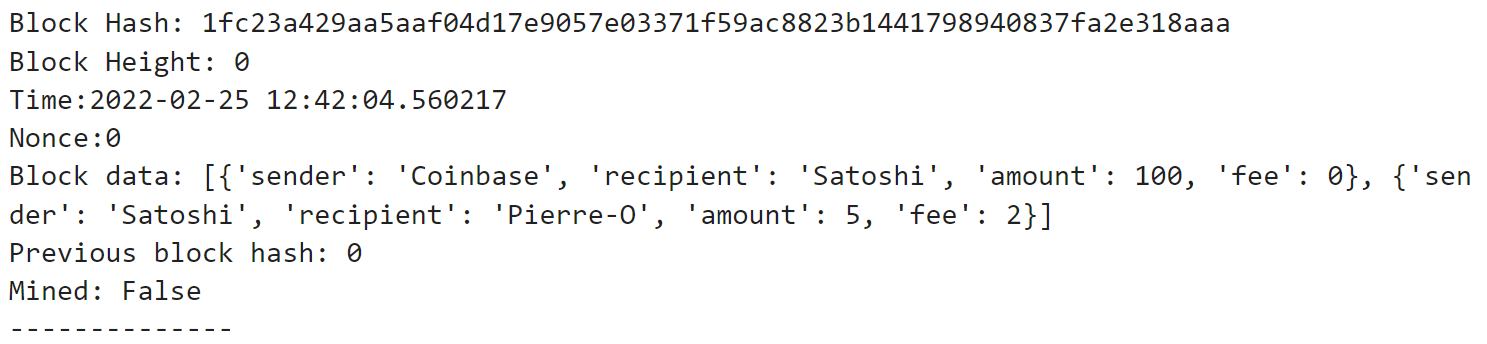
\includegraphics[width = \textwidth]{../Figures/block_not_mined.png}
		\captionsetup{width=0.8\textwidth}
		\centering
		\caption{A block that has not been mined yet.}
		\label{fig:block_not_mined}
\end{figure}
The hash value in decimal notation is $1.43e^{76}$ while the maximum value for a $256$ bits number is $2^{256}-1 \approx 1.16e^{77}$. We refer to the latter as the maximal target and denote it by $T_{\max}$. The Proof-of-Work protocol sets a target $T < T_{\max}$ and ask miners to find a nonce such that the hash value of the block is smaller than $T$. Practitioners would rather talk about the \textit{difficulty} which is defined as $D = T_{\max} / T$. If the difficulty is one, any hash value is acceptable. Increasing the difficulty reduces the set of allowable hash values, making the problem harder to solve. A hash value is then called \textit{acceptable} if its hexadecimal digest starts with a given number of zeros. If we set the difficulty to $2^4$, then the hexadecimal digest of the hash of the block must start with at least $1$ leading zero, making the hash value of the block in Figure \ref{fig:block_not_mined} not acceptable. After completing the nonce search we get the block in Figure \ref{fig:block_mined}.
\begin{figure}[!ht]
		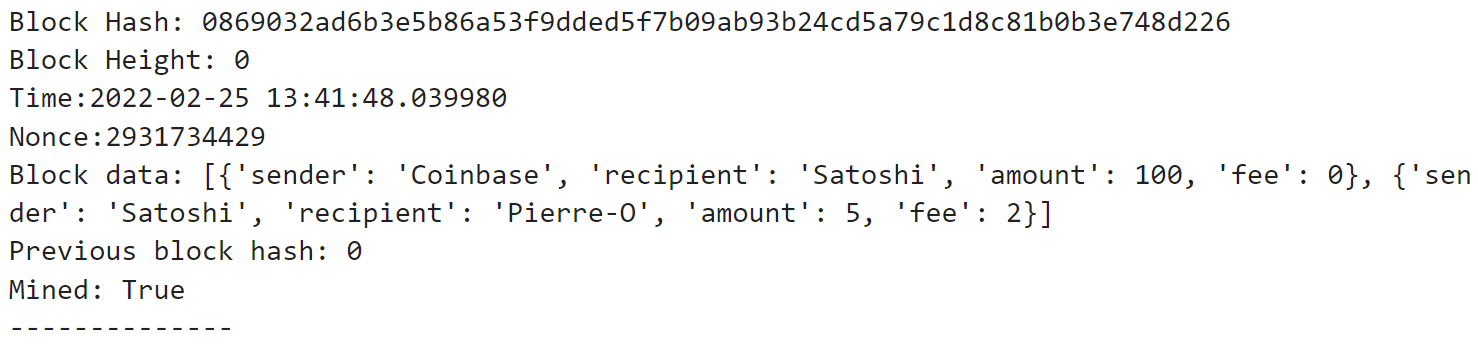
\includegraphics[width = \textwidth]{../Figures/block_mined.png}
		\captionsetup{width=0.8\textwidth}
		\centering
		\caption{A mined block with a hash value having on leading zero.}
		\label{fig:block_mined}
\end{figure}
Note that it took $5$ attempts to find this nonce. The number of needed trials is geometrically distributed with parameter $1 / D$, which means that with a difficulty of $D = 2^4$ it takes on average $16$ trials. The protocol adjusts the difficulty automatically every $2,016$ block discoveries so as to (globally) maintain one block discovery every $10$ minutes on average. The time between two block discoveries depends on the number of hash values computed by the network at a given instant. At the time of writing, the network computes $182.58$ Exahashes per second and the difficulty is $27,967,152,532,434$.\footnote{Source: \href{https://www.bitcoinblockhalf.com/}{bitcoinblockhalf.com}} For an exhaustive overview of the mining process in the bitcoin blockchain, we refer the reader to the book of \citet[Chapter 10]{Antonopoulos2017}. As each trial (of the system) for mining a block is
independent of the others and leads to a success with very small probability, the overall
number of successes is binomially distributed and will be very well approximated by a
Poisson random variable. This justifies the Poisson process assumption made in the sequel to model the block arrival and the reward collecting processes. Empirical studies of the block inter-arrival times data tend to confirm this hypothesis, see the work of Bowden et al.\ \citet{Bowden2020}. The information recorded in a public blockchain may be retrieved by anyone and can be accessed through a blockchain explorer such as \href{https://www.blockchain.com/}{blockchain.com}, the content of the block of height $\#724724$ may be viewed through the following link \href{https://www.blockchain.com/btc/block/0000000000000000000954d42e8ced7017448cb9f39b364e371a1eec6e34463b}{block content}.\\

\noindent The \PoW protocol implies that the nodes are running computations 24/7 therefore consuming humungous quantity of electricity. Bitcoin mining originally started by running computations using the Central Processing Unit (CPU). It turns out that certain kinds of computation are more efficient on Graphics Processing Unit (GPU) than on CPUs. CPU is designed to complete a wide variety of task while computing hashes is very specific. GPU are tailored to run thousands of computation of the same type. Miners then turned to GPUs leading to a shortage of graphics card at the expense of PC gamers around the world! Eventually GPU got replaced by Application Specific Integrated Circuits (ASICs) that are designed to complete very specific task compared to graphic cards. ASICs consumes 10 times more power than graphic cards but compute 10,000 more hashes than a graphic card per time unit. Miners then decided to equip themselves with ASIC chips leading to harmful consequences
\begin{itemize}
    \item Increase of the network electricity consumption
    \item Increase in the e-waste generation. ASICs are single purpose and it cannot be repurpose for any other task. When ASICs become obsolete with the arrival of a new generation of chips, they are thrown in the trash.
    \item The main manufacturer of ASICs is a company called \href{https://www.bitmain.com/}{BITMAIN} which equips major mining pool such as \href{https://v3.antpool.com/home}{Antpool} and \href{https://btc.com}{BTC.com}. A threat on centralization exists since a company like BITMAIN could take control of the network by owning more than half of the overall hashpower.
\end{itemize} 
A pro-ASIC argument is that it would be impossible for anyone (apart from BITMAIN) to suddenly acquire enough of these chips to have more than half of the world's hash power.
\subsection{Proof-of-SpaceTime and Proof-of-Capacity}\label{ssec:posp}
Consensus protocol based on storage capacities are seen by many as a fairer and greener alternative to \PoW. We describe below two such protocols \textit{Proof-of-Capacity} and \textit{Proof-of-Spacetime}.
\subsubsection{Proof-of-Capacity}
In the \textit{Proof-of-Capacity}, miners compute hashes and cache the result on their hard disk space. Mining then only requires to search through the cache for an admissible solution.
\subsubsection{Proof-of-Spacetime}
In the \textit{Proof-of-Spacetime}, the nodes store data and produce proofs to show that the data has been stored for a given time period. The probability of a node being chosen is proportional to the amount of data stored. This protocol has been designed for a specific application allowing nodes to provide storage to clients through the \href{https://filecoin.io/}{Filecoin project}.\\

\noindent To some extent the \textit{Proof-of-Capacity} protocol is similar to \PoW while the \textit{Proof-of-Spacetime} shares similarities with the \textit{Proof-of-Stake} protocol which is discussed below.\\

\noindent Such protocols do not generate ewaste because disk space can always be used for some other purpose. Storing data is less energy consuming than computing hashes. The problem of hiring external storage capacities from provider remains.
\subsection{Proof-of-Interaction}\label{ssec:poi}
The \textit{Proof-of-Interaction} protocol, introduced by \citet{Abegg2021}, asks each validating node to get in touch with a sequence of nodes. The number of nodes and the nodes to be contacted are drawn randomly so that the time to complete the task is also varying from one node to another. The block reward is shared by the contacting and responding nodes to create an incentive compatible environment. If we assume that the time required to complete the task is exponentially distributed then the time to generate a new block is the minimum of exponential random variables which is again exponentially distributed. 
\PoI is still in the developping phase and many interesting work must be done to assess the security and viability of such protocol. Some nodes may indeed collude to send replies faster or not to send replies to some node. It is necessary to evaluate the probability and the opportunity for the nodes to collude.
\subsection{Proof-of-Stake}\label{ssec:pos}
Besides bandwidth, computing power and storage, one ressource that appears with the advent of cryptocurrencies as medium-of-exchange and store-of-value asset are the cryptocoins. Each time a block must be appended to the blockchain, a coin is drawn at random. The owner of that coin appends a new block and collect the reward. \\

\noindent Let the network be of size $N$. We denote by $\pi_i^t$ the proportion of coins owned by node $i\in\{1,\ldots,n\}$ at time $t\in\mathbb{N}$. Note that $\pi_i^t$ is exactly the probability of node $i$ being elected as leader at time $t$, we have
$$
\begin{cases}
\pi_i^t>0,\\
\sum_{i=1}^N\pi_i^t = 1,
\end{cases}
\text{ for } t>0.
$$
Denote by $S_t$ the total number of coins in circulation at time $t$ and by $R_t$ the size of the reward for appending a new block at time $t$. Let $A_i^t$ be the event of node $i$ appending a block at time $t$, the share of coins then evolves as
$$
\pi_i^t = \frac{S\cdot \pi_i^0 + \sum_{s=1}^{t-1}\mathbb{I}_{A_i^t}R_s}{S+\sum_{s=1}^{t-1}R_s},
$$
where 
$$
\mathbb{I}_{A} = \begin{cases}1& \text{if A occurs},\\
0&\text{otherwise}.
\end{cases}
$$
Two potential issues needs to be studied
\begin{itemize}
    \item The Nothing-at-Stake (NaS) problem: If a a fork is ongoing then each branch will elect a leader who will append a block, collect the reward and perpetuate the disabreement.
    \item The rich get richer problem: When a node is chosen, it becomes richer which increase its likelihood to be chosen in future rounds.
\end{itemize}
The "rich get richer" problem will be extensively studied in \cref{chap:decentralization}. Regarding the NaS problem, the nodes when chosen by a branch decide whether they want to add a block, it is an option. The cryptocoin value comes from its use as a medium of exchange. A long lasting disagreement results in a useless cryptocoin with no value.\\

\noindent Let $\tau$ be the duration of the fork and let $\delta\in(0,1)$ be a discount rate, then the present value of a coin at $\tau$ is $1/(1+\delta)^\tau$. If $\mathbb{P}(\tau=\infty)>0$ then the coin value is zero when taking the expectation.\\

\noindent The nodes are therefore incentivized to follow the Longest chain rule in order to resolve the fork situation as soon as possible. This is essentially the rationale in \citet{Saleh2020} to show that 
\begin{itemize}
    \item The coin value reaches a maximum if all the nodes follow the longest chain rule
    \item There exists an equilibrium in which the nodes follow the LCR if 
    $$
    \min \pi_i^0 \cdot S\geq\frac{R_0}{\delta(1-\delta)^2},
    $$
    which corresponds to a minimum stake condition.
    \item If $\sum_t R_t < \infty$ then there exist no equilibrium for which 
    $$
    \mathbb{P}(\tau=\infty)>0.
    $$
    A modest reward schedule precludes the posssibility of an ever lasting fork. 
\end{itemize}
A practical implementation of the \PoS protocol to create a cryptocurrency is \href{https://www.peercoin.net/}{PeerCoin}, see the white paper by \citet{ppcoin}. The notion of coin age is introduced, the stake is actually defined by the number of coins times the number of time period during which the coins was hold. When a peer finds a block, a \textit{coinstake} transaction is made that transfers the node its own coin to reset the coin age to zero.  

% !TEX root = ../main_lecture_notes.tex
\chapter{Security of blockchain systems}\label{chap:security}
The security evaluation of blockchain systems consists in calculating the probability of a successful attack on the blockchain. We will focus, in \cref{sec:double_spending}, on the double spending attack which is concern for \PoW powererd cryptocurrency like teh bitcoin one. Security is also at risk when the node have an incentive to deviate from the prescribed protocol. \cref{sec:blockwithholding} discusses the opportunity for miner of \PoW equipped blockchain to resort to blockwithholding strategy to optimize their revenue. 

\section{Double-spending in PoW}\label{sec:double_spending}
A double spending attack aims at generating a concurrent blockchain to replace the main one. Consider the following scenario
\begin{enumerate}
	\item Marie sends to John BTC$10$
	\item The transaction from Marie to John is recorded in the blockchain
	\item John is advised for $\alpha$ confirmation, that is for $\alpha-1$ block to be appended after the block where the Marie to John transaction is recorded
	\item Once $\alpha$ confirmations have been sent, John ships the good
	\item Meanwhile, Marie has started working on her own blockchain version where the Marie to John transaction is replaced by a Marie to Marie transaction
	\item At the shipment date the main blockchain is ahead by $z$ blocks 
	\item Marie's goal is then to work on her blockchain branch to catch up with the main branch. If she manages to to that then her branch will replace the public branch and she recovers her bitcoin. She can therefore spend these bitcoins again hence the name double spending.
\end{enumerate}
The race between the two competing branches of the blockchain is summarized on \cref{fig:dp_illustration}.
\begin{figure}[ht!]
\begin{center}
\begin{tikzpicture}[-, >=stealth', auto, semithick, node distance=1cm]
% \tikzstyle{block} = [rectangle, draw, fill=blue!20,
%     text width=5em, text centered, rounded corners]
\tikzstyle{block}=[rectangle, fill=black,draw=black,thick,text=black,scale=1.5]
\tikzstyle{block}=[rectangle, fill=white,draw=black,thick,text=black,scale=1.5]
\tikzstyle{confirmed block}=[rectangle, fill=white,draw=blue,thick,text=black,scale=1.5]
\tikzstyle{bad block}=[rectangle, fill=white,draw=red,thick,text=black,scale=1.5]
\node[block]    (1)                     {\tiny $\text{M}\rightarrow \text{J}$};
\node[block]    (2)[right of=1]                     {};
\node[block]    (3)[right of=2]                     {};
\node[block]    (4)[right of=3]                     {};
\node[confirmed block]    (5)[right of=4]                     {};

\node[bad block]    (6)[below of=1]         {\tiny $\text{M}\rightarrow \text{M}$};
\node[block]    (7)[right of=6]         {};
\node[block]    (8)[right of=7]         {};
\path
(1) edge[ left]     node{}     (2)
(2) edge[ left]     node{}     (3)
(3) edge[ left]     node{}     (4)
(4) edge[ left]     node{}     (5)
(6) edge[ left]     node{}     (7)
(7) edge[ left]     node{}     (8);

\end{tikzpicture}
\end{center}
\caption{Double spending race illustrated, here we have $\alpha = 4$ and $z = 2$}
\label{fig:dp_illustration}
\end{figure}
\subsection{Random walk model}\label{ssec:double_spending_rw}
We define a discrete time stochastic process $(R_n)_{n\geq0}$ equal to the difference in length between the public and the private branch of the blockchain. At each time step a block is found, it belongs to the main branch with probability $p$ to the other branch with probability $q=1-p$. The parameter $p$ represents the proportion of hashpower owned by the honest miners, while $q$ is that of the attacker. We have
$$
R_0 = z\text{, and  }R_n = z+Y_1+\ldots+ Y_n.
$$
The $Y_i$'s are \iid random variables such that 
$$
\mathbb{P}(Y=1) = p\in (0,1)\text{, and }\mathbb{P}(Y=-1) = 1-p=q,
$$ 
$(R_n)_{n\geq0}$ is therefore a random walk on $\mathbb{Z}$. We assume that $p>q$ so that the attacker does not hold more than half of the total hashpower. Define the double spending time as 
$$
{\tau_0} = \inf\{n>0\text{ ; }R_n = 0\}.
$$
Our goal is to study the distribution of this stopping time with respect to the filtration 
$$
\mathcal{F}_n = \sigma(Y_1,\ldots, Y_n),\text{ }n\geq1.
$$ 
An illustration of this first-hitting time problem is provided in \cref{fig:double_spending_time}.
\begin{figure}[ht!]
\begin{center}
\begin{tikzpicture}
  %Origin and axis
  \coordinate (O) at (0,0);
  \draw[->] (-1,0) -- (9,0) coordinate[label = {below:$n$}] (xmax);
  \draw[->] (0,-0.5) -- (0,3) coordinate[label = {left:$R_n$}] (ymax);
  %Lower linear boundary

 
  %Stochastic process trajectory
  
  \draw (0,0) node[blue,left] {} node{};
  \draw[very thick,blue,-] (0,1) -- (1,1) node[pos=0.5, above] {} ;
  \draw[very thick,dashed,blue] (1,1) -- (1,1.5) node[pos=0.5, right] {};
  \draw[very thick,blue,-] (1,1.5) -- (2,1.5) node[pos=0.5, above] {};
  \draw[very thick,dashed,blue] (2,1.5) -- (2,2) node[pos=0.5, right] {};
  \draw[very thick,blue,-] (2,2) -- (3,2) node[pos=0.5, above] {};
  \draw[very thick,dashed,blue] (3,2) -- (3,1.5) node[pos=0.5, right] {};
  \draw[very thick,blue,-] (3,1.5) -- (4,1.5)node[pos=0.5, above] {};
  \draw[very thick,dashed,blue] (4,1.5) -- (4,1) node[pos=0.5, right] {};  
  \draw[very thick,blue,-] (4,1) -- (5,1) node[pos=0.5, above] {};
  \draw[very thick,dashed,blue] (5,1) -- (5,0.5) node[pos=0.5, right] {};  
  \draw[very thick,blue,-] (5,0.5) -- (6,0.5) node[pos=0.5, above] {};
  \draw[very thick,dashed,blue,-] (6,0.5) -- (6,1) node[pos=0.5, above] {};
   \draw[very thick,blue,-] (6,1) -- (7,1) node[pos=0.5, above] {};
    \draw[very thick,dashed,blue,-] (7,1) -- (7,0.5) node[pos=0.5, above] {};
     \draw[very thick,blue,-] (7,0.5) -- (8,0.5) node[pos=0.5, above] {};
     \draw[very thick,dashed,blue,-] (8,0.5) -- (8,0) node[pos=0.5, above] {};
  %Jump Times
  \draw (1,0) node[black,below] {$1$} node{ \color{black}$\bullet$};
  \draw (2,0) node[black,below] {$2$} node{ \color{black}$\bullet$};
  \draw (3,0) node[black,below] {$3$} node{ \color{black}$\bullet$};
  \draw (4,0) node[black,below] {$4$} node{ \color{black}$\bullet$};
  \draw (5,0) node[black,below] {$5$} node{ \color{black}$\bullet$};
  \draw (6,0) node[black,below] {$6$} node{ \color{black}$\bullet$};
  \draw (7,0) node[black,below] {$7$} node{ \color{black}$\bullet$};
  \draw (8,0) node[black,below] {$8$} node{ \color{black}$\bullet$};
  %Level of the counting process
   \draw (0,0) node[black,below left] {$0$} node{ \color{black}$\bullet$};
   \draw (0,0.5) node[black,left] {$1$} node{ \color{black}$\bullet$};
   \draw (0,1) node[black,left] {$z=2$} node{ \color{black}$\bullet$};
   \draw (0,1.5) node[black,left] {$3$} node{ \color{black}$\bullet$};
   \draw (0,2) node[black,left] {$4$} node{ \color{black}$\bullet$};
   \draw (0,2.5) node[black,left] {$5$} node{ \color{black}$\bullet$};

  % %Aggregated Capital gains
%  \draw (0,1.5) node[blue,below right] {$\mu_1$} node{ \color{blue}$-$};
%  \draw (0,2.25) node[blue,left] {$\mu_2$} node{ \color{blue}$-$};
%  \draw (0,3.75) node[blue,left] {$\mu_3$} node{ \color{blue}$-$};
  %Ruin time = First-crossing time time
%  \draw (5,0) node[black,above right] {${\tau_0}_u$} node{ \color{black}$\times$};
%  \draw[dotted,black] (0,3.28) -- (5,3.28);
%  \draw[dotted,black] (5,0) -- (5,3.28);
\end{tikzpicture}
\end{center}
\caption{Illustration of the first-hitting time problem of a double spending attack.}
\label{fig:double_spending_time}
\end{figure}
Let us denote by 
$$
\mathbb{P}_z(\cdot) = \mathbb{P}(\cdot|R_0 = z)\text{ and }\mathbb{E}_z(\cdot) = \mathbb{E}(\cdot|R_0 = z) 
$$
We are interested for now in the conditional distribution of ${\tau_0}$ provided that $R_0 = z$.
\subsubsection{Double spending probability}\label{sssec:double_spending_rw_dsp}
The double spending probability is defined as 
$$
\phi(z)=\mathbb{P}_z({\tau_0} <\infty),
$$
and given in the following result
\begin{theo}
If $p>q$ then 
$$
\phi(z) = \left(\frac{q}{p}\right)^z.
$$
\end{theo}
\noindent We give two proofs for this result, the first one uses simple first step analysis exploiting the Markov property of the random walk. The second one uses Martingale and the optional stopping theorem.\\

\underline{\textit Proof 1:}\\
Using a first step analysis, we have 
\begin{equation}\label{eq:difference_equation}
\phi(z) = p\phi(z+1)+(1-p)\phi(z-1),\text{ }z\geq1.
\end{equation}
We also have the boundary conditions
\begin{equation}\label{eq:boundary_conditions_double_spending}
\phi(0) = 1\text{ and }\underset{z\rightarrow +\infty}{\lim}\phi(z) = 0
\end{equation}
Equation \eqref{eq:difference_equation} is a linear difference equation of order $2$ associated to the following characteristic equation
$$
px^2 - x + 1-p = 0
$$
which has two roots on the real line with 
$$
r_1 = 1, \text{ and }r_2 = \frac{1-p}{p}.
$$
The solution of \eqref{eq:difference_equation} is given by 
$$
\phi(z)=A+B\left(\frac{1-p}{p}\right)^z,
$$
where $A$ and $B$ are constant. Using the boudary conditions \eqref{eq:boundary_conditions_double_spending}, we deduce that
$$
\phi(z) = \left(\frac{1-p}{p}\right)^z
$$
as announced.\\
For the second proof we need the notion of martingale
\begin{definition}
A stochastic process $(X_n)_{n\geq0}$, is called a martingale with respect to a filtration $\mathcal{F}_n$, if
\begin{itemize}
  \item[(i)] $X_n$ is $\mathcal{F}_n$-adapted
  \item[(ii)] $\mathbb{E}(X_n)<\infty\text{ for }n\geq\geq0$ 
  \item[(iii)] $\mathbb{E}(X_n|\mathcal{F}_{n-1}) = X_{n-1}$
\end{itemize} 
\end{definition}
\noindent and the optional stopping theorem.
\begin{theo}
Let $T$ be a stopping time for the Martingale $(X_n)_{n\geq0}$ then it holds that 
$$
\mathbb{E}(X_T) = \mathbb{E}(X_0) 
$$
in each of the following situations
\begin{itemize}
\item[(i)] $T$ is bounded almost surely 
\item[(ii)] There exists $c>0$ such that $|X_{T\land n}|<c$ for every $n>0$.
\item[(iii)] $\mathbb{E}(T)<\infty$, and, for some $K>0$ we have that 
$$
|X_n(\omega) - X_{n-1}(\omega)|\leq K,\text{ }\forall (n,\omega).
$$
\end{itemize}

\end{theo}
\underline{\textit Proof 2:}\\
Define the process 
$$
X_n = \exp\left[sR_n- n\kappa_Y(s)\right],\text{ for }n\in\mathbb{N}\text{ and }s\in\mathbb{R}, 
$$
where
$$
\kappa_Y(s) = \log\left[\mathbb{E}\left(e^{sY}\right)\right],
$$
is the cumulant generating function of $Y$. 
\begin{lemma}\label{lem:wald_martingale_RW}
Take $s$ so that $\kappa_Y(s)<\infty$ then $(X_n)_{n\geq0}$ is a $\mathcal{F}_n$-martingale.
\end{lemma}
\begin{proof}
Denote by $M_Y(s) = \mathbb{E}(e^{sY})$ the moment generating function of $Y$, we have that 
\begin{eqnarray*}
\mathbb{E}(X_n|\mathcal{F}_n)&=&\mathbb{E}\left\{\exp\left[sR_n - n\kappa_Y(s)\right]|\mathcal{F}_n\right\}\\
&=&\exp\left[sR_{n-1} - n\kappa_Y(s)\right]\mathbb{E}\left[\exp\left(sY_{n}\right)|\mathcal{F}_n\right]\\
&=&\exp\left[sR_{n-1} \right]M_Y(s)^{-n} M_Y(s)\\
&=& X_{n-1}.
\end{eqnarray*}
\end{proof} 
The equation $\kappa_Y(s) = 0$ is equivalent to 
$$
pe^s+qe^{-s} = 1
$$
which admits $\gamma =\log(q/p)$ as only non-zero solution. The process $(\e^{\gamma R_n})_{n\geq0}$ is a $\mathcal{F}_n$-Martingale. Define $\tau_a = \inf\{n\geq 0\text{ ; }R_n = a\}$, for $a>z$. Consider the stopping time $\tau = \tau_0\land\tau_a$, we have that for any $n>0$, 
$$
\mathbb{P}( \tau=\infty) \leq \mathbb{P}( \tau > n) < \mathbb{P}( |R_n| \leq a) \underset{n\rightarrow \infty}{\longrightarrow} 0;
$$
We can therefore apply the optional stopping time theorem at $\tau$ to get
\begin{eqnarray*}
 \mathbb{E}(X_{\tau}) = \mathbb{E}(X_{0})&\Leftrightarrow& \mathbb{P}(\tau = \tau_0) + [1- \mathbb{P}(\tau = \tau_0)]\e^{a z}= \e^{\gamma z}\\
 &\Leftrightarrow& \mathbb{P}(\tau = \tau_0)] = \frac{\e^{\gamma z}-\e^{a z}}{1-\e^{az}}.
\end{eqnarray*}
We then let $a\rightarrow\infty$ in the above equation to conclude that 
$$
\mathbb{P}(\tau = \tau_0) =\left(\frac{q}{p}\right)^z.
$$
\begin{exercise}
Just for fun
\begin{itemize}
\item What is $\phi(z)$ when $p \leq q$ ? 
\item Compute $\mathbb{P}(\tau_0 \leq \tau_a)$ if $p = q = 1/2$
\end{itemize}
\end{exercise}
In practice the number of blocks $z$ is actually random variable 
$$
Z = (\alpha -M)_+,
$$ 
where $M$ corresponds to the number of blocks the attacker managed to mine while the vendor waits for $\alpha$ confirmations. If we assume that a block mined by the honest miners is a success while a block mined by the attacker is a failure then $M$ actually counts the number of failure before $\alpha$ successes. We have that $M\sim \text{Neg-Bin}(\alpha, p)$ where $M$ has a probability mass function (\pmf) given by 
$$
\mathbb{P}(M = m) = \binom{\alpha+m-1}{m}p^\alpha q^m.
$$
Whenever $Z = 0$ then double spending occur right away as $\phi(0) =1$. To derive the double spending probability, we condition upon the values of $Z$ via the law of total probability 
$$
\mathbb{P}( \text{Double Spending}) = \mathbb{P}(M\geq \alpha)+\sum_{m = 0}^{\alpha-1}\binom{\alpha+m-1}{m}q^\alpha p^m.
$$
The analysis conducted here is similar to that of \citet{rosenfeld2014analysis}.
\subsubsection{Double spending time}\label{sssec:double_spending_rw_dst}
In the block mining world time is money. Every hour spent in computing hashes is costly in terms of energy. It is then very interesting to know whether a double spending attack is meant to last long or not. Intuitively, we can think that if it must occur the it should at a earlier stage because as $p>1/2$ our random walk $(R_n)_{n\geq0}$ will eventually drift toward $+\infty$. The following result provides the probability distribution of $\tau_0$ when $R_0 = z$.
\begin{theo}
If $z = 0$ then $\tau_0=0$ almost surely. If $z>0$ then $\tau_0$ admits a \pmf given by 
$$
\mathbb{P}_z(\tau_0 = n)=
\frac{z}{n}\binom{n}{(n-z) / 2}p^{(n-z) / 2}q^{(n
+z) / 2}\text{ if }n>z\text{ and }n-z\text{ is even},
$$
and $0$ otherwise.
\end{theo}
\begin{proof}
We start by showing the following lemma, sometimes referred to as the Markov hitting time theorem.
\begin{lemma}\label{lem:markov_hitting_time}
\begin{equation}\label{eq:markov_hitting_time}
\mathbb{P}_z(\tau_0 = n) = \frac{z}{n}\mathbb{P}_z(R_n = 0)
\end{equation}
\end{lemma}
\begin{proof}
If $z = 0$ then $\tau_0 = 0$ almost surely and both sides of \eqref{eq:markov_hitting_time} equal to $0$. Assume that $z\geq1$, we have that $\mathbb{P}_z(\tau_0 = n) = 0$ and $\mathbb{P}_z(R_n = 0) = 0$ whenever $n<z$ and $n-z$ is odd. The rest of the proof is by induction on $n\geq1$, when $n = 1$ we have that 
$$
\mathbb{P}_z(\tau_0 = 1) = 0 = \frac{z}{1}\mathbb{P}_z(R_1 = 0),\text{ for }z>1, 
$$
and 
$$\mathbb{P}_1(\tau_0 = 1) = q = \frac{1}{1}\mathbb{P}_1(R_1 = 0),\text{ for }z=1. 
$$
The property holds for $n=1$. Assume that it holds for some $n\geq1$. The law of total probability yields
\begin{eqnarray*}
\mathbb{P}_z(\tau_0 = n+1)&=&\sum_{y\in\{-1,1\}}\mathbb{P}_z(\tau_0 = n+1|Y_1 = y)\mathbb{P}(Y_1 = y)\\
&=&\sum_{y\in\{-1,1\}}\mathbb{P}_{z+y}(\tau_0 = n)\mathbb{P}(Y_1 = y)\\
&=&\sum_{y\in\{-1,1\}}\frac{z+y}{n}\mathbb{P}_{z+y}(R_n = 0)\mathbb{P}(Y_1 = y)
\end{eqnarray*}
The second equality holds thanks to the strong Markov property. We further undo the law of total probability.
\begin{eqnarray}
\mathbb{P}_z(\tau_0 = n+1)&=&\sum_{y\in\{-1,1\}}\frac{z+y}{n}\mathbb{P}_{z}(Y_1 = y|R_{n+1} = 0)\mathbb{P}_z(R_{n+1} = 0)\nonumber\\
&=&\frac{\mathbb{P}_z(R_{n+1} = 0)}{n}\left[z+\mathbb{E}(Y_1|R_{n+1}=0)\right]\label{eq:law_total_probability_undone}
\end{eqnarray}
Since the $Y_i$ are \iid then it holds that 
$$
\mathbb{E}(Y_1|R_{n+1}=0) = \mathbb{E}(Y_i|R_{n+1}=0)\text{, } i = 1, \ldots, n+1,
$$
and it follows that 
$$
\mathbb{E}(Y_1|R_{n+1}=0) = \frac{1}{n+1}\sum_{i =1}^{n+1}\mathbb{E}(Y_i|R_{n+1}=0) = \frac{-z}{n+1}.
$$
Inserting the above expression in \eqref{eq:law_total_probability_undone} yields 
$$
\mathbb{P}_z(\tau_0 = n+1) = \frac{z}{n+1}\mathbb{P}_z(R_{n+1} = 0).
$$
\end{proof}
\begin{remark}
This proof is direct, simple and inspired from \citet{Hofstad2008}. It is possible to make it shorter taking advantage of the ballot theorem. Indeed consider again the first hitting problem on \cref{fig:double_spending_time} and reverse the timeline. It corresponds to that of a random walk $(S_n)_{n\geq0}$ that starts at $0$, make upward jumps with probability $q$, and aims at reaching the level $z$ without crossing the $X$ axis, see \cref{fig:time_reversed_double_spending_time}.
\begin{figure}[ht!]
\begin{center}
 \subfloat[Original first hitting problem]
 {
\begin{tikzpicture}
  %Origin and axis
  \coordinate (O) at (0,0);
  \draw[->] (-1,0) -- (9,0) coordinate[label = {below:$n$}] (xmax);
  \draw[->] (0,-0.5) -- (0,3) coordinate[label = {left:$R_n$}] (ymax);
  %Lower linear boundary

 
  %Stochastic process trajectory
  
  \draw (0,0) node[blue,left] {} node{};
  \draw[very thick,blue,-] (0,1) -- (1,1) node[pos=0.5, above] {} ;
  \draw[very thick,dashed,blue] (1,1) -- (1,1.5) node[pos=0.5, right] {};
  \draw[very thick,blue,-] (1,1.5) -- (2,1.5) node[pos=0.5, above] {};
  \draw[very thick,dashed,blue] (2,1.5) -- (2,2) node[pos=0.5, right] {};
  \draw[very thick,blue,-] (2,2) -- (3,2) node[pos=0.5, above] {};
  \draw[very thick,dashed,blue] (3,2) -- (3,1.5) node[pos=0.5, right] {};
  \draw[very thick,blue,-] (3,1.5) -- (4,1.5)node[pos=0.5, above] {};
  \draw[very thick,dashed,blue] (4,1.5) -- (4,1) node[pos=0.5, right] {};  
  \draw[very thick,blue,-] (4,1) -- (5,1) node[pos=0.5, above] {};
  \draw[very thick,dashed,blue] (5,1) -- (5,0.5) node[pos=0.5, right] {};  
  \draw[very thick,blue,-] (5,0.5) -- (6,0.5) node[pos=0.5, above] {};
  \draw[very thick,dashed,blue,-] (6,0.5) -- (6,1) node[pos=0.5, above] {};
   \draw[very thick,blue,-] (6,1) -- (7,1) node[pos=0.5, above] {};
    \draw[very thick,dashed,blue,-] (7,1) -- (7,0.5) node[pos=0.5, above] {};
     \draw[very thick,blue,-] (7,0.5) -- (8,0.5) node[pos=0.5, above] {};
     \draw[very thick,dashed,blue,-] (8,0.5) -- (8,0) node[pos=0.5, above] {};
  %Jump Times
  \draw (1,0) node[black,below] {$1$} node{ \color{black}$\bullet$};
  \draw (2,0) node[black,below] {$2$} node{ \color{black}$\bullet$};
  \draw (3,0) node[black,below] {$3$} node{ \color{black}$\bullet$};
  \draw (4,0) node[black,below] {$4$} node{ \color{black}$\bullet$};
  \draw (5,0) node[black,below] {$5$} node{ \color{black}$\bullet$};
  \draw (6,0) node[black,below] {$6$} node{ \color{black}$\bullet$};
  \draw (7,0) node[black,below] {$7$} node{ \color{black}$\bullet$};
  \draw (8,0) node[black,below] {$8$} node{ \color{black}$\bullet$};
  %Level of the counting process
   \draw (0,0) node[black,below left] {$0$} node{ \color{black}$\bullet$};
   \draw (0,0.5) node[black,left] {$1$} node{ \color{black}$\bullet$};
   \draw (0,1) node[black,left] {$z=2$} node{ \color{black}$\bullet$};
   \draw (0,1.5) node[black,left] {$3$} node{ \color{black}$\bullet$};
   \draw (0,2) node[black,left] {$4$} node{ \color{black}$\bullet$};
   \draw (0,2.5) node[black,left] {$5$} node{ \color{black}$\bullet$};

  % %Aggregated Capital gains
%  \draw (0,1.5) node[blue,below right] {$\mu_1$} node{ \color{blue}$-$};
%  \draw (0,2.25) node[blue,left] {$\mu_2$} node{ \color{blue}$-$};
%  \draw (0,3.75) node[blue,left] {$\mu_3$} node{ \color{blue}$-$};
  %Ruin time = First-crossing time time
%  \draw (5,0) node[black,above right] {${\tau_0}_u$} node{ \color{black}$\times$};
%  \draw[dotted,black] (0,3.28) -- (5,3.28);
%  \draw[dotted,black] (5,0) -- (5,3.28);
\end{tikzpicture}
\label{subfig:ds_RW_time}
}
\hskip1em
\subfloat[Time reversed first hitting problem]{
\begin{tikzpicture}
  %Origin and axis
  \coordinate (O) at (0,0);
  \draw[->] (-1,0) -- (9,0) coordinate[label = {below:$n$}] (xmax);
  \draw[->] (0,-0.5) -- (0,3) coordinate[label = {left:$S_n$}] (ymax);
  %Lower linear boundary

 
  %Stochastic process trajectory
  
  \draw (0,0) node[blue,left] {} node{};
  \draw[very thick,blue,-] (0,0) -- (1,0) node[pos=0.5, above] {} ;
  \draw[very thick,dashed,blue] (1,0) -- (1,0.5) node[pos=0.5, right] {};
  \draw[very thick,blue,-] (1,0.5) -- (2,0.5) node[pos=0.5, above] {};
  \draw[very thick,dashed,blue] (2,0.5) -- (2,1) node[pos=0.5, right] {};
  \draw[very thick,blue,-] (2,1) -- (3,1) node[pos=0.5, above] {};
  \draw[very thick,dashed,blue] (3,1) -- (3,0.5) node[pos=0.5, right] {};
  \draw[very thick,blue,-] (3,0.5) -- (4,0.5)node[pos=0.5, above] {};
  \draw[very thick,dashed,blue] (4,0.5) -- (4,1) node[pos=0.5, right] {};  
  \draw[very thick,blue,-] (4,1) -- (5,1) node[pos=0.5, above] {};
  \draw[very thick,dashed,blue] (5,1) -- (5,1.5) node[pos=0.5, right] {};  
  \draw[very thick,blue,-] (5,1.5) -- (6,1.5) node[pos=0.5, above] {};
  \draw[very thick,dashed,blue,-] (6,1.5) -- (6,2) node[pos=0.5, above] {};
   \draw[very thick,blue,-] (6,2) -- (7,2) node[pos=0.5, above] {};
    \draw[very thick,dashed,blue,-] (7,2) -- (7,1.5) node[pos=0.5, above] {};
     \draw[very thick,blue,-] (7,1.5) -- (8,1.5) node[pos=0.5, above] {};
     \draw[very thick,dashed,blue,-] (8,1.5) -- (8,1) node[pos=0.5, above] {};
  %Jump Times
  \draw (1,0) node[black,below] {$1$} node{ \color{black}$\bullet$};
  \draw (2,0) node[black,below] {$2$} node{ \color{black}$\bullet$};
  \draw (3,0) node[black,below] {$3$} node{ \color{black}$\bullet$};
  \draw (4,0) node[black,below] {$4$} node{ \color{black}$\bullet$};
  \draw (5,0) node[black,below] {$5$} node{ \color{black}$\bullet$};
  \draw (6,0) node[black,below] {$6$} node{ \color{black}$\bullet$};
  \draw (7,0) node[black,below] {$7$} node{ \color{black}$\bullet$};
  \draw (8,0) node[black,below] {$8$} node{ \color{black}$\bullet$};
  %Level of the counting process
   \draw (0,0) node[black,below left] {$0$} node{ \color{black}$\bullet$};
   \draw (0,0.5) node[black,left] {$1$} node{ \color{black}$\bullet$};
   \draw (0,1) node[black,left] {$z=2$} node{ \color{black}$\bullet$};
   \draw (0,1.5) node[black,left] {$3$} node{ \color{black}$\bullet$};
   \draw (0,2) node[black,left] {$4$} node{ \color{black}$\bullet$};
   \draw (0,2.5) node[black,left] {$5$} node{ \color{black}$\bullet$};

  % %Aggregated Capital gains
%  \draw (0,1.5) node[blue,below right] {$\mu_1$} node{ \color{blue}$-$};
%  \draw (0,2.25) node[blue,left] {$\mu_2$} node{ \color{blue}$-$};
%  \draw (0,3.75) node[blue,left] {$\mu_3$} node{ \color{blue}$-$};
  %Ruin time = First-crossing time time
%  \draw (5,0) node[black,above right] {${\tau_0}_u$} node{ \color{black}$\times$};
%  \draw[dotted,black] (0,3.28) -- (5,3.28);
%  \draw[dotted,black] (5,0) -- (5,3.28);
\end{tikzpicture}
\label{subfig:time_reversed_ds_RW_time}
}
\end{center}
\caption{Another look at the first hitting time problem.}
\label{fig:time_reversed_double_spending_time}
\end{figure}
Note that \cref{subfig:time_reversed_ds_RW_time} is the reflection of \cref{subfig:ds_RW_time} with respect to the $Y$ axis. We have equivalently
$$
\mathbb{P}_z(\tau_0) = \mathbb{P}(S_k>0,\text{ }1\leq k\leq n|S_n = z, S_0 = 0)\mathbb{P}_0(S_n = z|S_0=0),
$$
and 
$$
\mathbb{P}(S_k>0,\text{ }1\leq k\leq n|S_n = z, S_0 = 0) = \frac{z+(n-z)/2-(n-z)/2}{n} = \frac{z}{n}.
$$
For proof of the ballot theorem, see \citet{Renault2007}. For a general formulation and application to queueing see \citet{Takacs1962}.
\end{remark}
To complete the proof, we just note that 
$$
\mathbb{P}_z(R_n = 0) = \binom{n}{(n-z) / 2}p^{(n-z) / 2}q^{(n
+z) / 2}
$$
as it corresponds to a trajectory of $(R_n)_{n \geq0}$ starting at $R_0 = z$ ending at $0$ made of $(n-z)/2$ upward jumps and $(n+z)/2$ downward one.
\end{proof}
Just like in the previous section, the actual double spending time depends on the value of the random variable $Z = (\alpha -M)_+$.

\subsection{Counting process model}\label{sec:counting_process}
Our aim is to go from the discrete time framework of the previous section to a continuous time. To do so, we will model the length of the blockchain as counting processes. We will consider renewal processes and more specifically Poisson processes. We start by giving some reminders on the exponential distribution and counting processes before studying the double spending time distribution.

\subsubsection{Poisson process, Exponential distributions and friends}\label{sssec:exp_distribution}
\begin{definition}\label{def:counting_process}
A counting process $(N_t)_{t\geq0}$ is a continuous time stochastic process that counts the occurence of an event over time such that
\begin{equation*}
N_0=0\text{ and }N_t=\sum_{k=1}^{+\infty}\mathbb{I}_{T_k\leq t}.
\end{equation*}
where $T_1,T_2,T_3,\ldots$ denote the arrival times, with the convention that $T_0=0$. Let $\Delta^T_0,\Delta^T_1,\Delta^T_2,\ldots$ be the sequence of inter-arrival times defined as
$$
\Delta^T_k=T_{k+1}-T_{k}\text{, }k=0,1,2\ldots.
$$
\end{definition}
A trajectory of a counting process is given in 
\begin{figure}[!h]
\begin{center}
\begin{tikzpicture}[scale=1]
  %Origin and axis
  \coordinate (O) at (0,0);
  \draw[->] (-1,0) -- (8,0) coordinate[label = {below:$t$}] (xmax);
  \draw[->] (0,-0.5) -- (0,5.5) coordinate[label = {left:$N_t$}] (ymax);
  %Lower linear boundary


  %Stochastic process trajectory

  \draw (0,0) node[blue,left] {} node{};
  \draw[very thick,blue,-] (0,0) -- (1,0) node[pos=0.5, above] {$\Delta^T_0$} ;
  \draw[very thick,dashed,blue] (1,0) -- (1,1) node[pos=0.5, right] {};
  \draw[very thick,blue,-] (1,1) -- (1.75,1) node[pos=0.5, above] {$\Delta^T_1$};
  \draw[very thick,dashed,blue] (1.75,1) -- (1.75,2) node[pos=0.5, right] {};
  \draw[very thick,blue,-] (1.75,2) -- (2.75,2) node[pos=0.5, above] {$\Delta^T_2$};
  \draw[very thick,dashed,blue] (2.75,2) -- (2.75,3) node[pos=0.5, right] {};
  \draw[very thick,blue,-] (2.75,3) -- (5,3)node[pos=0.5, above] {$\Delta^T_3$};
  \draw[very thick,dashed,blue] (5,3) -- (5,4) node[pos=0.5, right] {};
  \draw[very thick,blue,-] (5,4) -- (6,4) node[pos=0.5, above] {$\Delta^T_4$};
  \draw[very thick,dashed,blue] (6,4) -- (6,5) node[pos=0.5, right] {};
  \draw[very thick,blue,-] (6,5) -- (8,5) node[pos=0.5, above] {$\Delta^T_5$};
  %Jump Times
  \draw (1,0) node[blue,below] {$T_1$} node{ \color{blue}$\bullet$};
  \draw (1.75,0) node[blue,below] {$T_2$} node{ \color{blue}$\bullet$};
  \draw (2.75,0) node[blue,below] {$T_3$} node{ \color{blue}$\bullet$};
  \draw (5,0) node[blue,below] {$T_4$} node{ \color{blue}$\bullet$};
  \draw (6,0) node[blue,below] {$T_5$} node{ \color{blue}$\bullet$};
  %Level of the counting process
   \draw (0,0) node[black,left] {$0$} node{ \color{black}$\bullet$};
   \draw (0,1) node[black,left] {$1$} node{ \color{black}$\bullet$};
   \draw (0,2) node[black,left] {$2$} node{ \color{black}$\bullet$};
   \draw (0,3) node[black,left] {$3$} node{ \color{black}$\bullet$};
   \draw (0,4) node[black,left] {$4$} node{ \color{black}$\bullet$};
   \draw (0,5) node[black,left] {$5$} node{ \color{black}$\bullet$};
\end{tikzpicture}
\end{center}
\caption{Trajectory of the counting process $(N_t)_{t\geq0}$.}
\label{fig:trajectory_counting_process}
\end{figure}
\begin{definition}\label{def_poisson_process}
A Poisson process $(N_t)_{t\geq0}$ is a counting process whose inter-arrival times are \iid exponential random variables.
\end{definition}
\begin{remark}\label{def_renewal_process}
A Poisson process belongs to the family renewal processes which are counting process with \iid inter-arrival times.
\end{remark}
\begin{definition}\label{def:exp_dist}
A random variable $X$ is exponentially distributed $X\sim\ExpDist(\lambda)$ if it has \pdf
$$
f_X(x) =\begin{cases} 
\lambda\e^{-\lambda x},&\text{ if }x>0,\\
0,&\text{ otherwise}.
\end{cases}
$$
\end{definition}
For some reasons, we need to introduce the joint distribution of the order statistics of a uniform random sample.
\begin{prop}\label{def:uniform_OS_dist}
Let $U_1,\ldots, U_n$ be a sample of \iid uniform random variables on $(a,b)$. Denote by 
$$
U_{(1)}\leq U_{(2)}\leq\ldots\leq U_{(n)}
$$
the order statistics of such a sample. The joint distribution of $(U_{(1)},\ldots,  U_{(n)})$ is given by 
$$
f_{(U_{(1)},\ldots, U_{(n)})}(u_1,\ldots, u_n)=\frac{n!}{(b-a)^n}\mathbb{I}_{a<u_1<\ldots< u_n<b}(u_1,\ldots, u_n).
$$
and we denote $(U_{(1)},\ldots,  U_{(n)})\sim \text{OS}_n([a,b])$
\end{prop}
\begin{proof}
Let $g:\mathbb{R}^n\mapsto \mathbb{R}_+$ be measurable and bounded. We have that
$$
\mathbb{E}[g(U_{(1)},\ldots,U_{(n)})]=\mathbb{E}\left[\sum_{\sigma\in\mathcal{S}_n}
g(U_{\sigma(1)},\ldots,U_{\sigma(n)})
\mathbb{I}_{U_{\sigma(1)} <\ldots< U_{\sigma(n)}}
\right]
$$
where $\mathcal{S}_n$ the set of all the permutation of $\{1,\ldots,n \}$. We note that
\begin{eqnarray*}
\mathbb{E}\left[g(U_{\sigma(1)},\ldots,U_{\sigma(n)})
\mathbb{I}_{U_{\sigma(1)} <\ldots< U_{\sigma(n)}}
\right]&=& \mathbb{E}\left[g(U_{1},\ldots,U_{n})
\mathbb{I}_{U_{1} <\ldots< U_{n}}\right]\\
&=&\int_{\mathbb{R}^{n}}g(u_{1},\ldots,u_{n})
\mathbb{I}_{u_{1} <\ldots< u_{n}}\frac{1}{(b-a)^n}\text{d}\lambda_{n}(u_1,\ldots, u_n).
\end{eqnarray*}
It then follows that
$$
\mathbb{E}[g(U_{(1)},\ldots,U_{(n)})]=\int_{\mathbb{R}^{n}}g(u_{1},\ldots,u_{n})
\mathbb{I}_{u_{1} <\ldots< u_{n}}\frac{n!}{(b-a)^n}\text{d}\lambda_{n}(u_1,\ldots, u_n).
$$
\end{proof}
We require some additional result about the gamma distribution.
\begin{prop}\label{prop:erlang_dist}
Let $\Delta^T_1,\ldots, \Delta^T_n$ be \iid exponential $\text{Exp}(\lambda)$ random variables, define the sequence $T_k=\sum_{i=1}^{k}\Delta^T_i, k=1,\ldots, n$.
\begin{enumerate}
\item The $T_{k}$'s are gamma distributed, $T_{k}\sim\GammaDist(k,\lambda)$ with \pdf 
$$
f_{T_k}(t)=\frac{t^{k-1}e^{-\lambda t}\lambda^k}{\Gamma(k)},\text{ }t>0,
$$
where $\Gamma(k) = \int_{0}^{\infty}\e^{- x}x^{k-1}\text{d}x$.
\item The joint distribution of $(T_1,\ldots, T_n)$ has \pmf given by
$$
f_{(T_1,\ldots, T_n)}(t_1,\ldots, t_n)=\lambda^n e^{-\lambda t_n }\mathbb{I}_{0<t_1<\ldots< t_n}(t_1,\ldots, t_n)
$$
\item $[(T_1,\ldots, T_n)|T_{n+1}=t]\sim \text{OS}_{n}([0,t])$
\end{enumerate}
\end{prop}
\begin{proof}
\begin{enumerate}
\item We use induction on $k\geq1$. For $k=1$ we have that $\Delta^T_1= T_1$ so the property holds. Assume that the property hold true for some $k$ and consider $k+1$. We note that $T_{k+1}=T_k+\Delta^T_{k+1}$ then
\begin{eqnarray*}
f_{T_{k+1}}(t)&=&\int_{0}^{t}f_{T_k}(x)f_{\Delta^T_{k+1}}(t-x)\text{d}x\\
&=&\int_{0}^{t}\frac{x^{k-1}e^{-\lambda x}\lambda^k}{(k-1)!}\lambda e^{-\lambda(t-x)}\text{d}x\\
&=&\frac{e^{-\lambda t}\lambda^{k+1}}{(k-1)!}\frac{t^k}{k}=\frac{t^k e^{-\lambda t}\lambda^{k+1}}{k!}.
\end{eqnarray*}
\begin{exercise}
Can you propose another way to show this result? Without using induction.
\end{exercise}
\item Let $g:\mathbb{R}^n\mapsto \mathbb{R}_+$ be measurable and bounded, we have
\begin{eqnarray*}
\mathbb{E}[g(T_{1},\ldots,T_n)]&=& \mathbb{E}[g(\Delta^T_{1},\Delta^T_1+\Delta^T_2\ldots,\Delta^T_1+\ldots+ \Delta^T_n)]\\
&=&\int_{\mathbb{R}^n}g(t_{1},\ldots,t_1+\ldots+ t_n)f_{(\Delta^T_{1},\ldots,\Delta^T_n)}(t_1,\ldots,t_n)\text{d}\lambda_n(t_{1},\ldots,t_n)\\
&=&\int_{\mathbb{R}_+^n}g(t_{1},\ldots,t_1+\ldots+ t_n)\lambda^n\e^{-\lambda(t_1+\ldots+t_n)}\text{d}\lambda_n(t_{1},\ldots,t_n)\\
\end{eqnarray*}
Let us apply the following change of variable 
$$
\Phi:(u_{1},\ldots,u_n)\mapsto(u_1, u_{2}-u_1,\ldots,u_n-u_{n-1}):=(t_1,\ldots, t_n),$$
minding the change in the integration domain as 
$$
\Phi(\mathbb{R}_+\times ]u_1,\infty[\times \ldots\times ]u_{n-1},\infty[) = \mathbb{R}^n_+ 
$$
and the Jacobian $\left|\frac{\text{d}\Phi}{\text{d}u}\right|=1$. It follows that
$$
\mathbb{E}[g(T_{1},\ldots,T_n)]=\int_{\mathbb{R}^n} g(u_1,\ldots, u_n)\lambda^{n}e^{-\lambda u_n}\mathbb{I}_{0<u_1<\ldots<u_n}(u_1,\ldots, u_n)\text{d}\lambda_{n}(u_1,\ldots, u_n).
$$
\item We have that 
\begin{eqnarray*}
f_{T_1,\ldots, T_n|T_{n+1}}(t_1,\ldots,t_n|t)
&=&\frac{f_{T_1,\ldots, T_n,T_{n+1}}(t_1,\ldots,t_n,t)}{f_{T_{n+1}(t)}}\\
&=&\frac{n!}{t^n}\mathbb{I}_{0<t_1<\ldots< t_n<t}(t_1,\ldots, t_n, t).
\end{eqnarray*}
\end{enumerate}
\end{proof}
The fact that the Poisson process is a Levy process will be useful later on, so here it is
\begin{prop}
The following statements are equivalent
\begin{enumerate}
\item $(N_t)_{t\geq 0}$ is a Poisson process
\item The stochastic process $(N_t)_{t\geq 0}$ has
\begin{itemize}
\item[(i)] independent increments, it means that for $0<t_1\leq\ldots\leq t_n$, the random variables
$N_{t_1},N_{t_2}-N_{t_1},\ldots,N_{t_{n}}-N_{t_{n-1}}$
are independent.
\item[(ii)] stationnary increments in the sense that the event frequency distribution over some time period of duration $s>0$ only depends on $s$. Indeed, we have that 
$$
N_{t+s}-N_t\sim\PoissonDist(\lambda s),\text{ for }s,t\geq 0.
$$
\end{itemize}
\end{enumerate}
The stochastic processes with independent and stationnary increments are called Levy processes.
\end{prop}
\begin{proof}
\underline{$1 \Rightarrow 2$}\\
Assume that $(N_t)_{t\geq0}$ is a Poisson process and let $0<t_1<\ldots <t_n$ be some times. Consider the folowing probability 
$$
\mathbb{P}\left(N_{t_1} = j_1, N_{t_2}-N_{t_1} = j_2,\ldots, N_{t_n}-N_{t_{n-1}} = j_n\right)
$$
such that $j_1,\ldots, j_n\in \mathbb{N}$. We can rewrite it as 
$$
\mathbb{P}\left(T_{k_1}\leq t_1<T_{k_1+1}, T_{k_2}\leq t_2<T_{k_2+1},\ldots, T_{k_n} \leq t_n<T_{k_n+1}\right),
$$
where $k_i = j_1 + \ldots +j_i, i = 1,\ldots, n$. Conditionning with respect to  $T_{k_n+1}$ yields
\begin{eqnarray*}
&&\mathbb{P}\left(T_{k_1}\leq t_1<T_{k_1+1}, T_{k_2}\leq t_2<T_{k_2+1},\ldots, T_{k_n}\leq t_n<T_{k_n+1}\right)\\
&=&\int_{t_n}^{+\infty}\mathbb{P}\left(T_{k_1}<t_1<T_{k_1+1}, T_{k_2}<t_2<T_{k_2+1},\ldots, T_{k_n}<t_n|T_{k_n +1}=t\right)f_{T_{k_n+1}}(t)\text{d}\lambda(t)\\
&=& \int_{t_n}^{+\infty}\binom{k_n}{j_1,\ldots, j_n}\left(\frac{t_1}{t}\right)^{j_1}\left(\frac{t_2-t_1}{t}\right)^{j_2}\ldots \left(\frac{t_n-t_{n-1}}{t}\right)^{j_n}\frac{e^{-\lambda t}t^{k_n}\lambda^{k_n + 1}}{k_n!}\text{d}\lambda(t)\\
&=&\frac{e^{-\lambda t_1}\left(t_1\right)^{j_1}}{j_1!}\frac{\left(t_2-t_1\right)^{j_2}e^{-\lambda(t_2 - t_1)}}{j_2!}\ldots \frac{\left(t_n-t_{n-1}\right)^{j_n}e^{-\lambda(t_n - t_{n-1})}}{j_n!}
\end{eqnarray*}
From the second to the third equality we simply ask that amomg $k_n$ uniform random variables $j_1$ fall inside $(0,t_1)$, $j_2$ fall inside $(t_1,t_2)$, etc...


\noindent \underline{$2 \Rightarrow 1$}\\
We aim at showing that $(T_1,\ldots, T_n)$ has \pdf given by
\begin{equation}\label{eq:joint_density_arrival_times}
f_{T_1,\ldots, T_n}(t_1,\ldots, t_n)=\lambda^n e^{-\lambda t_n}\mathbb{I}_{0< t_1<\ldots<t_n}.
\end{equation}
Let $t_1,\ldots, t_n$ and $h$ be nonnegative real numbers such that
$$
t_1<t_1+h<t_2<\ldots<t_n<t_n+h,
$$ 
We have
\begin{eqnarray*}
&&\mathbb{P}(t_1<T_1<t_1+h,\ldots,t_n<T_1<t_n+h)\\
&=&\mathbb{P}(N_{t_1}=0,N_{t_1+h}-N_{t_1}=1,\ldots,N_{t_n}-N_{t_{n-1}+h}=0,N_{t_n+h}-N_{t_n}\geq 1)\\
&=&e^{-\lambda t_1}e^{-\lambda h}\lambda h e^{-\lambda [t_2-(t_1+h)]}e^{-\lambda h}\lambda h\ldots e^{-\lambda [t_n-(t_{n-1}+h)]}[1-e^{-\lambda h}] \\
&=&e^{-\lambda t_n}\lambda^{n-1}h^{n-1}[1-e^{-\lambda h}]\\
\end{eqnarray*}
Divide by $h^{n}$ and let $h$ go to $0$ to get \eqref{eq:joint_density_arrival_times}. After applying a change of variable (reciprocal of that used in the proof of \cref{prop:erlang_dist}) to recover the joint distribution of $(\Delta^{T}_1, \ldots, \Delta^{T}_n)$, we see that the later is actually that of an \iid sample of size $n$ of exponential random variables.
\end{proof}
Last but not the least, we establish the order statistic property of the Poisson process.
\begin{prop}
Provided that $\{N_t=n\}$, the jump times $T_1,\ldots,T_n$ have the same distribution as the order statistic of an \iid sample of $n$ uniform random variable on $(0,t)$, namely it holds that
$$
[T_1,\ldots,T_n|N_t=n]\sim \left(U_{(1)}(0,t),\ldots, U_{(n)}(0,t)\right).
$$
\end{prop}
\begin{proof}
We have
\begin{eqnarray*}
&&\mathbb{E}\left[g(T_1,\ldots, T_n)|N_t = n\right]\\
&=&\frac{\mathbb{E}\left[g(T_1,\ldots, T_n)\mathbb{I}_{N_t = n}\right]}{\mathbb{P}(N_t = n)}\\
&=&\frac{\mathbb{E}\left[g(T_1,\ldots, T_n)\mathbb{I}_{T_n \leq t}\mathbb{I}_{T_{n+1} > t}\right]}{\mathbb{P}(N_t = n)}\\
&=&\frac{n!}{e^{-\lambda t}(\lambda t)^n}\int_{\mathbb{R}^{n+1}}g(t_1,\ldots, t_n)\mathbb{I}_{t_n\leq t<t_{n+1}}(t_n,t_{n+1})f_{T_1,\ldots, T_{n+1}}(t_1,\ldots, t_{n+1})\text{d}\lambda_{n+1}(t_1,\ldots, t_{n+1})\\
&=&\frac{n!}{e^{-\lambda t}(\lambda t)^n}\int_{\mathbb{R}^{n}}\int_{t}^{+\infty}g(t_1,\ldots, t_n)\mathbb{I}_{0<t_1<\ldots t_n\leq t}(t_1,\ldots,t_{n})\lambda^{n+1} e^{-\lambda t_{n+1}}\text{d}\lambda_{n+1}(t_1,\ldots, t_{n+1})\\
&=&\frac{n!}{e^{-\lambda t}(\lambda t)^n}\int_{\mathbb{R}^{n}}g(t_1,\ldots, t_n)\mathbb{I}_{0<t_1<\ldots t_n\leq t}(t_1,\ldots,t_{n})\lambda^{n} \text{d}\lambda_{n}(t_1,\ldots,t_n)\e^{-\lambda t}\\
&=&\int_{\mathbb{R}^{n}}g(t_1,\ldots, t_n)\frac{n!}{t^n}\mathbb{I}_{0<t_1<\ldots t_n\leq t}(t_1,\ldots,t_{n})\text{d}\lambda(t_1,\ldots,t_{n} ).
\end{eqnarray*}
\end{proof}
\noindent The order statistic property of the Poisson process will be useful to solve the first hitting time problem arising later on. To fully benefit from this nice property, we need to introduce Appell and Abel-Gontcharov polynomials.\\

\noindent Let $U=\{u_i, \, i\geq 1\}$ be a non-decreasing sequence of real numbers. To $U$ is attached a (unique) family of Appell polynomials of degree $n$ in $x$, $\{A_{n}(x\vert U),\, n\geq 0\}$ defined as follows.
\begin{definition} 
Starting with $A_0(x\vert U)=1$, the $A_n(x\vert U)$'s satisfy the differential equations
\begin{equation}\label{eq:DifferentialEquationAppellPolynomial}
A_{n}^{(1)}(x|U)=nA_{n-1}(x|U),  
\end{equation}
with the border conditions
\begin{equation}\label{eq:Border AppellPolynomial}
A_{n}(u_{n}|U)=0, \quad n\geq 1.
\end{equation}
So, each $A_n$ has the integral representation
\begin{equation}\label{eq:IntegralRepresentationAppellPolynomials}
A_{n}(x|U)=n!\int_{u_{n}}^{x}\left[\int_{u_{n-1}}^{y_{n}}\text{d}y_{n-1} \ldots \int_{u_{1}}^{y_{1}}\text{d}y_{1}\right]\text{d}y_{n}, \quad n\geq 1.
\end{equation}
\end{definition}

In parallel, to $U$ is attached a (unique) family of Abel-Gontcharov (A-G) polynomials of degree $n$ in $x$, $\{G_{n}(x\vert U),\, n\geq 0\}$.
\begin{definition} 
Starting with $G_0(x\vert U)=1$, the $G_n(x\vert U)$'s satisfy the differential equations
\begin{equation}\label{eq:DifferentialEquationAGPolynomials}
G_n^{(1)}(x|U)=nG_{n-1}(x|{\cal E}U), 
\end{equation}
where ${\cal E}U$ is the shifted family $\{u_{i+1}, \, i\geq 1\}$, and with the border conditions
\begin{equation}\label{eq:Border AGPolynomial}
G_{n}(u_{1}|U)=0, \quad  n\geq 1.
\end{equation}
So, each $G_n$ has the integral representation
\begin{equation}\label{eq:IntegralRepresentationAGPolynomials}
G_{n}(x|U)=n!\int_{u_{1}}^{x}\left[\int_{u_{2}}^{y_{1}}\text{d}y_{2} \ldots \int_{u_{n}}^{y_{n-1}}\text{d}y_{n}\right]\text{d}y_{1}, \quad n\geq 1.
\end{equation}
\end{definition}
\noindent The Appell and A-G polynomials are closely related through the identity
\begin{equation}\label{eq:link_AG_Appell}
G_{n}(x|u_{1},\ldots,u_{n})=A_{n}(x|u_{n},\ldots,u_{1}), \quad n\geq 1.
\end{equation}
The two families (i.e. for all $n\geq 0$), however, are distinct and enjoy different properties. From \eqref{eq:IntegralRepresentationAppellPolynomials} and \eqref{eq:IntegralRepresentationAGPolynomials}, it is clear that the polynomials $A_n$ and $G_n$ can be interpreted in terms of the joint distribution of the vector $(U_{1:n},\ldots,U_{n:n})$. 
\begin{prop}
For $0\leq u_1 \leq \ldots \leq u_{n} \leq x \leq 1$,
\begin{equation}\label{eq:ProbabilisticInterpretationAppellPolynomials}
P[U_{(1)} > u_1, \ldots, U_{(n)} > u_{n}\, \mbox{ and }\, U_{(n)}\leq x]= 
A_n(x \vert u_1, \ldots, u_{n}), \quad n\geq1.
\end{equation}
For $0\leq x \leq u_1 \leq \ldots \leq u_{n} \leq 1$,
\begin{equation}\label{eq:ProbabilisticInterpretationAGPolynomials}
P[U_{(1)} \leq u_1, \ldots, U_{(n)} \leq u_{n}\, \mbox{ and }\, U_{(1)}> x]
= (-1)^n \, G_n(x \vert u_1, \ldots, u_{n}), \quad n\geq 1.
\end{equation}
\end{prop}
The representations \eqref{eq:ProbabilisticInterpretationAppellPolynomials} and \eqref{eq:ProbabilisticInterpretationAGPolynomials} will play a key role for solving first-hitting problem that involve Poisson processes. Numerically, it will be necessary to evaluate some special values of the polynomials. To this end, it is convenient to use the following recusive relations. 
\begin{prop} 
The Appell polynomials are computed through the expansion
\begin{equation}\label{eq:appell_polynomials_recursion_1}
A_{n}(x|U)=\sum_{k=0}^{n}\binom{n}{k}A_{n-k}(0|U)x^{k}, \quad n\geq 1,
\end{equation}
where the $A_{n}(0|U)$'s are obtained recursively from 
\begin{equation}\label{eq:appell_polynomials_recursion_2}
A_{n}(0|U)=-\sum_{k=1}^{n} \binom{n}{k} A_{n-k}(0|U)u_{n}^{k}, \quad n\geq1.
\end{equation}
The A-G polynomials are computed through the recursion
\begin{equation}\label{eq:recursion_AG_polynomials}
G_{n}(x|U)=x^{n}-\sum_{k=0}^{n-1} \binom{n}{k} u_{k+1}^{n-k} G_{k}(x|U), \quad n\geq 1.
\end{equation}
\end{prop}
\begin{proof}
The Maclaurin expansion of $A_n(x|U)$ gives \eqref{eq:appell_polynomials_recursion_1} as
$$
A_n(x|U) = \sum_{k = 0}^n\frac{A_n^{(k)}(0|U)}{k!}x^k = \sum_{k = 0}^n\binom{n}{k}A_{n-k}(0|U)x^k.
$$
Evaluation at $x = u_n$ then provides \eqref{eq:appell_polynomials_recursion_2}. Regarding \eqref{eq:recursion_AG_polynomials}, first note that 
$$
G_n^{(k)}(u_{k+1}|U) = \begin{cases}
1,&\text{ if }k = n,\\
0,&\text{ otherwise.}
\end{cases}
$$
Any polynomials $R(x)$ of degree $n$ can therefore be written as 
$$
R(x)=\sum_{k = 0}^n\frac{R^{(k)}(u_{k+1})}{k!}G_k(x|U).
$$
By expanding $x^n$ one gets \eqref{eq:recursion_AG_polynomials}.
\end{proof}
Hereafter are a couple of useful properties
\begin{prop}\label{prop:Appell_AG_polynomials_properties}
\begin{enumerate}
\item For any $a,b\in \mathbb{R}$, it holds that
\begin{equation}
A_{n}(x|a+bU) = b^n A_n\left((x-a)/b \, |U\right), \quad n\geq 1, \label{eq:LinearTransform}
\end{equation}
with the same identity for $G_n$.
\item We have 
\begin{eqnarray}
&&A_{n}(x|1,\ldots,n) = x^{n-1}(x-n), \label{eq:ExplicitExpressionIntAppellPolynomials}\\
&&G_{n}(x|0,\ldots,n-1)= x(x-n)^{n-1}.    \label{eq:ExplicitExpressionIntAGPolynomials}
\end{eqnarray}
\item Let $\{X_{n}\text{ , }n\geq1\}$ be a sequence of \iid nonnegative random variables, of partial sums $S_{n}=\sum_{k=1}^{n}X_{k}$ with $S_0=0$. Then, for $n\geq 1$,
\begin{eqnarray}
&&\mathbb{E} \left[A_{n}(x|S_{1},\ldots,S_{n})\vert S_{n}\right] = x^{n-1}(x-S_{n}), \label{eq:ExplicitExpressionPartialSumsAppellPolynomials}\\
&&\mathbb{E}\left[G_{n}(x|S_{0},\ldots,S_{n-1})\vert S_{n}\right] = x(x-S_{n})^{n-1}.    \label{eq:ExplicitExpressionPartialSumsAGPolynomials}
\end{eqnarray}
\end{enumerate} 
\end{prop}
\begin{proof}
\begin{enumerate}
  \item Let us use induction on $n\geq1$. Take $n = 1$, we have
  $$
  A_1(x|a + bu_1) = \int_{a+bu_1}^{x} A_1'(y|a+bu_1)\text{d}y = x - a - bu_1 
  $$
  and 
   $$
  A_1(x|u_1) = x-u_1.
  $$
  The property holds for $n = 1$. Assume that it holds true for some $n$ and consider $n+1$. We have
  \begin{eqnarray*}
  A_{n+1}(x|a+bU) &=& \int^{x}_{a+b u_{n+1}}A_{n+1}'(y|a+bU)\text{d}y\\
  &=& \int^{x}_{a+b u_{n+1}}nA_{n}(y|a+bU)\text{d}y\\
  &=&b^n\int^{x}_{a+b u_{n+1}}nA_{n}\left(\frac{y-a}{b}\Big|U\right)\text{d}y\\
  &=&b^{n+1}n\int^{\frac{x-a}{b}}_{u_{n+1}}A_{n}\left(z\Big|U\right)\text{d}y\\
  &=&b^{n+1}\int^{\frac{x-a}{b}}_{u_{n+1}}A_{n+1}'\left(z\Big|U\right)\text{d}y\\
  &=&b^{n+1}A_{n+1}\left(\frac{x-a}{b}\Big|U\right),
  \end{eqnarray*}
  so the property holds for $n+1$. No need to do the job for the $G_n(.|U)$'s thanks to \eqref{eq:link_AG_Appell}.
\item Again induction on $n\geq1$. Take $n = 1$, we have
$$
A_1(x|1) = x-1
$$
Assume that the result holds true for some $n$ and consider $n+1$. We have 
\begin{eqnarray*}
A_{n+1}(x|1,\ldots, n,n+1) &=& \int_{n+1}^{x}A_{n+1}'(y|1,2,\ldots, n+1)\text{d}y\\
&=& (n+1)\int_{n+1}^{x}A_{n}(y|1,2,\ldots, n)\text{d}y\\
&=& (n+1)\int_{n+1}^{x}y^{n-1}(y-n)\text{d}y\\
&=& x^n[x - (n + 1)]
\end{eqnarray*}
For identity \eqref{eq:ExplicitExpressionIntAGPolynomials}, write 
\begin{eqnarray*}
G_{n}(x|0,\ldots, n-1)&=&G_{n}(x-n|-n ,\ldots,-1)\\
&=&(-1)^nG_{n}(n-x|n,\ldots, 1)\\
&=&(-1)^nA_{n}(n-x|1,\ldots, n)\\
&=&(-1)^n(n-x)^{n-1}(-x)\\
&=&x(x-n)^{n-1}.
\end{eqnarray*}
\item Again induction on $n\geq1$. Take $n = 1$, we have
$$
\mathbb{E}[A_1(x|S_1)|S_1] = x-S_1
$$
Assume that the result holds true for some $n$ and consider $n+1$. We have 
\begin{eqnarray*}
\mathbb{E}\left[A_{n+1}(x|S_1,\ldots, S_n,S_{n+1})|S_{n+1}\right]&=&\mathbb{E}\left[\int_{S_{n+1}}^x A_{n+1}'(y|S_1,\ldots, S_n,S_{n+1})\text{d}y|S_{n+1}\right]\\
&=&\int_{S_{n+1}}^x\mathbb{E}\left[ A_{n+1}'(y|S_1,\ldots, S_n,S_{n+1})|S_{n+1}\right]\text{d}y\\
&=&(n+1)\int_{S_{n+1}}^x\mathbb{E}\left[A_{n}(y|S_1,\ldots, S_n)|S_{n+1}\right]\text{d}y\\
&=&(n+1)\int_{S_{n+1}}^x\mathbb{E}\left\{\mathbb{E}\left[A_{n}(y|S_1,\ldots, S_n)|S_n,S_{n+1}\right]|S_{n+1}\right\}\text{d}y\\
&=&(n+1)\int_{S_{n+1}}^x\mathbb{E}\left\{\mathbb{E}\left[A_{n}(y|S_1,\ldots, S_n)|S_n\right]|S_{n+1}\right\}\text{d}y\\
&=&(n+1)\int_{S_{n+1}}^x\mathbb{E}\left[y^{n-1}(y-S_n)|S_{n+1}\right]\text{d}y\\
&=&(n+1)\int_{S_{n+1}}^xy^n-\frac{n}{n+1}S_{n+1}y^{n-1} \text{d}y\\
&=&x^n(x-S_{n+1})\\
\end{eqnarray*}
For identity \eqref{eq:ExplicitExpressionPartialSumsAGPolynomials}, write 
\begin{eqnarray*}
\mathbb{E}\left[G_{n}(x|S_0,\ldots, S_{n-1})|S_{n}\right]&=&\mathbb{E}\left[G_{n}(x-S_n|S_0 - S_n,\ldots, S_{n-1}-S_n)|S_{n}\right]\\
&=&(-1)^n\mathbb{E}\left[G_{n}(S_n-x|S_n,\ldots, S_{n}-S_{n-1})|S_{n}\right]\\
&=&(-1)^n\mathbb{E}\left[A_{n}(S_n-x|S_{n}-S_{n-1},\ldots, S_n)|S_{n}\right]\\
&=&(-1)^n(S_n-x -S_n)(S_n-x)^{n-1}\\
&=&x(x-S_n)^{n-1}.\\
\end{eqnarray*}
\end{enumerate}
\end{proof}

\subsubsection{A tiny bit of insurance risk theory}\label{sssec:insurance_risk_theory}
In what follows we will use classical result from insurance risk theory and so we have to provide some context. The financial reserve of a nonlife insurance company can be modelled by a continuous time stochastic process $(R_t)_{t\geq0}$ defined as 
\begin{equation}\label{eq:risk_process}
R_t = u + P_t - L_t,\text{ }t\geq0
\end{equation}
where 
\begin{itemize}
  \item $R_0 = u>0$ are the initial reserves,
  \item $(P_t)_{t\geq0}$ is the premium income process,
  \item $(L_t)_{t\geq0}$ is the liability of the insurance company, that is the sum of all the compensations paid to to the policyholders.
\end{itemize}
The classical assumes that the premium are collected linearly in times at some rate $c$ per time unit. Namely, we have 
$$
P_t = c\times t.
$$
The number of claims is governed by a counting process $(N_t)_{t\geq0}$, usually a standard Poisson process with intensity $\lambda$. To each claim is associated a randomly sized compensation distributed as $U$. The claim sizes $U_1,U_2,\ldots$ form a sequence of \iid random variables independent from $N_t$. We therefore have 
$$
L_t = \sum_{k = 1}^{N_t}U_k.
$$
The name of the game is to compute the ruin probabilities 
\begin{equation}\label{eq:ruin_probabilities}
\psi(u,T) = \mathbb{P}(\tau_0 \leq T),\text{ and }\psi(u) = \mathbb{P}(\tau_0 < \infty),
\end{equation} 
where $\tau_u = \inf\{t\geq0\text{ ; }R_t \leq 0\}$ is the ruin time. This first hitting time problem is illustrated on \cref{fig:ruin_time_CL}
\begin{figure} 
\begin{center}
\begin{tikzpicture}
  %Origin and axis
  \coordinate (O) at (0,0);
  \draw[->] (-0.5,0) -- (5.5,0) coordinate[label = {below:$t$}] (xmax);
  \draw[->] (0,-0.5) -- (0,4) coordinate[label = {right:$R_t$}] (ymax);
   %Initial reserves
  \draw (0,2) node[black,left] {$z$} node{};
 % % %Length of the honest chain
  \draw[thick, blue,-] (0,2) -- (2,3) node[pos=0.5, above] {};
  \draw[thick, dashed, blue] (2,3) -- (2,1) node[pos=0.5, left] {\color{black}$U_1$};
  \draw[thick, blue] (2,1) -- (3,1.5) node[pos=0.5, above] {};
  \draw[thick, dashed, blue] (3,1.5) -- (3, 0.5) node[pos=0.5, left] {\color{black}$U_2$};
  \draw[thick, blue] (3,0.5) -- (5, 1.5) node[pos=0.5, above] {};
   \draw[thick, dashed, blue] (5,1.5) -- (5, -0.5) node[pos=0.5,above left] {\color{black}$U_3$};

  %Block finding Times 
  \draw (2,0) node[black,below] {$T_1$} node{ \color{black}$\bullet$};
  \draw (3,0) node[black,below] {$T_2$} node{ \color{black}$\bullet$};
  \draw (5,0) node[black,below left] {$\tau_u$} node{ \color{black}$\bullet$};
\end{tikzpicture}
\end{center}
\label{fig:ruin_time_CL}
\caption{Illustration of the classical insurance ruin problem}
\end{figure}
This enables to select an initial reserves level $u$ so that the ruin probability is low enough. The premium rate is usually set to compensate the losses due to claims with 
$$
\mathbb{E}(P_t) = (1+\eta)\mathbb{E}(L_t)\text{ or  equivalently } c = (1+\eta)\lambda\mathbb{E}(U).
$$
Define the claim surplus process as
$$
S_t = u - R_t = L_t-P_t,\text{ }t\geq 0.
$$
The following result is the counterpart of \cref{lem:wald_martingale_RW} for Lévy processes.
\begin{prop}\label{prop:wald_martingale_levy}
If $(S_t)_{t\geq0}$ is a L\'evy process then
$$
M_t = \exp\left[\theta S_t-t\kappa(\theta)\right]\text{, }t\geq0,\text{ and }\theta\in \mathbb{R}, 
$$
where $\kappa(\theta)=\log\mathbb{E}\left(e^{\theta S_1}\right)<\infty$, is a martingale.
\begin{proof}
We have that 
\begin{eqnarray*}
\mathbb{E}(M_t|\mathcal{F}_s) &=&\mathbb{E}\left\{\exp\left[\theta S_t-t\kappa(\theta)\right]|\mathcal{F}_s\right\} \\
&=&\e^{-t\kappa(\theta)}\mathbb{E}\left\{\exp\left[\theta (S_t-S_s) + \theta S_s\right]|\mathcal{F}_s\right\}\\
&=&\e^{-t\kappa(\theta)}\e^{\theta S_s}\mathbb{E}\left(\e^{\theta (S_t-S_s)}\right)\\
&=&\e^{-t\kappa(\theta)}\e^{\theta S_s}\e^{(t-s)\kappa(\theta)}\\
&=&\e^{\theta S_s -s\kappa(\theta)}.
\end{eqnarray*}
\end{proof}
\end{prop}
The infinite time horizon ruin probability may be evaluated using the following result.
\begin{prop}\label{prop:ruin_proba_levy}
If $S_t\overset{\textbf{a.s.}}{\rightarrow} -\infty$, and there exists $\gamma>0$ such that $\left(e^{\gamma S_t}\right)_{t\geq0}$ is a martingale then
$$
\mathbb{P}(\tau_u<\infty)=\frac{e^{-\gamma u}}{\mathbb{E}\left[e^{\gamma \xi(u)}|\tau_u<\infty\right]},
$$
where $\xi(u)=S_{\tau_u}-u$ denotes the deficit at ruin.
\end{prop}
\begin{proof}
We apply the optionnal stopping theorem on $(e^{\gamma S_t})_{t\geq0}$ at time $T\land \tau_u$ for some $T>0$ to get 
\begin{eqnarray*}
1 = \mathbb{E}\left(\e^{\gamma S_0}\right)&=& \mathbb{E}\left(\e^{\gamma S_{T\land \tau_u}}\right)\\  
&=& \mathbb{E}\left(\e^{\gamma S_{\tau_u}}\mathbb{I}_{\tau_u\leq T} + \e^{\gamma S_{T}}\mathbb{I}_{\tau_u> T}\right).\\
\end{eqnarray*} 
Letting $T\rightarrow\infty$ yields\footnote{Thanks to $S_t\rightarrow -\infty$, monotone and dominated convergence.}
\begin{eqnarray*}
1 &=&\mathbb{E}\left(\e^{\gamma S_{\tau_u}}\mathbb{I}_{\tau_u<\infty}\right)\\
&=&\e^{\gamma u}\mathbb{E}\left(\e^{\gamma \xi(u))}|\tau_0<\infty\right)\psi(u).
\end{eqnarray*} 
\end{proof}
We will use \cref{prop:ruin_proba_levy} to derive the double spending probability within a continuous time framework in the next sections.
\subsubsection{Double spending probability}\label{sssec:double_spending_counting_process_dsp}
The \textit{Proof-of-Work} protocol implies a steady block arrival, every $10$ minnutes for the bitcoin blockchain. Each trial (of the network) for mining a block is independent of the others and leads to a success with very small probability, the overall number of successes is binomially distributed, very well approximated by a
Poisson random variable. This justifies the Poisson process assumption made in the sequel to model the block arrival.\\

\noindent Denote by $(z+ N_t)_{t\geq 0}$ and $(M_t)_{t\geq 0}$ the number of blocks found by the honest miners and the attackers respectively. Double spending occurs at time 
$$
\tau_z = \inf\{t\geq0\text{ ; }z+N_t = M_t\}.
$$
Assume that $(N_t)_{t\geq 0}$ and $(M_t)_{t\geq 0}$ are Poisson processes with intensity $\lambda$ and $\mu$ such that $\lambda>\mu$. Let $(T_i)_{i\geq0}$ and $(S_i)_{i\geq0}$ be the arrival times of $(N_t)_{t\geq 0}$ and $(M_t)_{t\geq 0}$
The first-hitting problem along with its notation is illustrated in \cref{fig:ds_poisson_process_illustrated}.
\begin{figure}[!ht]
\begin{center}
\begin{tikzpicture}
  %Origin and axis
  \coordinate (O) at (0,0);
  \draw[->] (-0.5,0) -- (5.5,0) coordinate[label = {above:$t$}] (xmax);
  \draw[->] (0,-0.5) -- (0,5) coordinate[label = {right:$n$}] (ymax);
 %Length of the honest chain
  \draw[thick,blue,-] (0,3) -- (2,3) node[pos=0.5, above] {} ;
  \draw[thick,blue] (2,3) -- (2,4) node[pos=0.5, above] {};
  \draw[thick,blue] (2,4) -- (5.5,4) node[pos=0.5, right] {};
  % %Length of the Malicious chain
  \draw[very thick,dashed,red,-] (0,0) -- (0.75,0) node[pos=0.5, above] {} ;
  \draw[very thick,dashed,red] (0.75,0) -- (0.75,1) node[pos=0.5, right] {};
  \draw[very thick,dashed,red] (0.75,1) -- (1.25,1) node[pos=0.5, above] {};
  \draw[very thick,dashed,red] (1.25,1) -- (1.25,2) node[pos=0.5, right] {};
  \draw[very thick,dashed,red] (1.25,2) -- (2.5,2) node[pos=0.5, above] {};
  \draw[very thick,dashed,red] (2.5,2) -- (2.5,3) node[pos=0.5, right] {};
  \draw[very thick,dashed,red] (2.5,3) -- (5,3) node[pos=0.5, right] {};
  \draw[very thick,dashed,red] (5,3) -- (5,4) node[pos=0.5, above] {};
  \draw[very thick,dashed,red] (5,4) -- (5.5,4) node[pos=0.5, above] {};
  %Jump Times of the malicious chain
  \draw (0.75,0) node[red,below] {$S_1$} node{ \color{red}$\bullet$};
  \draw (1.25,0) node[red,below] {$S_2$} node{ \color{red}$\bullet$};
  \draw (2.5,0) node[red,below] {$S_3$} node{ \color{red}$\bullet$};
  \draw (5,0) node[black,below] {$S_4=\tau_z$} node{ \color{black}$\bullet$};
  % %Jump Times of the honest chain
  \draw (2,0) node[blue,below] {$T_1$} node{ \color{blue}$\bullet$};
  % %Aggregated Capital gains
  \draw (0,1) node[black,left] {$1$} node{ \color{black}$-$};
  \draw (0,2) node[black,left] {$2$} node{ \color{black}$-$};
  \draw (0,3) node[black,left] {$z$} node{};
  \draw (0,4) node[black,left] {$4$} node{ \color{black}$-$};
  % %Ruin time = First-meeting time
  % \draw (7,0) node[black,below] {$\tau_z$} node{ \color{black}$\times$};
  % \draw[dotted,black] (7,3) -- (7,0);
\end{tikzpicture}
\end{center}
\caption{Illustration of the double spending problem within a continuous time framework.}
\label{fig:ds_poisson_process_illustrated}
\end{figure}
The double spending probability is given by the following result
\begin{theo}\label{theo:ds_probability_Poisson_process}
The double spending probability is given by 
$$
\mathbb{P}(\tau_z < \infty) = \left(\frac{\mu}{\lambda}\right)^z.
$$
\end{theo}
\begin{proof}
We make an analogy with \cref{sssec:insurance_risk_theory}, where $z$ is the inital reserves, $N_t$ is the premium income and $M_t$ is the liability of an insurance company. Define the claim surplus process as 
$$
S_t = M_t - N_t,\text{ }t\geq0.
$$
Note that $(S_t)_{t\geq0}$ is a L\'evy process such that $S_t\rightarrow + \infty$ beacuse $\lambda >\mu$. The equation 
$$
\kappa(s) =\log\mathbb{E}\left(e^{s S_1}\right) = 0
$$
is equivalent to 
$$
\mu \e^s + \lambda \e^{-s}- (\mu+\lambda) =0,
$$
which has a unique non negative solution given by 
$$
\gamma = \log\left(\frac{\lambda}{\mu}\right).
$$
It follows from \cref{prop:wald_martingale_levy} that $(\e^{\gamma S_t})_{t\geq 0}$ is a martingale, and applying \cref{prop:ruin_proba_levy} yields the double spending probability 
$$
\mathbb{P}(\tau_z<\infty) = \left(\frac{\mu}{\lambda}\right)^z,
$$
since $\xi(z)=0$ as ruin occurs exactly.
\end{proof}
\subsubsection{Double spending time}\label{sssec:double_spending_counting_process_dst}
Just like in \cref{sssec:double_spending_rw_dst}, we are interested in the time required to complete a double spending attack. Accounting for the cost of electricity, we can approximate the operational cost per time unit by 
$$
c = \pi_W\cdot W\cdot q,
$$
where 
\begin{itemize}
  \item $\pi_W$ is the electricity cost
  \item $W$ is the electricity consumed by the network
  \item  $q$ is the attacker's hashpower
\end{itemize}
The double spending cost reduces to $\tau_z\cdot c$. the following result provides a formula for the \pdf of $\tau_z$.
\begin{theo}
If $(N_t)_{t\geq0}$ is a Poisson process and $(M_t)_{t\geq0}$ is a renewal process then the \textbf{p.d.f.} of $\tau_z$ is given by
\begin{equation}\label{eq:DS_time_pdf}
f_{\tau_z}(t)=\mathbb{E}\left[\frac{z}{z+N_t}f_{S_{N_t+z}}(t)\right],\text{ for }t\geq0.
\end{equation}
\end{theo}
\begin{proof}
The event $\{\tau_z\in(t,t+\text{d}t)\}$, for $t\geq0$, corresponds to the exact time at which the double-spending attack is successful as the malicious chain takes over the honest one. At time $t=0$, the honest chain is ahead by $z\geq 1$ blocks. Assuming that later, at time $t>0$, the honest miners manage to add $N_t=n\in\mathbb{N}$ blocks to the chain then the malicious chain must be of length $M(t^{-})=n+z-1$ at some time $t^{-}<t$ and jumps to the level $n+z$ exactly at $t$. Conditioning over the values of $\{N_t\text{ , }t\geq0\}$ yields
\begin{equation}\label{eq:Tauz}
\{\tau_z\in(t,t+\text{d}t)\}=\bigcup_{n=0}^{+\infty}\{\tau_z\in(t,t+\text{d}t)\}\cap\{N_t=n\}.
\end{equation}
In the case where $N_t=0$, the only requirement is that the $z^{\text{th}}$ jump of $(M_t)_{t\geq0}$ occurs at time $t$. It then follows that
\begin{equation}\label{eq:TauzNt0}
\{\tau_z\in(t,t+\text{d}t)\}\cap\{N_t=0\}=\{S_{z}\in(t,t+\text{d}t)\}\cap\{N_t=0\},
\end{equation}
and consequently
\begin{equation}\label{eq:PDFTauzNt0}
f_{\tau_z|N_t}(t|0)=f_{S_z}(t),\text{ }t\geq0,
\end{equation}
where $f_{\tau_z|N_t}(t|0)$ denotes the conditional \pdf of $\tau_z$ given that $N_t=0$. On the set $\{N_t\geq1\}$, one needs to make sure that $\{M_t\text{ , }t\geq0\}$ behaves properly by constraining its jump times so that it does not reach $N_s+z$ at any time $s<t$ and performs the $(n+z)^{\text{th}}$ jump at $t$. Hence, it holds that
\begin{equation*}
\{\tau_z\in(t,t+\text{d}t)\}\cap\{N_t\geq1\}=\bigcup_{n=1}^{+\infty}\bigcap_{k=1}^{n}\{T_k\leq S_{z+k-1}\}\cap\{S_{z+n}\in(t,t+\text{d}t)\}\cap\{N_t=n\}.
\end{equation*}
Applying the law of total probability yields
\begin{eqnarray}
&&\mathbb{P}\left(\{\tau_z\in(t,t+\text{d}t)\}\cap\{N(t)\geq1\}\right)\nonumber\\
&=&\sum_{n=1}^{+\infty}\mathbb{P}\left[\bigcap_{k=1}^{n}\{T_k\leq S_{z+k-1}\}\cap\{S_{z+n}\in(t,t+\text{d}t)\}\Big\rvert N(t)=n\right]\mathbb{P}[N(t)=n].\label{eq:LawOfTotalProbabilityTh1}
\end{eqnarray}
In virtue of the order statistic property, the successive jump times $(T_1,\ldots,T_n)$ are distributed as the order statistics $(V_{1:n},\ldots,V_{n:n})$ of a sample of $n$ \iid random variables uniformly distributed on $(0,t)$. The conditional probability in \eqref{eq:LawOfTotalProbabilityTh1} may be rewritten as
\begin{eqnarray}
&&\mathbb{P}\left[\bigcap_{k=1}^{n}\{V_{k:n}\leq S_{z+k-1}\}\cap\{S_{z+n}\in(t,t+\text{d}t)\}\right]\nonumber\\
&=&\mathbb{P}\left[\bigcap_{k=1}^{n}\{U_{k:n}\leq S_{z+k-1}/ t\}\cap\{S_{z+n}\in(t,t+\text{d}t)\}\right]\nonumber\\
&=&\mathbb{P}\left[\bigcap_{k=1}^{n}\{U_{k:n}\leq S_{z+k-1}/t\}\big\rvert S_{z+n}\in(t,t+\text{d}t)\right]\mathbb{P}[S_{z+n}\in(t,t+\text{d}t)]\nonumber\\
&=&\mathbb{E}\left\{(-1)^{n}G_{n}[0\big\rvert S_{z}/t,\ldots, S_{z+n-1} / t] \big\rvert S_{z+n}\in(t,t+\text{d}t)\right\}\mathbb{P}[S_{z+n}\in(t,t+\text{d}t)],\nonumber\\
&=&(-1/t)^{n}\mathbb{E}\left\{G_{n}[0\big\rvert S_{z},\ldots, S_{z+n-1}] \big\rvert S_{z+n}\in(t,t+\text{d}t)\right\}\mathbb{P}[S_{z+n}\in(t,t+\text{d}t)],\nonumber\\
&&\label{eq:AGPolynomialsProof}
\end{eqnarray}
where $U_{1:n},\ldots,U_{n:n}$ denote the order statistics of a sample of $n$ \iid uniform random variables on $(0,1)$, and $G_n(.|.)$ correspond to the sequence of A-G polynomials as defined in \cref{sssec:exp_distribution}. The last equation in \eqref{eq:AGPolynomialsProof} follows from using the first identity of \cref{prop:Appell_AG_polynomials_properties}.
Inserting \eqref{eq:AGPolynomialsProof} into \eqref{eq:LawOfTotalProbabilityTh1} and letting $\text{d}t$ be small enough yields
\begin{eqnarray}
f_{\tau_z|N(t)\geq1}(t)&=&\sum_{n=1}^{+\infty}(-1/t)^{n}\mathbb{E}\left\{G_{n}[0\big\rvert S_{z},\ldots,S_{z+n-1}] \big\rvert S_{z+n}=t\right\}\nonumber\\
&\times&f_{S_{z+n}}(t)\mathbb{P}[N(t)=n]\label{eq:cond_pdf_tau_N_greater_than_1}.
\end{eqnarray}
We further work on the AG polynomials to simplify the above expressions. We have that
\begin{eqnarray} 
\mathbb{E}\left\{G_{n}(0\big\rvert S_{z},\ldots,S_{z+n-1}) \rvert S_{z+n}=t\right\}&=& \mathbb{E}\left\{G_{n}(-S_z\rvert 0,\ldots,S_{z+n-1}-S_z) \rvert S_{z+n}=t\right\} \nonumber\\
&=& \mathbb{E}\left\{\mathbb{E}\left[G_{n}(-S_z\rvert 0,\ldots,S_{z+n-1}-S_z)\rvert S_{z+n}-S_z, S_{z+n}\right] \rvert S_{z+n}=t\right\} \nonumber\\
&=& \mathbb{E}\left\{(-S_z)(-S_z-S_{n+z}+S_z)^{n-1} \rvert S_{z+n}=t\right\} \nonumber\\
&=& (-1)^n\mathbb{E}\left\{S_z S_{n+z}^{n-1} \rvert S_{z+n}=t\right\} \nonumber\\
&=& (-1)^nt^{n-1}\frac{z}{z+n}t =(-t)^n\frac{z}{z+n} \label{eq:AG_polynomial_simplification}
\end{eqnarray}
Inserting \eqref{eq:AG_polynomial_simplification} into \eqref{eq:cond_pdf_tau_N_greater_than_1} yields
\begin{equation*}
f_{\tau_z|N_t\geq1}(t)=\sum_{n=1}^{+\infty}\frac{z}{z+n}f_{S_{z+n}}(t)\mathbb{P}(N_t=n)
\end{equation*}
The final step consists in adding the case $N_t=0$ to the sum, therefore writing
\begin{equation*}
f_{\tau_z}(t)=\sum_{n=0}^{+\infty}\frac{z}{z+n}f_{S_{z+n}}(t)\mathbb{P}(N_t=n)
\end{equation*}
which is equivalent to the announced result \eqref{eq:DS_time_pdf}.  
\end{proof}
\begin{remark}
Just like in the random walk framework of \cref{ssec:double_spending_rw}, the number $z$ is actually a random variable defined as 
$$
Z = (\alpha - M_{T_\alpha})_+,
$$
where $T_\alpha$ is the arrival time of the $\alpha^{th}$ block in the main branch of the blockchain. If $(M_t)_{t\geq0}$ is a Poisson process with intensity $\mu$ then $M_{T_\alpha})$ is mixed Poisson distributed with parameter $\mu\cdot T_{\alpha}$. We have that 
\begin{eqnarray*}
\mathbb{P}(M_{T_\alpha} = m) &=& \int_{0}^{\infty}\frac{\e^{-\mu t}(\mu t)^m}{m!}\frac{\e^{-\lambda t}t^{\alpha-1}\lambda ^\alpha}{(\alpha -1)}\text{d}t\\
&=&\frac{\mu^m\lambda^{\alpha}}{m!(\alpha-1)!}\int_{0}^{\infty}\e^{-t(\mu + \lambda)}t^{m+\alpha-1}\text{d}t\\
&=&\binom{m+\alpha-1}{m}\left(\frac{\lambda}{\lambda+\mu}\right)^{\alpha}\left(\frac{\mu}{\lambda+\mu}\right)^{m}.
\end{eqnarray*}
The number of blocks found by the attacker until the vendor's transaction gets $\alpha$ confirmations is governed by a negative binomial distribution.
\end{remark}
\noindent For further results on the distribution of $\tau_z$ with different set of assumptions, the reader is referred to \citet{Goffard2019}.

\section{Blockwitholding in PoW}\label{sec:blockwithholding}
The constant operational cost and the infrequent capital gains make mining blocks on a \PoW blockchain a risky activity. One way to tackle this problem is to engage in blockwitholding strategy. The goal is to build up a stock of blocks and release them publicly at well chosen times so as to fork the chain and make a part of the mining activities of competitors worthless, depending on which branch is followed up in the longer run. We focus here on a simplified version\footnote{For the sake of tractability.} of the original blockwitholding strategy called selfish mining and described in \citet{Eyal2014}. \\

\noindent We start by introducing a risk model to follow the financial reserves of a miner over time. The ruin probability and expected profit given that ruin did not occur plays teh role of risk and performace indicators which will allow us to compare the solo mining strategy to the selfish mining strategy.

\subsection{Ruin and expected profit of a miner}\label{ssec:selfish_mining}
A miner, referred to as Sam, starts operating with an initial surplus level $u>0$. We consider the following stochastic model for the surplus process over time. Mining blocks generates steady operational costs of amount $c>0$ per unit of time, most notably due to electricity consumption. The entire network of miners appends blocks to the blockchain at an exponential rate $\lambda$, which means that the length of the blockchain over time is governed by a Poisson process $(N_t)_{t\geq0}$ with intensity $\lambda$. We assume that Sam owns a fraction $q\in(0,1/2)$ of the overall computing power, which implies that each block is published by Sam with a probability $q$. The number of blocks found by Sam and therefore the number of rewards of size $b>0$ he collects up to time $t\geq 0$ is a thinned Poisson process $(\tilde{N}_t)_{t\geq0}$ with intensity $\lambda$ and thinning parameter $q$. Sam's surplus $R_t$ at time $t$ is then given by  
\begin{equation}\label{eq:surplus_protocol}
R_t = u + b\cdot\tilde{N}_t - c\cdot t,\qquad t\ge 0.
\end{equation}
The stochastic process $(R_t)_{t\geq0}$ is referred to as the dual risk process in risk theory, see for instance \citet{Avanzi2007}. Our goal is to measure the profitability of mining blocks on the blockchain, but subject to a ruin constraint. In this context, the time of ruin $\tau_u = \inf\{t\geq0:\text{ }R_t = 0\}$ is defined as the first time when the surplus reaches zero, i.e.\ the miner runs out of money and cannot continue to operate. 
\begin{figure}[!ht]
\begin{center}
\begin{tikzpicture}
  %Origin and axis
  \coordinate (O) at (0,0);
  \draw[->] (-0.5,0) -- (5.5,0) coordinate[label = {below:$t$}] (xmax);
  \draw[->] (0,-0.5) -- (0,4) coordinate[label = {right:$R_t$}] (ymax);
   %Initial reserves
  \draw (0,3) node[black,left] {$u$} node{};
 % % %Length of the honest chain
  \draw[thick, blue,-] (0,3) -- (2,1) node[pos=0.5, above] {};
  \draw[thick, dashed, blue] (2,1) -- (2,2) node[pos=0.5, above left] {\color{black}$b$};
  \draw[thick, blue] (2,2) -- (3.5,0.5) node[pos=0.5, above] {};
  \draw[thick, dashed, blue] (3.5,0.5) -- (3.5, 1.5) node[pos=0.5, above left] {\color{black}$b$};
  \draw[thick, blue] (3.5,1.5) -- (5, 0) node[pos=0.5, above] {};

  %Block finding Times 
  \draw (2,0) node[black,below] {$T_1$} node{ \color{black}$\bullet$};
  \draw (3.5,0) node[black,below] {$T_2$} node{ \color{black}$\bullet$};
  \draw (5,0) node[black,below] {$\tau_u$} node{ \color{black}$\bullet$};
\end{tikzpicture}
\end{center}
\caption{Ruin time in the miner risk model}
\label{fig:ruin_time_miner}
\end{figure}
The riskiness of the mining business may be assessed via the finite-time and infinite-time horizon ruin probabilities defined as 
\begin{equation}\label{eq:ruin_probabilities}
\psi(u,t) = \mathbb{P}(\tau_u\leq t),\text{ and }\psi(u)=\mathbb{P}(\tau_u<\infty), 
\end{equation}
respectively. The rewards earned through mining must in expectation exceed the operational cost per time unit. The latter condition translates into $q\lambda b > c$, and is referred to as the net profit condition in standard risk theory, see \citet{Asmussen_2010}. In particular, this implies $\psi(u)<1$, i.e.\ ruin does not occur almost surely. The profitability for a time horizon $t>0$ is now measured by
\begin{equation}\label{eq:value_function_finite_time}
V(u,t) = \mathbb{E}(R_t\cdot \mathbb{I}_{\tau_u>t}),
\end{equation}
Correspondingly, $V(u,t)$ is the expected surplus level at time $t$, where in the case of ruin up to $t$ this surplus is $0$ (i.e., due to the ruin event the surplus is frozen in at $0$). In terms of a conditional expectation, one can equivalently express $V(u,t)$ as the probability to still be alive at $t$ times the expected value of the surplus at that time given that ruin has not occurred:
\[V(u,t)= (1-\psi(u,t))\cdot \mathbb{E}(R_t\vert {\tau_u>t}).\]
 The following result provides formulas for the ruin probabilities and $V(u,t)$ in this setting.
\begin{prop}\label{prop:ruin_proba_and_value_func} 
\text{ }
\begin{enumerate}
\item For any $u\ge 0$, the infinite-time ruin probability is given by
\begin{equation}\label{eq:infinite_time_ruin_proba}
\psi(u) =e^{-\theta^\ast u},
\end{equation}
where $\theta^\ast$ is the positive solution in $\theta$ of the equation 
\begin{equation}\label{eq:cl_equation}
{c}\,\theta + q\lambda \, (e^{-b\, \theta }-1)=0.
\end{equation}
\item For any $u\ge 0$, the finite-time ruin probability is given by 
\begin{equation}\label{eq:finite_time_ruin_proba}
\psi(u,t) = \sum_{n = 0}^{\infty}\frac{u}{u+bn}\;\mathbb{P}\left[\tilde{N}_{\frac{u+bn}{c}} = n\right]\mathbb{I}_{\left\{t>\frac{u+bn}{c}\right\}}. 
\end{equation}
\item For any $u\ge 0$, the expected surplus at time $t$ in case ruin has not occurred until then, can be written as 
\begin{equation}\label{eq:value_function_finite_time_prop}
V(u,t) = \mathbb{E}\left[\left(u+b\tilde{N}_t - ct\right)_+(-1)^{\tilde{N}_t}G_{\tilde{N}_t}\left(0\;\Big\rvert \left\{\frac{u}{ct}\land 1,\ldots, \frac{u+(\tilde{N}_t-1)b}{ct}\land 1\right\}\right) \right],
\end{equation}
where $(.)_+$ denotes the positive part, $\land$ stands for the minimum operator and\\ $\left(G_n(\cdot\rvert\{\ldots\}\right)_{n\in\mathbb{N}}$ is the sequence of Abel-Gontcharov polynomials defined in \cref{sssec:exp_distribution}. 
\end{enumerate}
\end{prop}
\begin{proof}
\begin{enumerate}
  \item Define the process 
  \[
  S_t = ct -  b\cdot\tilde{N}_t,\text{ }t\geq0.
  \]
  It is L\'evy and such that $S_t\rightarrow-\infty$. Note that 
  \[
  \kappa(\theta) = \log\left\{\mathbb{E}\left[\e^{\theta(c-bN_1)}\right]\right\} = \theta c+q\lambda(\e^{-b\theta}-1).
  \]
  The equation $\kappa(\theta) = 0$ has only one nonnegative solution $\theta^{\ast}$. The process $(\e^{\theta^{\ast}})$ is a martingale, we then apply \cref{prop:ruin_proba_levy} to get 
  $$
  \psi(u) = \e^{-\theta^{\ast}},
  $$
  noting that $\xi(u) = 0$ as ruin occurs exactly.
  \item The ruin time $\tau_u$ may be rewritten as 
\begin{equation*}
\tau_u = \inf\left\{t\geq 0\text{ ; }\tilde{N}_t = {ct}/{b} - {u}/{b}\right\}.
\end{equation*}
Note that ruin can only occur at the specific times 
$$
t_k = \frac{u+bk}{c}\text{, }k \geq0,
$$
when the function $t\mapsto {ct}/{b} - {u}/{b}$ reaches integer levels. For $t>0$, define the set of indices $\mathcal{I} = \{k\geq0\text{ ; }t_k\leq t\}$. The finite-time ruin probability can then be written as 
\begin{equation*}
\psi(u,t)=\sum_{k\in\mathcal{I}}\mathbb{P}(\tau_u = t_k)
\end{equation*}
We have that 
\begin{eqnarray*}
\mathbb{P}(\tau_u = t_k) &=& \mathbb{P}\left(\bigcap_{l = 1}^{k}\{T_l\leq t_{l-1}\}\cap\{T_{k+1}> t_k\}\right)\\
&=& \mathbb{P}\left(\bigcap_{l = 1}^{k}\{T_l\leq t_{l-1}\}\cap\{T_{k} \leq t_k\}\cap\{T_{k+1} > t_k\}\right)\\
&=& \mathbb{P}\left(\bigcap_{l = 1}^{k}\{T_l\leq t_{l-1}\}\cap\{N_{t_k} = k\}\right)\\
&=& \mathbb{P}\left(\bigcap_{l = 1}^{k}\{T_l\leq t_{l-1}\}|N_{t_k} = k\right)\mathbb{P}(N_{t_k} = k)\\
&=&\mathbb{P}\left(\bigcap_{l = 1}^{k}\{U_{(l)}\leq t_{l-1}/t_k\}|\right)\mathbb{P}(N_{t_k} = k)\\
&=&(-1)^kG_{k}(0|t_0/t_k, \ldots, t_{k-1}/t_k)\mathbb{P}(N_{t_k} = k)\\
&=&(-1)^kG_{k}\left\{0|u/(u+bk), \ldots, [u+b(k-1)]/(u+bk)\right\}\mathbb{P}(N_{t_k} = k)\\
&=&(-1)^k\left(\frac{1}{u+bk}\right)^{k}G_{k}\left\{0|u, \ldots, [u+b(k-1)]\right\}\mathbb{P}(N_{t_k} = k)\\
&=&(-1)^k\left(\frac{b}{u+bk}\right)^{k}G_{k}\left\{-u/b|0, \ldots, k-1\right\}\mathbb{P}(N_{t_k} = k)\\
&=&(-1)^k\left(\frac{b}{u+bk}\right)^{k}\left(-\frac{u}{b}\right)\left(-\frac{u}{b}-k\right)^{k-1}\mathbb{P}(N_{t_k} = k)\\
&=& \frac{u}{u+bk}\mathbb{P}(N_{t_k} = k)
\end{eqnarray*}
\item Using the tower property, we can express the value function \eqref{eq:value_function_finite_time} as 
\begin{eqnarray}
V(u,t) &=&  \mathbb{E}\left[\mathbb{E}\left(R_t\mathbb{I}_{\tau_u>t}\Big\rvert \tilde{N}_t\right)\right]\nonumber\\
&=&\mathbb{E}\left[\left(u+b\tilde{N}_t - ct\right)\mathbb{E}\left(\mathbb{I}_{\tau_u>t}\Big\rvert \tilde{N}_t\right)\right]\nonumber\\
&=&\mathbb{E}\left[\left(u+b\tilde{N}_t - ct\right)\mathbb{E}\left(\prod_{k = 1}^{\tilde{N}_t}\mathbb{I}_{\{T_k \leq t_{k-1}\land t\}}\mathbb{I}_{\{u+b\tilde{N}_t-ct>0\}}\Big\rvert \tilde{N}_t\right)\right]\nonumber\\
&=&\mathbb{E}\left[\left(u+b\tilde{N}_t - ct\right)_+\mathbb{P}\left(\bigcap_{k = 1}^{\tilde{N}_t}\{T_k \leq t_{k-1}\land t\}\Big\rvert \tilde{N}_t\right)\right]\nonumber\\
&=&\mathbb{E}\left[\left(u+b\tilde{N}_t - ct\right)_+\mathbb{P}\left(\bigcap_{k = 1}^{\tilde{N}_t}\{U_{1:k} \leq \frac{t_{k-1}}{t}\land 1\}\right)\right],
\end{eqnarray}
where $U_{1:n},\ldots, U_{n:n}$ denote the order statistics of $n$ \iid standard uniform random variables. Using the interpretation of Abel-Gontcharov polynomials as the joint probabilities of uniform order statistics then yields \eqref{eq:value_function_finite_time_prop}.
\end{enumerate}
\end{proof}
\noindent The reader who wants to learn more on the use of Appell and Abel-Gontcharov polynomials to solve first passage problems involving point processes is referred to \citet{Goffard2017}. The main issue with formula \eqref{eq:value_function_finite_time_prop} is the lack of tractability. Formula \eqref{eq:value_function_finite_time_prop} is not a closed form expression because of the infinite serie. Note also that the evaluation of the higher order AG polynomials can result in numerical instabilities when using the recurrence relationship. The work around is to replace the fixed time horizon $t$ by an independent exponential random time horizon $T$ with mean $t$. We hence consider the ruin probability and expected profit at $T\sim \text{Exp}(t)$, defined by
\begin{equation}\label{eq:value_function_exp_time_horizon}
V(u,t):= \mathbb{E}[V(u,T)] = \mathbb{E}(R_T\mathbb{I}_{\tau_u>T}).
\end{equation} 
Simple expressions for these quantities are given in the following result 
\begin{theo}\label{theo:psi_V_T_solo_mining}
For any $u\geq0$, we have
\begin{equation*}
\widehat{\psi}(u,t) = e^{\rho^\ast u},
\end{equation*}
and 
\begin{equation*}
\widehat{V}(u,t) = u+(q\lambda b-c)t\left(1-e^{\rho^\ast u }\right),
\end{equation*}
where $\rho^\ast$ is the negative solution of the equation
\begin{equation}\label{eq:equation_rho}
-c\rho + q\lambda(e^{b\rho}-1) = 1/t.
\end{equation}
The solution $\rho^\ast$ of \eqref{eq:equation_rho} is given by 
\begin{equation*}
  \rho^{\ast}=-\frac{q\lambda t+1}{ct}
  -\frac{1}{b} \,{\rm W} \left[-\frac{q\lambda
    \,b}{c}\,{e^{-b\,\left(\frac{q\lambda t+1}{ct}\right)}}
  \right],
  \end{equation*}
  where $W(.)$ denotes the Lambert function.
\end{theo}
\begin{proof}
Let $0<h<u/c$, so that ruin can not occur in the interval $(0,h)$. We distinguish three cases:
\begin{itemize}
  \item[(i)] $T>h$ and there is no block discovery in the interval $(0,h)$,
  \item[(ii)] $T<h$ and there is no block discovery in the interval $(0,T)$,
  \item[(iii)] There is a block discovery before time $T$ and in the interval $(0,h)$. 
\end{itemize}
Let $T_1$ be the arrival time of the first block. Applying the strong Markov property at $S = T\land h\land T_1$, we see that 
\begin{equation*}
  \widehat{\psi}(u,t)=e^{-h(1/t + q\lambda)}\,\widehat{\psi}(u-ch,t) +\int\limits_0^h q\lambda\, e^{-s(1/t + q\lambda)}\,\widehat{\psi}(u-cs+b,t)ds,
  \end{equation*}
and 
\begin{eqnarray*}
  \widehat{V}(u,t)& =&e^{-h(1/t + q\lambda)}\,\widehat{V}(u-ch,t)+\int\limits_0^h\frac1t\, e^{-s(1/t + q\lambda)}\,(u-cs)ds\\
  &&\quad+\int\limits_0^h q\lambda\, e^{-s(1/t + q\lambda)}\,\widehat{V}(u-cs+b,t)ds.
  \end{eqnarray*}
Now we take the derivative with respect to $h$ and set $h=0$ to obtain
\begin{equation}\label{eq:ODE_psi}
c\widehat{\psi}'(u,t) + \left(\frac{1}{t} +  q\lambda\right)\widehat{\psi}(u,t) - q\lambda \widehat{\psi}(u+b,t)=0,
\end{equation}
 and
\begin{equation}\label{eq:ODE_V}
c\widehat{V}'(u,t) + \left(\frac{1}{t} +  q\lambda\right)\widehat{V}(u,t) - q\lambda \widehat{V}(u+b,t) - \frac{u}{t} =0,
\end{equation}
Note that the derivative is with respect to the first argument and that equations \eqref{eq:ODE_psi} and \eqref{eq:ODE_V} are advanced functional differential equations. Equation \eqref{eq:ODE_psi} is actually the homogeneous counterpart of \eqref{eq:ODE_V}. For \eqref{eq:ODE_psi} consider the form 
\begin{equation}\label{eq:potential_solution_psi}
\widehat{\psi}(u,t) = A_1e^{\rho u } + B_1,\text{ }u \ge 0. 
\end{equation}
Substituting in \eqref{eq:ODE_psi}, together with the boundary condition $\widehat{\psi}(0,t) = 1$, yields
\begin{equation*}
\begin{cases}
0&=ct\rho + \left(1+q\lambda t\right)-q\lambda te^{\rho b}, \\
0&=B_1, \\
0&= A_1+B_1,
\end{cases}
\end{equation*}
where $A_1, B_1$ and $\rho$ are constant to be determined. We have that $B_1 = 0$ and $A_1= 1$. 
The equation
\begin{equation*}
ct\rho + \left(1+q\lambda t\right)-q\lambda te^{\rho b} = 0,
\end{equation*}
have two solutions on the real line, one being negative, the other being positive. To ensure that $\underset{u\rightarrow \infty}{\lim}\widehat{\psi}(u,t) = 1$, we must take the negative solution that we denote by $\rho^\ast$. We finally get
\[
\widehat{\psi}(u,t) = \e^{\rho^{\ast} u}.
\]
Now for \eqref{eq:ODE_V} consider form
\begin{equation}\label{eq:potential_solution_V}
\widehat{V}(u,t) = A_2e^{\rho u }+B_2u + C_2,\text{ }u \ge 0, 
\end{equation}
where $A_2, B_2,C_2$ and $\rho$ are constants to be determined. Substituting \eqref{eq:potential_solution_V} in \eqref{eq:ODE_V} together with the boundary condition yields the system of equations 
\begin{equation*}
\begin{cases}
0&=ct\rho + \left(1+q\lambda t\right)-q\lambda te^{\rho b}, \\
0&= B_2\left(1+tq\lambda\right)-q\lambda tB_2 - 1,\\
0&=B_2ct+C_2(1+tq\lambda) - q\lambda t B_2b-q\lambda tC_2, \\
0&=A_2+C_2.
\end{cases}
\end{equation*}
We then have $A_2 = -t(q\lambda b - c)$, $B_2 = 1$, $C_2 = t(q\lambda b - c)$. As $A<0$, we have to choose the negative solution $\rho^\ast<0$ 
\begin{equation*}
ct\rho + \left(1+q\lambda t\right)-q\lambda te^{\rho b} = 0,
\end{equation*}
in order to ensure $\widehat{V}(u,t)>0$. Substituting $A_2,B_2,C_2$ and $\rho^{\ast}$ in \eqref{eq:potential_solution_V} yields the result.
\end{proof}

\subsection{Ruin and expected profit of a selfish miner}\label{ssec:selfish_mining}
Let $(N_t)_{t\geq0}$ be the homogeneous Poisson process with intensity $\lambda$ that governs the block discovery process of the entire network. As in the previous section, we consider a miner named Sam who owns a share $q\in(0,1)$ of the computing power so that a newly found block belongs to Sam with probability $q$.  We keep track of Sam's lead over the honest chain in terms of number of blocks via a Markov jump process
$$
X_t=Z_{N_t}, \text{ }t\geq0,
$$ 
where $(Z_{k})_{k \geq 0}$ is a homogeneous Markov chain with finite state space $E = \{0,1,0^\ast\}$ which we define now. Consider some time $n\geq0$,
\begin{itemize}
\item If Sam is not hiding any block, then $Z_n = 0$, 
\begin{itemize}
\item if Sam finds the next block, he stores it in a buffer and $Z_{n+1} = 1$, 
\item if the other miners discover a block then Sam's buffer remains empty $Z_{n+1}=0$, 
\end{itemize}
In both cases, Sam is not collecting any reward.
\item If Sam is hiding one block at that time, then $Z_n = 1$,
\begin{itemize} 
\item if he then finds a new block, then he broadcasts both blocks immediately (which resets the Markov chain to $Z_{n+1}=0$), and he collects two rewards,
\item if the others find a block, then Sam also releases his block leading to a fork situation characterized by $Z_{n+1} = 0^\ast$. At that moment Sam is not collecting any rewards.
\end{itemize}
\item If a fork situation is present at that time ($Z_n = 0^{\ast}$), then 
\begin{itemize}
\item if Sam finds a new block then he appends it to his branch of the chain and collects the reward for two blocks and $Z_{n+1} = 0$.  
\item if the others find a block then 
\begin{itemize}
\item they append it to Sam's branch with a probability $0\leq \gamma \leq 1$, in which case Sam gets the reward for one block. 
\item If the block is mined on top of the competing branch, then Sam earns nothing. 
\end{itemize}
In both cases, the number of hidden blocks then becomes $Z_{n+1}=0$.
\end{itemize}
\end{itemize}
Let $(\xi_n)_{n\geq1}$ be a sequence of \iid Bernouill variables with parameter $q$, we have that 
\begin{equation}\label{eq:gain_function_selfish}
Z_n = g\left[Z_{n-1},\xi_{n}\right] = \begin{cases}
0,&\text{ if } Z_{n-1} =0^\ast,\\
0,&\text{ if } Z_{n-1} =1\text{ }\&\text{ }\xi_{n} =1,\\
0,&\text{ if } Z_{n-1} =0\text{ }\&\text{ }\xi_{n} =0,\\
0^\ast,&\text{ if } Z_{n-1} =1\text{ }\&\text{ }\xi_{n} =0,\\
1,&\text{ if } Z_{n-1} =0 \text{ }\&\text{ }\xi_{n} = 1.\\
\end{cases}
\end{equation} 
The process $(Z_n)_{n\geq0}$ is a Markov chain with transition graph provided in \cref{fig:transition_graph}.
\begin{figure}[!ht]
\begin{center}
\begin{tikzpicture}[->, >=stealth', auto, semithick, node distance=3cm]
\tikzstyle{every state}=[fill=white,draw=black,thick,text=black,scale=0.8]
\node[state]    (1)                     {$0$};
\node[state]    (2)[right of=1]         {$1$};
\node[state]    (3)[above of=2]         {$0^{\ast}$};
\path
(1) edge[loop left]     node{$1-q$}        (1)
    edge[bend left]     node{$q$}          (2)
(2) edge[bend left]      node{$q$}         (1)
    edge[bend right]      node{$1-q$}      (3)
(3) edge[bend right, above]      node{$1$}         (1);
\end{tikzpicture}
\end{center}
\caption{Transition graph of the Markov chain $(Z_k)_{k\geq0}$ representing the stock of blocks retained by Sam when implementing the simplified selfish mining strategy.}
\label{fig:transition_graph}
\end{figure} 
The selfish mining strategy alters the reward collecting process. The surplus process of Sam introduced in \eqref{eq:surplus_protocol} now becomes 
\begin{equation}\label{eq:surplus_selfish}
R_t = u-c\cdot t+b\cdot\sum_{n = 1}^{N(t)}f\left[Z_{n-1},\xi_n, \zeta_n\right],
\end{equation}
where the $(\xi_n)_{n\ge 1}$ and $(\zeta_n)_{n\ge 1}$ are \iid Bernoulli random variables with parameter $q$ and $\gamma$, respectively, and 
\begin{equation}\label{eq:gain_function_selfish}
f\left[Z_{n-1},\xi_n, \zeta_{n}\right] = \begin{cases}
0,&\text{ if } Z_{n-1} =0,\\
0,&\text{ if } Z_{n-1} =0^\ast\text{ }\&\text{ }\xi_{n} =0\text{ }\&\text{ }\zeta_{n} =0,\\
1,&\text{ if } Z_{n-1} =0^\ast\text{ }\&\text{ }\xi_{n} =0\text{ }\&\text{ }\zeta_{n} =1,\\
2,&\text{ if } Z_{n-1} =0^\ast\text{ }\&\text{ }\xi_{n} =1,\\
2,&\text{ if } Z_{n-1} =1\text{ }\&\text{ }\xi_{n} =1.\\
\end{cases}
\end{equation} 
\noindent It is interesting to see whether selfish mining is still profitable for Sam if the possibility of ruin is included in the analysis. His average earning per time unit is now given by 
\begin{equation}\label{eq:average_earning_selfish}
\frac{b}{t}\,\mathbb{E}\left[\sum_{k = 1}^{N(t)}f(Z_{k-1},\xi_k,\zeta_k)\right] - c.
\end{equation}
This quantity can be determined if we assume that Sam has been mining in a selfish way for quite some time already, so that we can consider the Markov chain to be in stationarity with stationary probabilities
$$
\mathbb{P}(Z = 0)=\frac{1}{1+2q-q^2},\text{ }\mathbb{P}(Z = 1)=\frac{q}{1+2q-q^2},\text{ and }\mathbb{P}(Z = 0^{\ast})=\frac{q(1-q)}{1+2q-q^2}.
$$
The quantities $U_k:=f\left(Z_{k-1},\xi_k,\zeta_k\right),\text{ }n\geq1$ then have a \pmf $p_U(\cdot): =\mathbb{P}(U = \cdot)$ given by 
$$
p_U(0) =\frac{1+q(1-q)+q(1-q)^2(1-q)}{1+2q-q^2},\text{ }p_U(1)=\frac{p\gamma(1-p)^2}{1+2q-q^2},\text{ and }p_U(2)=\frac{q^2+q^2(1-q)}{1+2q-q^2},
$$
and the net profit condition correspondingly reads
\begin{equation*}
b\lambda\frac{\gamma q(1-q)^2 + 4q^2-2q^3}{1+2q-q^2} - c>0.
\end{equation*}
The profitability of selfish mining consequently depends on the interplay between the probabilities $q$ and $\gamma$, and not all values of $q$ and $\gamma$ will lead to positive expected profit. Define 
\begin{equation*}
\widehat{\psi}_z(u,t)\equiv \mathbb{E}\left[\psi_z(u,T)\right] = \mathbb{E}\left(\psi(u,T)\Big \rvert Z_0 = z\right)
\text{ and }\widehat{V}_z(u,t)\equiv \mathbb{E}[V_z(u,T)] = \mathbb{E}\left(R_T\mathbb{I}_{\tau_u>T}\Big \rvert Z_0 = z\right).
\end{equation*}
\begin{theo}\label{theo:psi_V_selfish}
For any $u\ge 0$, the ruin probability and expected profit of a selfish miner are given by
\begin{equation*}\label{ruin_selfish_app}
\widehat{\psi}_0(u,t) =
{\it C_1}\,{{\rm e}^{\rho_1\,u}}+{{\rm e}^{\rho_2\,u}} \left[ {\it C_2}\,
\cos \left( \rho_3\,u \right) +{\it C_3}\,\sin \left( \rho_3\,u \right)\right],
\end{equation*}
and 
\begin{equation*}
\widehat{V}_0(u,t)={\it A_1}\,{{\rm e}^{\rho_1\,u}}+{{\rm e}^{\rho_2\,u}} \left[ {\it A_2}\,
\cos \left( \rho_3\,u \right) +{\it A_3}\,\sin \left( \rho_3\,u \right)\right] +u+C,\label{thisone}
\end{equation*}
\end{theo}
\begin{proof}
See \citet{albrecher:hal-02649025}.
\end{proof}

The truth is that following the protocol is always more profitable on average, the question is then why selfish mining?\\

Three reasons:
\begin{enumerate}
  \item The relative revenue of selfish miner can be greater than their fair share
  \item Honest miners waste resources, therefore they might quite making malicious miners more prominent
  \item Selfish mining slows down the pace of block arrivals leading to a downward adjustment of the cryptopuzzle difficulty
\end{enumerate}
Reason 1 is the one invoked in the paper of \citet{Eyal2014}. Reason 2 is probably difficult to study as we would have to model the resilience of honest miners, it probably requires a game theoretic framework. We will try to illustrate numerically reason 3 in \cref{ssec:solo_mining_VS_selfish_mining}.

\subsection{Solo mining versus selfish mining when including a difficulty adjustment}\label{ssec:solo_mining_VS_selfish_mining}
Let the time unit be the hour. Since the Bitcoin blockchain protocol is designed to ensure that one block of confirmed transactions is added to the blockchain about every ten minutes, this renders the block arrival intensity in our model to be $\lambda = 6$. The reward $b$ is determined by the number $n_{BTC}$ of bitcoins earned when finding a block and the price $\pi_{BTC}$ of the bitcoin. For the illustrations in this paper, we use the data of January 1, $2020$, when $n_{BTC}=12.5$ and $\pi_{BTC} =\$7,174.74$\footnote{Source:\href{https://www.blockchain.com/}{blockchain.com}}, so that the reward amounts to
$$
b = n_{BTC}\times \pi_{BTC} = \$89,684.30.
$$
We assume that the operational cost of mining reduces to the electricity consumed when computing hashes. On January 1,  $2020$, the yearly consumption of the network was estimated by the Cambridge Bitcoin Electricity Consumption Index\footnote{Source:\href{https://www.cbeci.org/}{CBEI}} to $72.1671$ TWh.\footnote{The choice of this concrete date for the illustrations in this paper is somewhat arbitrary. Choosing another date and estimate of the Bitcoin price will, however, not crucially change the conclusions as long as the reward for finding a block compensates the operational cost.    
} We denote by 
$$
W = \frac{72.1671\times 10^9}{365.25\times 24}
$$
the electricity consumption of the network expressed in kWh. We let the operational cost $c$ of a given miner be proportional to its share $p\in(0,1)$ of the network computing power with 
$$
c = p\times W \times \pi_W,
$$  
where $\pi_W$ denotes the price of the electricity where the miner is located, expressed in USD per kWh. Mining (at least on the bitcoin blockchain) boils down to drawing random numbers, referred to as hashes uniformly inside the set $\{0,\ldots, 2^{256}-1\}$. The block is mined if the computed hash is smaller than some target $T$. Calibrating $T$ helps to maintain a steady flow of blocks in the blockchain. In the bitcoin blockchain, the target $T$ is set so as to ensure that $6$ blocks are generated per hour. The target may be estimated by comparing $2^{256}$ to the number of hashes computed by the network in ten minutes. On January 1, 2020, the network was computing $97.01$\footnote{Source: \href{https://www.blockchain.com/}{blockchain.com}} exahashes per second. The number of hashes required on average to mine a block is given by the difficulty defined as $D = T_{\max}/T$. Define $H= 97.01 \times 10^{18} \times 3600$ as the number of hashes computed per hour by the network. We then set the target so that $D / H = 6$ which is equivalent to 
\[
T = \frac{T_{\max}}{6H}
\] 
The difficulty/target is adjusted every $2,016$ blocks by changing the target $T$ to 
$$
T^\ast = T\times \frac{t^\ast}{336},
$$
where $t^\ast$ is the time (in hours) it took to mine $2,016$ blocks (here $2016/6=336$ hours is the time it should have taken to mine $2,016$ blocks). The difficulty adjustment was studied in \citet{Bowden2020} and led them to conclude that the block arrival process is well captured by a non-homogeneous Poisson process. Following their terminology, we refer to the time elapsed between two difficulty adjustments as a \textit{segment}.\\

\noindent We now want to quantitatively address whether selfish mining is worthwhile when considering the possibly implied adjustment of the cryptopuzzle difficulty. We do so in a simplified setup, where only Sam may switch between selfish mining and following the protocol, whereas everyone else follows the protocol. Concretely, we compute the ruin probability and expected profit of Sam over two segments when
\begin{enumerate}
\item[(i)]  he is following the protocol during both segments,
\item[(ii)] he applies selfish mining during the first segment and resumes following the protocol during the second segment. 
\end{enumerate}

\noindent For (i), we compute the expected profit using the result of \cref{theo:psi_V_T_solo_mining} by setting the average time horizon to $t = 672$ (the number of hours in four weeks). We assume that the arrival intensity of the blocks in the blockchain remains unchanged over the two segments with $\lambda = 6$, as does the cryptopuzzle difficulty $T$.\\

\noindent For (ii), we proceed as follows. Selfish mining slows down the pace at which the blocks are added to the blockchain, and the number of blocks wasted exactly corresponds to the number of passages of the Markov chain $(Z_n)_{n\geq0}$ through the state $0^\ast$. We know that once stationarity is reached, the probability for  $(Z_n)_{n\geq0}$ to be in state $0^\ast$ is 
$$
\frac{p(1-p)}{1+2p-p^2}.
$$
We therefore approximate the arrival process in this first segment by a homogeneous Poisson process with intensity 
 $$
\lambda_1 = \lambda \times\left(1- \frac{p(1-p)}{ 1+2p-p^2}\right).
$$ 
When blocks are being withheld, the average time required to mine $2,016$ blocks increases from $336$ to $t_1 = 2016/\lambda_1$. We hence compute the ruin probability and expected surplus over the first segment using \cref{theo:psi_V_selfish} respectively with time horizon $t_1$. Selfish mining during the first segment then leads to a downward adjustment of the cryptopuzzle difficulty  to $T_2 = T\times{t_1}/{336}$ that will be in force during the second segment. As the miner resumes following the protocol on that second segment, the block arrival process becomes again a proper homogeneous Poisson process with intensity $\lambda_2$ to be determined as follows. Let $H$ be the number of hashes computed per hour (hashrate) by the network. The number of blocks mined per hour is then given by 
$$
\lambda_2 = \frac{2^{256}}{L_2\times H}.
$$

The miner's ruin probability and surplus over the second segment are now computed using the formulas of \cref{theo:psi_V_T_solo_mining} using as initial wealth the miner's expected surplus over the first segment
\[
u_2 = \widehat{V}_0(u,t), 
\]
a block arrival intensity equal to $\lambda_2$ and a reduced time horizon equal to $t_2=2016/\lambda_2$.\\  

\noindent We consider a miner who owns a share $p = 0.2$ of the network computing power. If he follows the protocol, then the net profit condition holds if $\pi_W<0.065$. If he withholds blocks on the first segment, then the net profit condition frontier depends on the electricity price and the hashpower provided that his connectivity is fixed, for instance set to $q=0.75$. \cref{fig:nbc_segments} shows the net profit condition frontiers for a selfish miner on Segment $1$ who starts following again the protocol on Segment $2$. 
\begin{figure}[!ht]
  \begin{center}
    \subfloat[Net profit condition frontier on Segment 1]{
      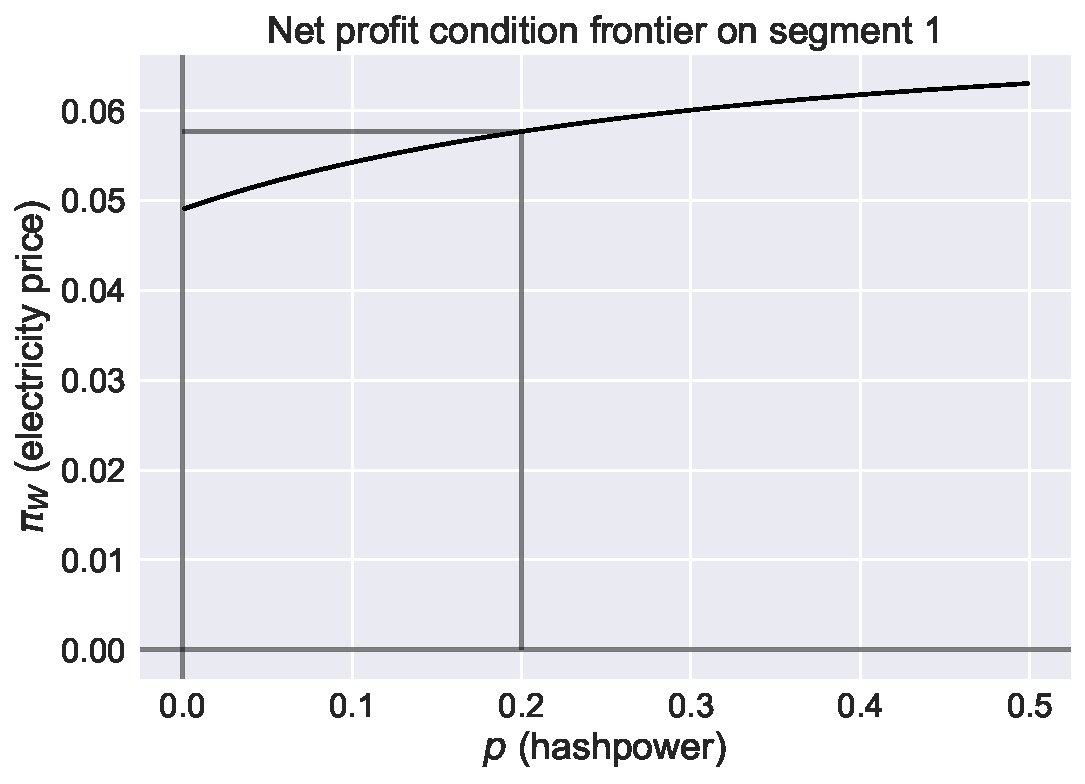
\includegraphics[width=0.45\textwidth]{../Figures/nbc_segment1_12a}
      \label{sub:nbc_segment1}
                         }
                         \hskip1em
    \subfloat[Net profit condition frontier on Segment 2.]{
      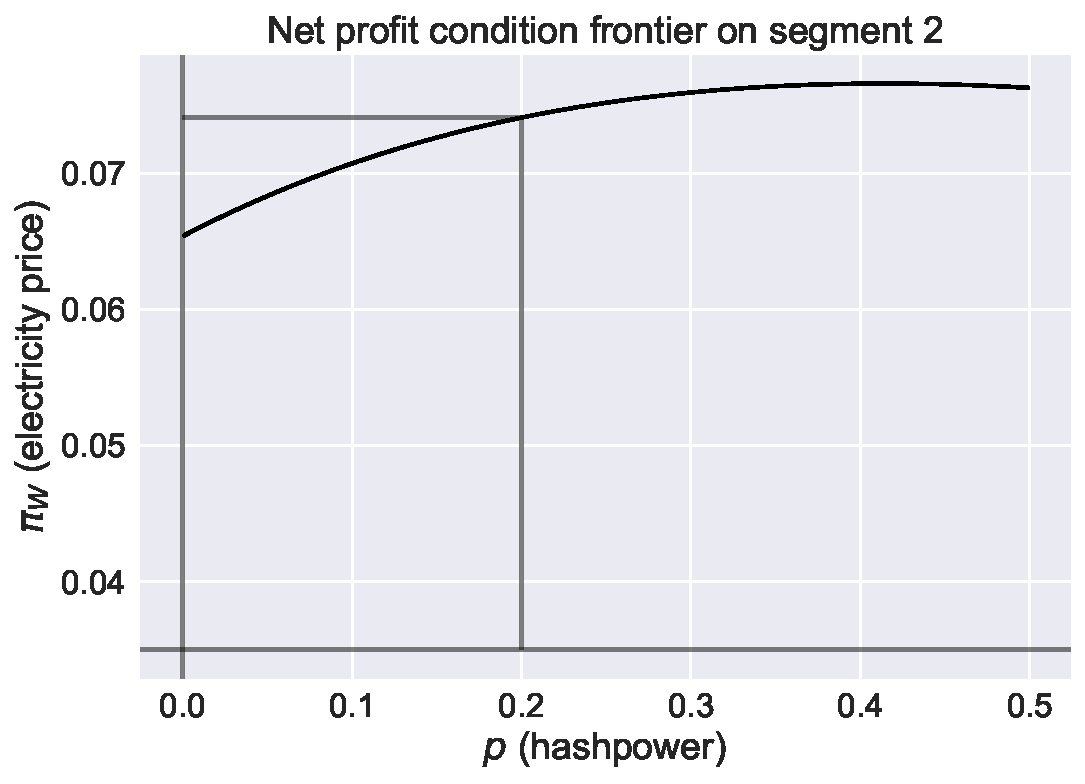
\includegraphics[width=0.45\textwidth]{../Figures/nbc_segment2_12b}
      \label{sub:nbc_segment2}
                         }
    \caption{Net profit condition frontier on Segment 1 and 2 for a selfish miner.}
    \label{fig:nbc_segments}
  \end{center}
\end{figure}
\noindent In absence of ruin considerations, selfish mining on Segment $1$ is profitable only if the price of electricity is lower than $0.058$, see \cref{sub:nbc_segment1}. Only when the selfish miner owns the totality of the hashpower, is selfish mining as profitable as following the protocol. On Segment $2$, the profitability is always greater than when following the protocol. The profitability on Segment $2$ holds in our case if the electricity price is lower than $0.074$, see \cref{sub:nbc_segment2}. It is interesting to note that by increasing the hashpower beyond a certain threshold we actually lower the profitability during Segment $2$. At higher hashpower levels, the probability of the Markov chain $(Z_n)_{n\geq 0}$ visiting state $0^\ast$ becomes small. In that case fewer blocks are being wasted, which in turn reduces the downward adjustment of the cryptopuzzle difficulty and hence the profitability during Segment 2.\\

\noindent Figure \ref{fig:rp_difficulty_adjusment} shows the ruin probability of a selfish miner and a miner following the protocol as a function of initial wealth for a range of electricity prices. 
\begin{figure}[!ht]
  \begin{center}
      % \subfloat[$\pi_W = 0.04$.]{
      % \includegraphics[width=0.45\textwidth]{Figures/rp_difficulty_adjusment_4}
      % \label{sub:rp_difficulty_adjusment_4}
      %                    }
                         \hskip1em
    \subfloat[$\pi_W = 0.05$.]{
      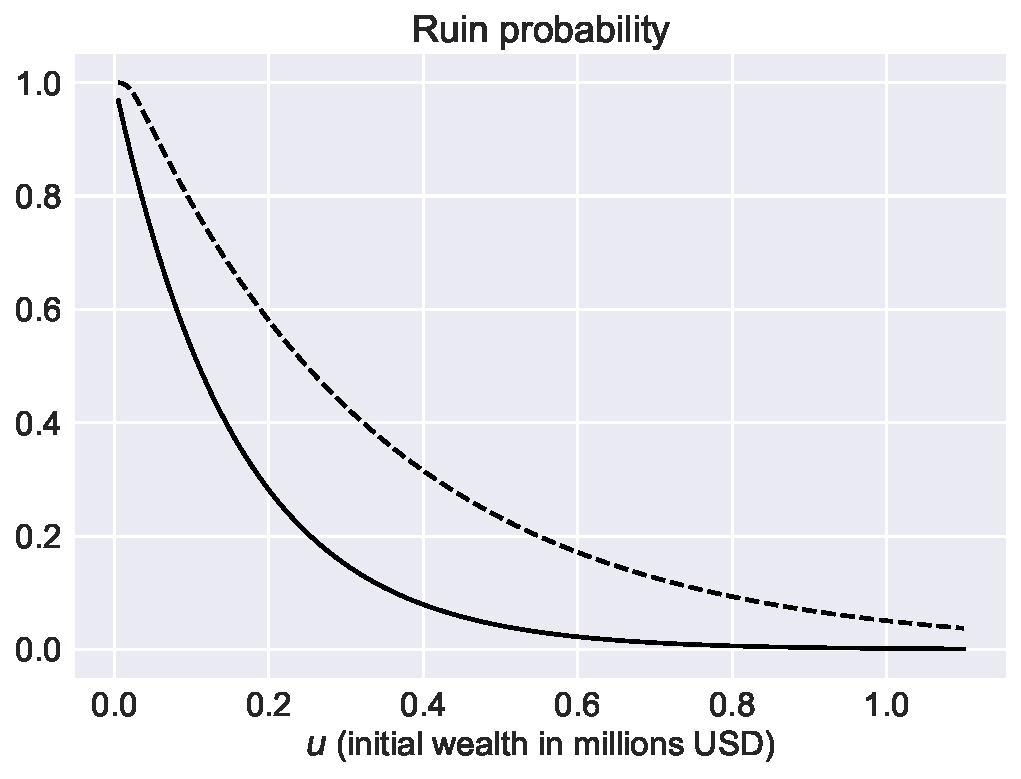
\includegraphics[width=0.45\textwidth]{../Figures/rp_difficulty_adjusment_5_13a}
      \label{sub:rp_difficulty_adjusment_5}
                         }
                         \hskip1em
       \subfloat[$\pi_W = 0.06$.]{
      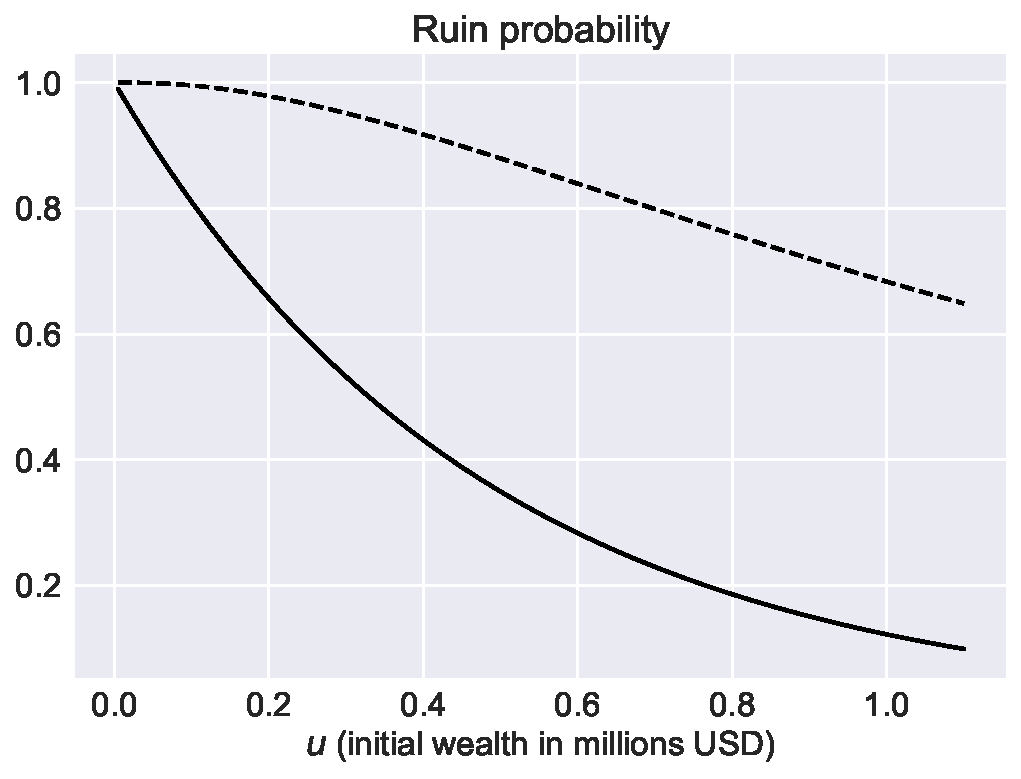
\includegraphics[width=0.45\textwidth]{../Figures/rp_difficulty_adjusment_6_13b}
      \label{sub:rp_difficulty_adjusment_6}
                         }
                         \hskip1em
    \subfloat[$\pi_W = 0.07$.]{
      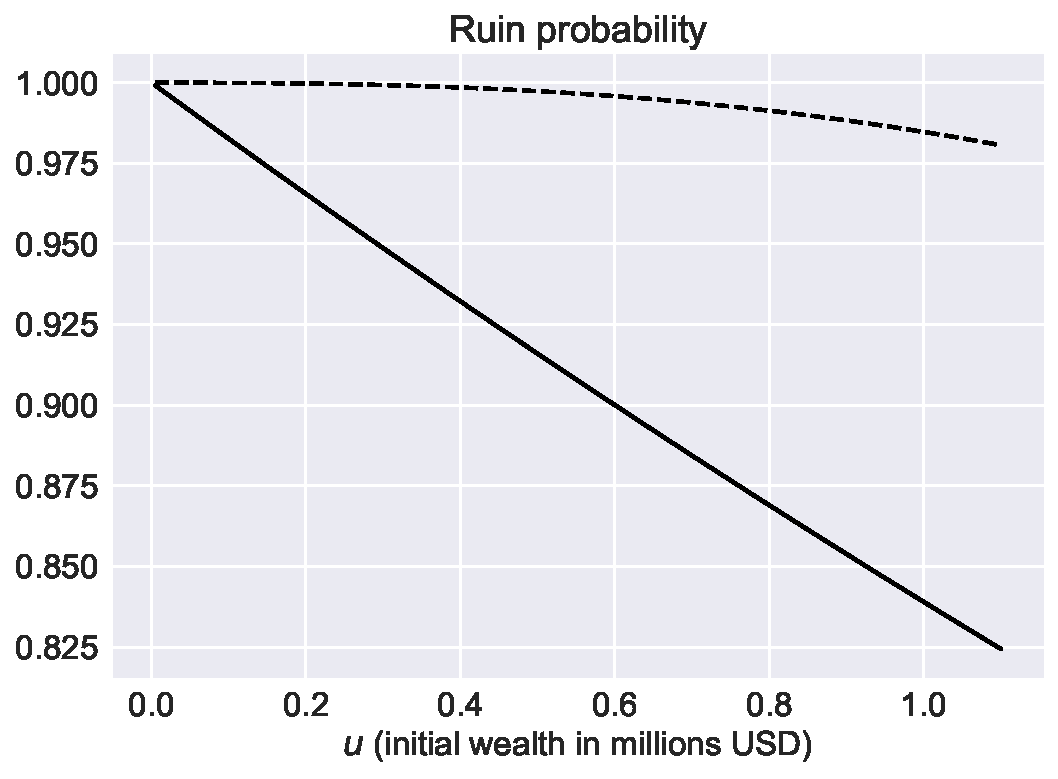
\includegraphics[width=0.45\textwidth]{../Figures/rp_difficulty_adjusment_7_13c}
      \label{sub:rp_difficulty_adjusment_7}
                         }
                         \hskip1em
       \subfloat[$\pi_W = 0.08$.]{
      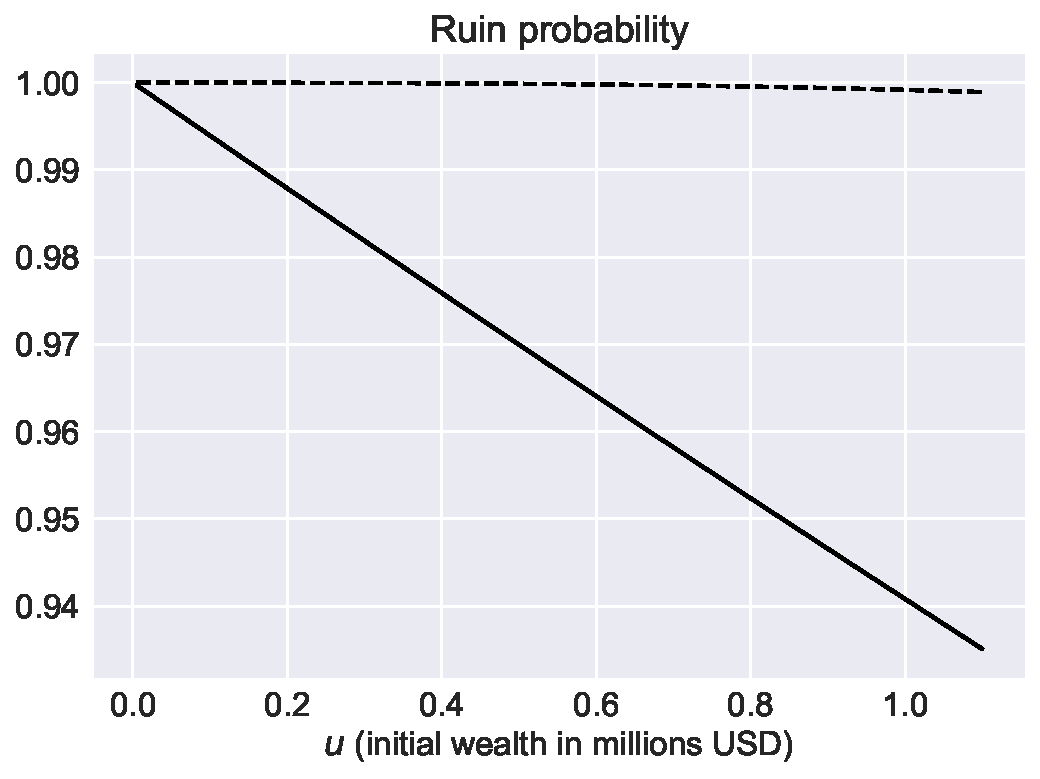
\includegraphics[width=0.45\textwidth]{../Figures/rp_difficulty_adjusment_8_13d}
      \label{sub:rp_difficulty_adjusment_8}
                         }
                         \hskip1em
    % \subfloat[$\pi_W = 0.09$.]{
    %   \includegraphics[width=0.45\textwidth]{../Figures/rp_difficulty_adjusment_9}
    %   \label{sub:rp_difficulty_adjusment_9}
    %                      }
    \caption{Ruin probability over two segments as a function of initial wealth of a miner following the protocol (solid) and a selfish miner (dashed) for various electricity prices with hashpower $p=0.2$ and connectivity $q=0.75$.}
    \label{fig:rp_difficulty_adjusment}
  \end{center}
\end{figure}
From a ruin probability perspective, reducing the difficulty adjustment does not compensate for the risk involved in implementing selfish mining. 

Figure \ref{fig:rev_difficulty_adjusment} displays the expected profit of a selfish miner and a miner following the protocol as a function of initial wealth for a range of electricity prices.
\begin{figure}[!ht]
  \begin{center}
      % \subfloat[$\pi_W = 0.04$.]{
      % \includegraphics[width=0.45\textwidth]{../Figures/rev_difficulty_adjusment_4}
      % \label{sub:rev_difficulty_adjusment_4}
      %                    }
                         \hskip1em
    \subfloat[$\pi_W = 0.05$.]{
      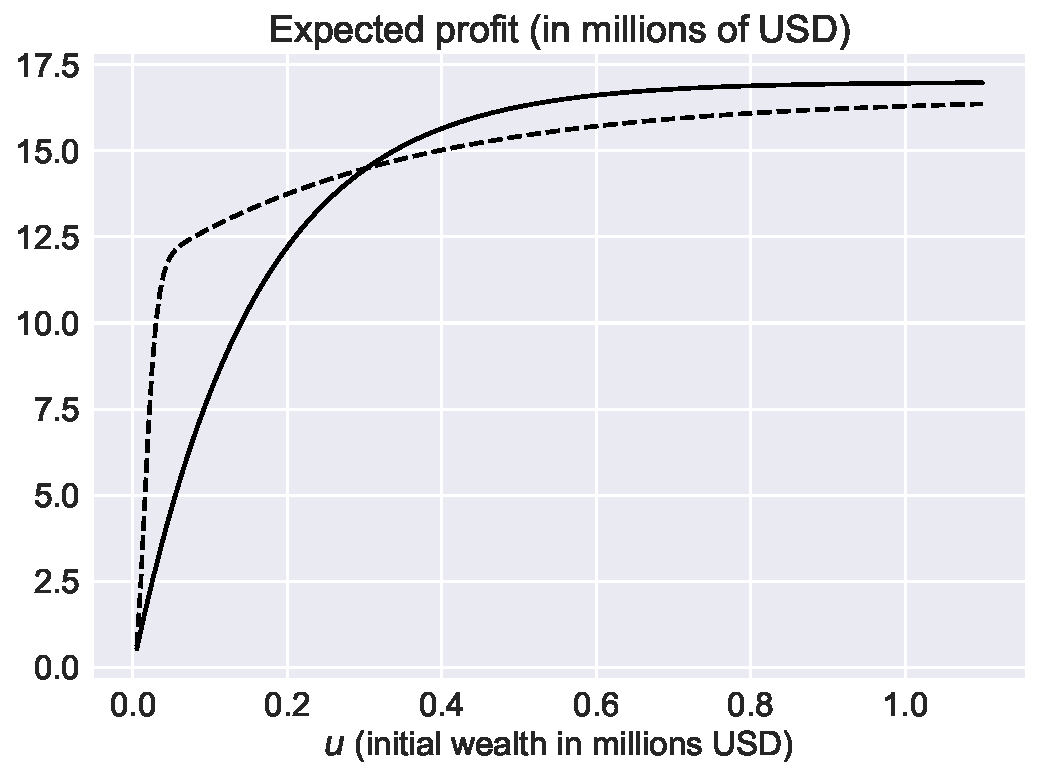
\includegraphics[width=0.45\textwidth]{../Figures/rev_difficulty_adjusment_5_14a}
      \label{sub:rev_difficulty_adjusment_5}
                         }
                         \hskip1em
       \subfloat[$\pi_W = 0.06$.]{
      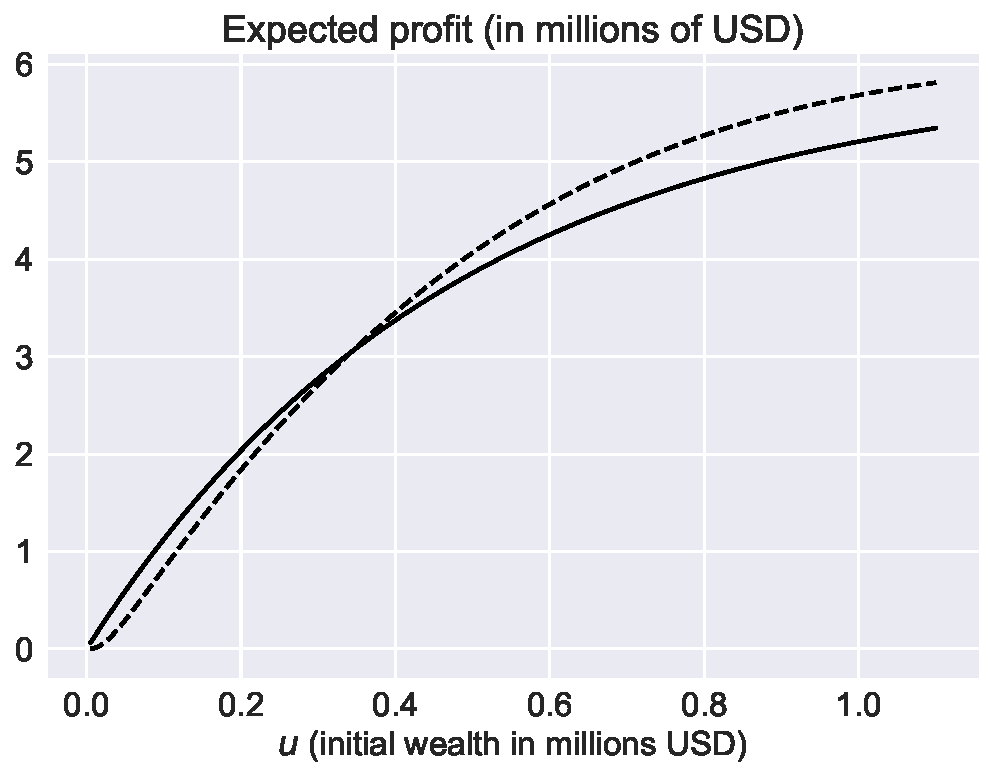
\includegraphics[width=0.45\textwidth]{../Figures/rev_difficulty_adjusment_6_14b}
      \label{sub:rev_difficulty_adjusment_6}
                         }
                         \hskip1em
    \subfloat[$\pi_W = 0.07$.]{
      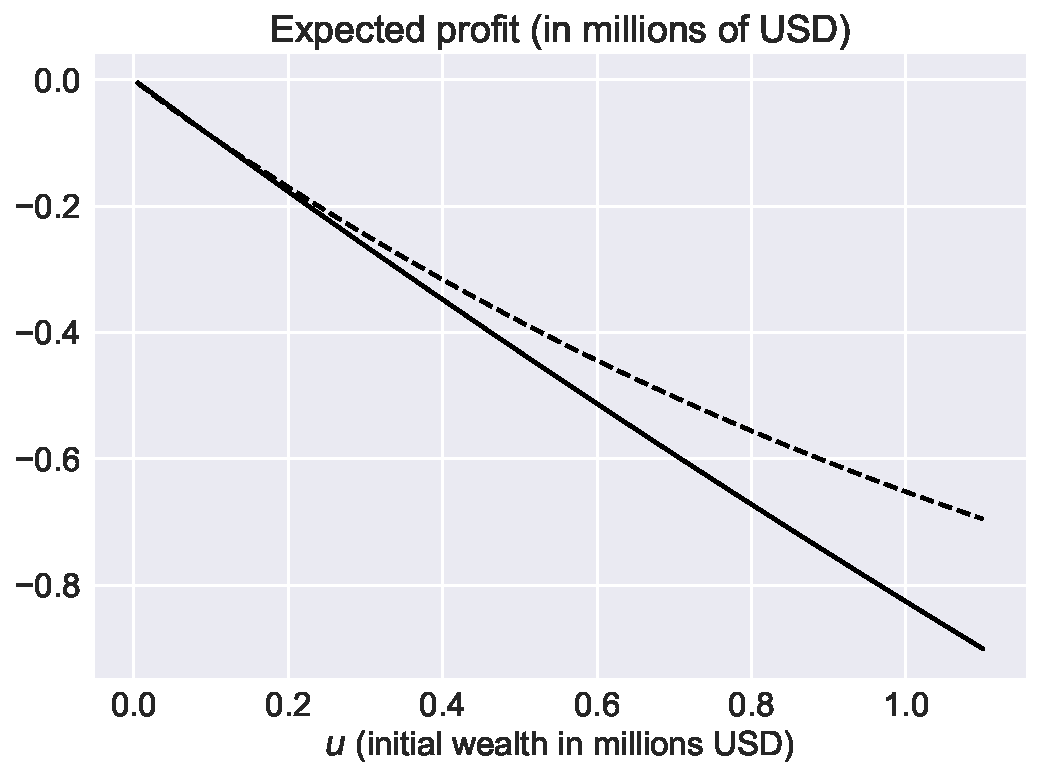
\includegraphics[width=0.45\textwidth]{../Figures/rev_difficulty_adjusment_7_14c}
      \label{sub:rev_difficulty_adjusment_7}
                         }
                         \hskip1em
       \subfloat[$\pi_W = 0.08$.]{
      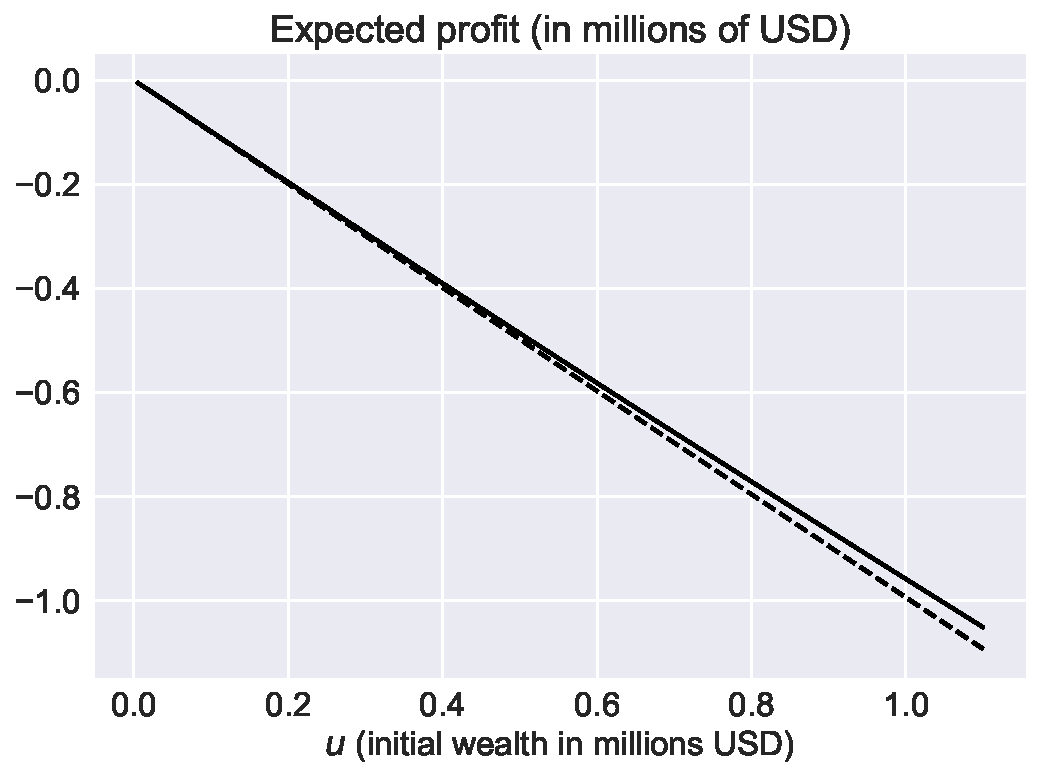
\includegraphics[width=0.45\textwidth]{../Figures/rev_difficulty_adjusment_8_14d}
      \label{sub:rev_difficulty_adjusment_8}
                         }
                         \hskip1em
    % \subfloat[$\pi_W = 0.09$.]{
    %   \includegraphics[width=0.45\textwidth]{../Figures/rev_difficulty_adjusment_9}
    %   \label{sub:rev_difficulty_adjusment_9}
    %                      }
    \caption{Expected profit over two segments as a function of initial wealth of a miner following the protocol (solid) and a selfish miner (dashed) for various electricity prices with hashpower $p=0.2$ and connectivity $q=0.75$.}
    \label{fig:rev_difficulty_adjusment}
  \end{center}
\end{figure}
 One can observe the different profit and loss profile of a selfish miner compared to that of a miner following the protocol on both segments. If the net profit condition holds when following the protocol, then it also holds for the second segment when blocks were withheld during the first segment. For electricity prices $\pi_W = 0.05, 0.06$, the expected profit as a function of $u$ reaches a plateau of level 
\begin{equation}\label{eq:plateau_protocol}
(c-b\lambda p)\times t
\end{equation}
when following the protocol, and 
\begin{equation}\label{eq:plateau_selfish}
(c-b\lambda_2 p)\times t_2,
\end{equation}
when selfish mining is applied during the first segment.  For $\pi_W = 0.05$, the plateau when following the protocol \eqref{eq:plateau_protocol} is higher than the plateau when withholding blocks \eqref{eq:plateau_selfish}, but the expected profit at lower initial wealth is greater for the selfish miner, see Figure \ref{sub:rev_difficulty_adjusment_5}. The exact opposite holds when $\pi_W = 0.06$, see Figure \ref{sub:rev_difficulty_adjusment_6}. The latter is probably the most desirable situation for a selfish miner. For $\pi_W = 0.07$, the net profit condition no longer holds when following the protocol which entails a loss, it holds however on the second segment of the selfish miner but it does not compensate for the loss incurred during the first segment, see Figure \ref{sub:rev_difficulty_adjusment_7}. Selfish mining helps at least in slightly mitigating the losses in this case. For electricity prices $\pi_W > 0.074$, the net profit condition breaks down in each case, resulting in huge losses for both the selfish and the honest miner (cf.\ Figure \ref{sub:rev_difficulty_adjusment_8} ).\\


\noindent The above analysis allowed us to distinguish situations where selfish mining can be considered worthwile and when it may not. In particular, it turns out that selfish mining can be advisable when following the protocol is not profitable. 

% \section{Nothing-at-stake in PoS}\label{sec:NaS}
% \newpage
% !TEX root = ../main_lecture_notes.tex
\chapter{Decentralization of blockchain system}\label{chap:decentralization}
Decentralization represents th efairness of the distribution of the accouunting right of the nodes in thee blockchain network. The consensus protocol must be designed so that the decision power does not eventually concentrate on a few nodes.\\

\noindent \cref{sec:decentralization_pos} focuses on the \PoS protocol by modelling the evolution of the stakes of the nodes by a stochastic process with reinforcement. \cref{sec:decentralization_pow} presents the concept of mining pool and discusses the threat they represent for the decentralized aspect of the network.

\section{Decentralization in PoS}\label{sec:decentralization_pos}
Rich get richer? Polya's urn
\subsection{Average stake own by each peer}
\subsection{Distribution of the stakes}
\section{Decentralization in PoW}\label{sec:decentralization_pow}
\subsection{Mining pools and reward systems}
\subsection{Mining pool risk analysis}

\newpage
% !TEX root = ../main_lecture_notes.tex
\chapter{Efficiency of blockchain systems}\label{chap:efficiency}

\section{A queueing model with bulk service}\label{sec:queue}
Blockchain users send transactions to the network of validators according to some rate $\lambda$. These transactions enter a queue of pending transactions. The validators select a subset of $b$ transactions to be recorded in the next block. The block is built by a leader elected via a consensus protocol. The block is then communicated to the other validators and the $b$ transactions exit the queue. We assume that building a block takes some exponentially distributed time with mean $\mu$. What we just described is exactly a single server with bulk service queueing system, described for instance in \citet{Bailey1954} and \citet{Chaudhry1981} with exponential arrival times, that processes $k$ items at a time, with an exponential service time. This a $M/M^b/1$ queue in Kendall's notation summarized in \cref{fig:blockchain_queue}.  
\begin{figure}[!ht]
\begin{center}
\begin{tikzpicture}[-, >=stealth', auto, semithick, node distance=1cm]

\tikzstyle{phantom block}=[rectangle, fill=white,draw=white, thick,text=black,scale=2]
\tikzstyle{block}=[rectangle, fill=white,draw=black,thick,text=black,scale=4]
\tikzstyle{Intensity}=[circle, fill=white,draw=blue,very thick, text=black,scale=1.2]
\tikzstyle{transaction pending}=[circle, fill=white,draw=blue,very thick, text=black,scale=1]
\tikzstyle{transaction considered}=[circle, fill=blue, text=black, scale=1]
\node[Intensity]    (1){$\lambda$};
\node[phantom block]  (2)[right of=1] {};
\node[transaction pending] (3)[right of=2] {};
\node[transaction pending] (4)[above of=3] {};
\node[transaction pending] (5)[above of=4] {};
\node[transaction pending] (6)[above of=5] {};
\node[transaction pending] (7)[below of=3] {};
\node[transaction pending] (8)[below of=7] {};
\path
(1) edge[->,bend left]     node{} (4)
    edge[->, bend right]     node{}          (7);

\node[Intensity]  (14)[above of=6]{$\mu$};
% \path
% (1) edge[->,bend left]     node{$\text{Exp}(\lambda)$}        (4)
%     edge[->, bend right]     node{}          (7);

\node[transaction considered] (3)[right of=2] {};
\node[transaction considered] (4)[above of=3] {};
\node[transaction considered] (5)[above of=4] {};
\node[transaction considered] (6)[above of=5] {};


\node[phantom block]  (10)[right of=3] {};
\node[block]  (11)[right of=10] {};
\path
(6) edge[->]   node{} (11)
(5) edge[->]   node{} (11)
(4) edge[->]   node{} (11)
(3) edge[->]   node{} (11)
;
\node[Intensity]  (12)[above of=11] {$\mu$};
\node[phantom block]  (13)[above of=12] {};

\path
(11) edge[-]     node{}        (12);
\path
(12) edge[->]     node{}        (13);

\end{tikzpicture}
\end{center}
\caption{Blockchain queue}
\label{fig:blockchain_queue}
\end{figure}
One specificity of this queue is that the server is always busy. Our goal is to assess the efficiency which is characterized by
\begin{itemize}
  \item Throughputs: Number of transaction being processed per time unit
  \item Latency: Average transaction confirmation time
\end{itemize} 
This can be done by studying the distribution of the number of pending transaction in the queue over the long run. A stationary state can only be reached if 
\begin{equation}\label{eq:stationarity_cond}
\mu \cdot b > \lambda.
\end{equation}
Denote by $N^q$ the length of the queue upon stationarity, The following result holds.
\begin{theo}
Assume that \eqref{eq:stationarity_cond} holds then $N^q$ is geometrically distributed 
$$
\mathbb{P}(N^q = n) = (1-p)\cdot p^n,\text{ } n\geq0
$$
where $p = 1/z^\ast$ and $z^\ast$ is the only root of 
$$
-\frac{\lambda}{\mu}z^{b+1}+z^b\left(\frac{\lambda}{\mu}+1\right) - 1,
$$
such that $|z^\ast$|>1.  
\end{theo}
\begin{proof}
Let $N^q_t$ be the number of transactions in the queue at time $t\geq0$ and $X_t$ the time elapsed since the last block was found. Further define
\[
P_{n}(x,t)\text{d}x  =\mathbb{P}[N_t^q = n, X_t \in(x, x + \text{dx})] 
\]
If $\lambda < \mu\cdot b$ holds then the process admits a limiting distribution given by 
\[
\underset{t\rightarrow\infty}{\lim}P_{n}(x,t) = P_{n}(x).
\]
Adding the variable $X_t$ is a known trick going back to \citet{Cox1955}, it allows us to make the process $(N_t^q)_{t\geq0}$ Markovian. We aim at finding the distribution of the queue length upon stationarity
\begin{equation}\label{eq:alpha_n}
\mathbb{P}(N^q=n):=\alpha_n =\int_{0}^\infty P_{n}(x)\text{d}x, \text{ }n\geq0.
\end{equation}
Consider the possible transitions over a small time lapse \text{h} during which no block is being generated. Over this time interval, either 
\begin{itemize}
  \item no transactions arrives
  \item one transaction arrives
\end{itemize}
We have for $n\geq1$
\[
P_{n}(x+h) = e^{-\mu h}\left[e^{-\lambda h}P_{n}(x)+\lambda h e^{-\lambda h}P_{n-1}(x)\right].
\]
Differentiating with respect to $h$ and letting $h\rightarrow0$ leads to 
\begin{equation}\label{eq:diff_eq_n_geq_1}
P_{n}'(x) = -(\lambda+\mu)P_{n}(x)+\lambda P_{n-1}(x),\text{ }n \geq1.
\end{equation}
Similarly for $n = 0$, we have 
\begin{equation}\label{eq:diff_eq_n_eq_0}
P_{0}'(x) = -(\lambda+\mu)P_{0}(x).
\end{equation}
We denote by 
$$
\xi(x)\text{d}x =\mathbb{P}(x\leq X< x+\text{d}x|X\geq x)= \mu\text{d}x,
$$
the hazard function of the block arrival time (constant as it is exponentially distributed). The system of differential equations \eqref{eq:diff_eq_n_geq_1}, \eqref{eq:diff_eq_n_eq_0} admits boundary conditions at $x = 0$ with 
\begin{equation}\label{eq:boundary_cond_1}
\begin{cases}
P_{n}(0) = \int_0^{+\infty} P_{n+b}(x)\xi(x)\text{d}x = \mu\alpha_{n+b},&n \geq1,\\
P_{0}(0) = \mu\sum_{n=0}^{b}\alpha_n,&n = 0,\ldots,b\\
\end{cases}
\end{equation}
Define the probability generating function of $N^q$ at some elapsed service time $x\geq 0$ as 
$$
G(z;x) = \sum_{n=0}^\infty P_{n}(x)z^n.
$$
By differentiating with respect to $x$, we get (using \eqref{eq:diff_eq_n_geq_1} and \eqref{eq:diff_eq_n_eq_0})
$$
\frac{\partial}{\partial x}G(z;x) = -\left[\lambda(1-z)+\mu\right]G(z;x),
$$
and therefore
$$
G(z;x) = G(z;0)\exp\left\{-\left[\lambda(1-z)+\mu\right]x\right\}.
$$
We get the probability generating function of $N^q$ by integrating over $x$ as 
\begin{equation}\label{eq:G_z_solve_ODE}
G(z) = \frac{G(z;0)}{\lambda(1-z)+\mu}.
\end{equation}
Using the boundary conditions \eqref{eq:boundary_cond_1}, we write 
\begin{eqnarray}
G(z;0) &= &\sum_{n = 0}^\infty P_{n}(0)z^n \nonumber\\
&= &P_{0}(0)+\sum_{n=1}^{+\infty}P_{n}(0)z^n\nonumber\\
&=& \mu\sum_{n = 0}^{b}\alpha_n  + \mu\sum_{n=1}^{+\infty}\alpha_{n+b} z^n\nonumber\\
&=& \mu\sum_{n = 0}^{b}\alpha_n + \mu z^{-b}\left[G(z)-\sum_{n = 0}^{b}\alpha_n z^n\right]\label{eq:G_z_0}
\end{eqnarray}
Replacing the left hand side of \eqref{eq:G_z_0} by \eqref{eq:G_z_solve_ODE}, multiplying on both side by $z^b$ and rearranging yields 
\begin{equation}\label{eq:G_z_as_rational_function}
\frac{G(z)}{M(z)}[z^b - M(z)] =\sum_{n=0}^{b-1}\alpha_n(z^b - z^n), 
\end{equation}
where $M(z) = \mu/(\lambda(1-z)+\mu)$. Using Rouche's theorem, we find that both side of the equation shares $b$ zeros inside the circle $\mathcal{C} = \{z\in\mathbb{C}\text{ ; }|z| <1+\epsilon\}$ for some epsilon. 
\begin{lemma}
Let $\mathcal{C}\in \mathbb{C}$ and $f$ and $g$ two holomorphic functions on $\mathcal{C}$. Let $\partial\mathcal{C}$ be the contour of $\partial\mathcal{C}$. If 
$$
|f(z)-g(z)|<|g(z)|\text{, }\forall z\in\partial\mathcal{C}
$$ 
then $Z_f-P_f = Z_g-P_g$, where $Z_f$, $P_f$, $Z_g$, and $P_g$ are the number of zeros and poles of $f$ and $g$ respectively.
\end{lemma}
We have $\partial\mathcal{C} =\{z\in\mathbb{C}\text{ ; }|z| =1+\epsilon\}$. The left hand side can be rewritten as
$$
G(z)\left[-\frac{\lambda}{\mu}z^{b+1} + \left(1 + \frac{\lambda}{\mu}\right)z^b -1\right].
$$
Define $f(z) = -\frac{\lambda}{\mu}z^{b+1} + \left(1 + \frac{\lambda}{\mu}\right)z^b -1$ and $g(z)=\left(1 + \frac{\lambda}{\mu}\right)z^b$. We have 
 $$
|f(z) - g(z)| = |-\frac{\lambda}{\mu}z^{b+1}-1|\leq \frac{\lambda}{\mu}(1+\epsilon)^{b+1}+1< \left(1 + \frac{\lambda}{\mu}\right)(1+\epsilon)^b= |g(z)| ,\text{ with }\epsilon \rightarrow 0. 
$$
Regarding the right hand side, define $f(z) = \sum_{n=0}^{b-1}\alpha_n(z^b - z^n)$ and $g(z) =\sum_{n=0}^{b-1}\alpha_nz^b $. We have 
$$
|f(z) - g(z)| < |\sum_{n=0}^{b-1}\alpha_n z^n| \leq \sum_{n=0}^{b-1}\alpha_n (1+\epsilon)^n<(1+\epsilon)^b\sum_{n=0}^{b-1}\alpha_n = |g(z)|.
$$
We deduce from Rouche's theorem that both sides have $b$ share roots inside $\mathcal{C}$. Note that one of them is $1$, and we denote by $z_k$, $k = 1,\ldots, b-1$ the remaining $b-1$ roots. Given the polynomial form of the right hand side of \eqref{eq:G_z_as_rational_function}, the fundamental theorem of algebra indicates that the number of zero is $b$. Given the left hand side 
$$
G(z)\left[-\frac{\lambda}{\mu}z^{b+1} + \left(1 + \frac{\lambda}{\mu}\right)z^b -1\right].
$$
we deduce that there is one zeros outside $\mathcal{C}$, we can further show that it is a real number $z^\ast$. Multiplying both side of \eqref{eq:G_z_as_rational_function} by $(z-1)\prod_{k =1}^{b-1}(z-z_k)$, and using $G(1)=1$ yields
$$
G(z) = \frac{1-z^\ast}{z-z^{\ast}}.
$$
$N^q$ is then a geometric random variable with parameter $p = \frac{1}{z^\ast}.$
\end{proof}
\section{Latency and throughputs computation}\label{sec:latency_throughputs}
\newpage

\bibliography{../blockastics}
\bibliographystyle{plainnat}

\end{document}


